%%%%%%%%%%%%%%%%%%%%%%%%%%%%%%%%%%%%%%%%%%%%%%%%%%%%%%%%%%%%%%%%%%%%%%%%%%%%%%%%
%% Plantilla de memoria en LaTeX para la EIF - Universidad Rey Juan Carlos
%%
%% Por Gregorio Robles <grex arroba gsyc.urjc.es>
%%     Grupo de Sistemas y Comunicaciones
%%     Escuela de Ingeniería de Fuenlabrada
%%     Universidad Rey Juan Carlos
%% (muchas ideas tomadas de Internet, colegas del GSyC, antiguos alumnos...
%%  etc. Muchas gracias a todos)
%%
%% La última versión de esta plantilla está siempre disponible en:
%%     https://github.com/gregoriorobles/plantilla-memoria
%%
%% Para obtener PDF, ejecuta en la shell:
%%   make
%% (las imágenes deben ir en PNG o JPG)

%%%%%%%%%%%%%%%%%%%%%%%%%%%%%%%%%%%%%%%%%%%%%%%%%%%%%%%%%%%%%%%%%%%%%%%%%%%%%%%%

\documentclass[a4paper, 11pt]{book}
%\usepackage[T1]{fontenc}

\usepackage[a4paper, left=2.5cm, right=2.5cm, top=3cm, bottom=3cm]{geometry}
\usepackage{times}
\usepackage[utf8]{inputenc}
\usepackage[spanish]{babel} % Comenta esta línea si tu memoria es en inglés
\usepackage{url}
%\usepackage[dvipdfm]{graphicx}
\usepackage{graphicx}
\usepackage{float}  %% H para posicionar figuras
\usepackage[nottoc, notlot, notlof, notindex]{tocbibind} %% Opciones de índice
\usepackage{latexsym}  %% Logo LaTeX
\usepackage{glossaries}
\glsenablehyper
\usepackage{hyperref}
\usepackage{tikz}% crear árboles
\usepackage{minted}% código resaltado.
\usemintedstyle{colorful}
\setcounter{tocdepth}{4}%Profundidad de la tabla de contenidos
% Ajustar los valores de los contadores
\setcounter{secnumdepth}{4}

% Configuración de hyperref para resaltar los enlaces
\hypersetup{
    colorlinks=true,       % false: boxed links; true: colored links
    linkcolor=blue,          % color of internal links (change box color with linkbordercolor)
    citecolor=blue,        % color of links to bibliography
    filecolor=blue,         % color of file links
    urlcolor=blue        % color of external links
}
\makeglossaries

\title{Memoria del Proyecto}
\author{Víctor Jesús Temprano Hernández}

\renewcommand{\baselinestretch}{1.5}  %% Interlineado

\begin{document}

\renewcommand{\refname}{Bibliografía}  %% Renombrando
\renewcommand{\appendixname}{Apéndice}


%%%%%%%%%%%%%%%%%%%%%%%%%%%%%%%%%%%%%%%%%%%%%%%%%%%%%%%%%%%%%%%%%%%%%%%%%%%%%%%%
% PORTADA

\begin{titlepage}
\begin{center}

\includegraphics[scale=0.6]{img/URJ_logo_Color_POS.png}

\vspace{1.75cm}

\LARGE
ESCUELA DE INGENIERÍA DE FUENLABRADA
\vspace{1cm}

\LARGE
GRADO EN INGENIERÍA EN TELEMÁTICA

\vspace{1cm}
\LARGE
\textbf{TRABAJO FIN DE GRADO}

\vspace{2cm}

\Large
VISUALIZACIÓN EN REALIDAD VIRTUAL DE DATOS AERONÁUTICOS
CON CONTEXTO GEOESPACIAL

\vspace{2cm}

\large
Autor : Víctor Jesús Temprano Hernández \\
Tutor : Dr. Jesús M. González Barahona\\
\vspace{1cm}

\large
Curso académico 2022/2023

\end{center}
\end{titlepage}

\newpage
\mbox{}
\thispagestyle{empty} % para que no se numere esta pagina



%%%%%%%%%%%%%%%%%%%%%%%%%%%%%%%%%%%%%%%%%%%%%%%%%%%%%%%%%%%%%%%%%%%%%%%%%%%%%%%%
%%%% Para firmar
%\clearpage
%\pagenumbering{gobble}
%\chapter*{}
%
%\vspace{-4cm}
%\begin{center}
%\LARGE
%\textbf{Trabajo Fin de Grado/Máster}
%
%\vspace{1cm}
%\large
%Visualización en Realidad Virtual de Datos Aeronáuticos
%con Contexto Geoespacial\\
%\vspace{1cm}
%\large
%\textbf{Autor :} Víctor Jesús Temprano Hernández \\
%\textbf{Tutor :} Dr. Jesús M. González Barahona
%
%\end{center}
%
%\vspace{1cm}
%La defensa del presente Proyecto Fin de Carrera se realizó el día \qquad$\;\,$ de \qquad\qquad\qquad\qquad \newline de 2023, siendo calificada por el siguiente tribunal:
%
%
%\vspace{0.5cm}
%\textbf{Presidente:}
%
%\vspace{1.2cm}
%\textbf{Secretario:}
%
%\vspace{1.2cm}
%\textbf{Vocal:}
%
%
%\vspace{1.2cm}
%y habiendo obtenido la siguiente calificación:
%
%\vspace{1cm}
%\textbf{Calificación:}
%
%
%\vspace{1cm}
%\begin{flushright}
%Fuenlabrada, a \qquad$\;\,$ de \qquad\qquad\qquad\qquad de 2023
%\end{flushright}
%

%%%%%%%%%%%%%%%%%%%%%%LICENCIA%%%%%%%%%%%%%%%%%%%%%%%%%%%%
\vfill
\begin{flushright}
\begin{minipage}{0.65\textwidth}
{\footnotesize 
\noindent©2023 Víctor Jesús Temprano Hernández\\ 
Algunos derechos reservados\\
Este documento se distribuye bajo la licencia\\
“Atribución-CompartirIgual 4.0 Internacional” de Creative Commons,\\
disponible en  \\
\url{https://creativecommons.org/licenses/by-sa/4.0/deed.es}
}

\end{minipage}
\end{flushright}
%%%%%%%%%%%%%%%%%%%%%%%%%%%%%%%%%%%%%%%%%%%%%%%%%%%%%%%%%%%

%%%%%%%%%%%%%%%%%%%%%%%%%%%%%%%%%%%%%%%%%%%%%%%%%%%%%%%%%%%%%%%%%%%%%%%%%%%%%%%%
%%%% Dedicatoria

\chapter*{Dedicatoria}
En honor a mi padre, aunque no estés entre nosotros, siempre estarás presente en cada logro que alcanzo. Se que te sentirás orgulloso de mí, siempre te llevaré presente en mi corazón. Tu memoria y tu legado vivirá eternamente en mí.

%%%%%%%%%%%%%%%%%%%%%%%%%%%%%%%%%%%%%%%%%%%%%%%%%%%%%%%%%%%%%%%%%%%%%%%%%%%%%%%%
%%%% Agradecimientos

\chapter*{Agradecimientos}
%\addcontentsline{toc}{chapter}{Agradecimientos} % si queremos que aparezca en el índice
\markboth{AGRADECIMIENTOS}{AGRADECIMIENTOS} % encabezado 

En primer lugar quiero expresar mi profundo agradecimiento a mi mujer por acompañarme en cada uno de mis desafíos, y especialmente en este, donde ha asumido el papel de padre y madre para permitirme enfrentar este reto. Este trabajo no habría sido posible sin tu apoyo incondicional.\\
También quiero dar las gracias a mi madre por recordarme que la vida es impredecible y que siempre es mejor tarde que nunca.\\
Y por último a mi tutor Jesús María González Barahona, por adaptarse a mis horarios caóticos y comprender mis necesidades. Su flexibilidad ha sido fundamental en el desarrollo de este proyecto.

%%%%%%%%%%%%%%%%%%%%%%%%%%%%%%%%%%%%%%%%%%%%%%%%%%%%%%%%%%%%%%%%%%%%%%%%%%%%%%%%
%%%% Resumen

\chapter*{Resumen}
\markboth{RESUMEN}{RESUMEN} % encabezado
Voy a desarrollar un conjunto de herramientas que simplifiquen la creación de escenarios \gls{3D} para la representación y visualización de datos relacionados con la aviación. Estas herramientas permitirán crear aplicaciones que muestren información en tiempo real o datos almacenados en el dispositivo para una visualización sin conexión.

Además, estas herramientas proporcionarán al usuario una experiencia inmersiva mediante el uso de tecnologías de realidad virtual. Esto permitirá al usuario sumergirse en el escenario y comprender de manera intuitiva el estado del espacio aéreo. Los usuarios podrán desplazarse a través del escenario sobre el terreno utilizando dispositivos de realidad virtual y explorar los datos de manera interactiva. Todo esto se logrará mediante una interfaz de usuario que integre un conjunto de componentes diseñados para la visualización de la información. Estos componentes formarán parte del escenario como elementos adicionales, ofreciendo una visualización completa de los datos en un entorno contextualizado.

Crearé un prototipo final que mostrará el conjunto de herramientas y componentes desarrollados. Este prototipo proporcionará un escenario cercano a un aeropuerto, donde el usuario podrá sumergirse en la escena y consultar datos de aviación en tiempo real. Además, el prototipo incluirá la representación de edificios y un terreno con alturas definidas, que se visualizará utilizando la textura de un mapa satelital de la zona seleccionada. Esto permitirá brindar mayor realismo a la escena y una experiencia inmersiva al usuario.

%%%%%%%%%%%%%%%%%%%%%%%%%%%%%%%%%%%%%%%%%%%%%%%%%%%%%%%%%%%%%%%%%%%%%%%%%%%%%%%%
%%%% Resumen en inglés

\chapter*{Summary}
%\addcontentsline{toc}{chapter}{Summary} % si queremos que aparezca en el índice
\markboth{SUMMARY}{SUMMARY} % encabezado

I will develop a set of tools that simplify the creation of \gls{3D} scenarios for the representation and visualization of aviation related data. These tools will enable the creation of applications that display real time information or cache data on the device for offline visualization.

Furthermore, these tools will provide the user with an immersive experience through the use of virtual reality technologies. This will allow the user to immerse themselves in the scenario and intuitively understand the state of the airspace. Users will be able to navigate through the scenario and explore the data interactively using virtual reality devices. All of this will be achieved through a user interface that integrates a set of components designed for information visualization. These components will be integrated into the scenario as additional elements, offering a comprehensive visualization of the data in a contextualized environment.

I will create a final prototype that showcases the developed set of tools and components. This prototype will provide a scenario resembling an airport, where users can immerse themselves in the scene and access real time aviation data. Additionally, the prototype will include the representation of buildings and a terrain with defined heights, which will be visualized using the texture of a satellite map of the selected area. This will enhance the realism of the scene and provide an immersive experience for the user.

%%%%%%%%%%%%%%%%%%%%%%%%%%%%%%%%%%%%%%%%%%%%%%%%%%%%%%%%%%%%%%%%%%%%%%%%%%%%%%%%
%%%%%%%%%%%%%%%%%%%%%%%%%%%%%%%%%%%%%%%%%%%%%%%%%%%%%%%%%%%%%%%%%%%%%%%%%%%%%%%%
% ÍNDICES %
%%%%%%%%%%%%%%%%%%%%%%%%%%%%%%%%%%%%%%%%%%%%%%%%%%%%%%%%%%%%%%%%%%%%%%%%%%%%%%%%

% Las buenas noticias es que los índices se generan automáticamente.
% Lo único que tienes que hacer es elegir cuáles quieren que se generen,
% y comentar/descomentar esa instrucción de LaTeX.

%%%% Índice de contenidos
\tableofcontents 
%%%% Índice de figuras
\cleardoublepage
%\addcontentsline{toc}{chapter}{Lista de figuras} % para que aparezca en el indice de contenidos
\listoffigures % indice de figuras
%%%% Índice de tablas
%\cleardoublepage
%\addcontentsline{toc}{chapter}{Lista de tablas} % para que aparezca en el indice de contenidos
%\listoftables % indice de tablas


%%%%%%%%%%%%%%%%%%%%%%%%%%%%%%%%%%%%%%%%%%%%%%%%%%%%%%%%%%%%%%%%%%%%%%%%%%%%%%%%
%%%%%%%%%%%%%%%%%%%%%%%%%%%%%%%%%%%%%%%%%%%%%%%%%%%%%%%%%%%%%%%%%%%%%%%%%%%%%%%%
% INTRODUCCIÓN %
%%%%%%%%%%%%%%%%%%%%%%%%%%%%%%%%%%%%%%%%%%%%%%%%%%%%%%%%%%%%%%%%%%%%%%%%%%%%%%%%

\cleardoublepage
\chapter{Introducción}
\label{sec:intro} % etiqueta para poder referenciar luego en el texto con ~\ref{sec:intro}
\pagenumbering{arabic} % para empezar la numeración de página con números
El proyecto se enfoca en la creación de un conjunto de herramientas que proporcionen una plataforma para la visualización de datos aéreos en un entorno tridimensional, brindando al usuario una experiencia inmersiva.

Gracias al avance significativo de los dispositivos de realidad virtual y la disponibilidad de librerías de desarrollo que facilitan la creación de aplicaciones \gls{3D}, se creará una plataforma que ofrezca funcionalidades de visualización de datos aéreos en un entorno geoespacial \textsc{3D}. Este entorno estará rodeado de entidades que crean un contexto que proporciona una experiencia más realista para el usuario.

Estas herramientas estarán dirigidas a un entorno web, con el objetivo de ser compatibles tanto en dispositivos móviles como en entornos de escritorio o en dispositivos de realidad virtual.

Los datos con los que voy a trabajar, procederán de servicios web gratuitos y podrán ser obtenidos en tiempo real o desde una caché local. Estos datos nos proporcionaran información sobre los vuelos y también información sobre las alturas del terreno y edificios presentes en la escena tridimensional.

Para lograr este propósito, construiré todo el prototipo utilizando el \Gls{framework} de desarrollo llamado \textsc{A-Frame}\footnote{\url{https://aframe.io/}}. Este \emph{framework} proporciona una capa de abstracción fácil de usar y comprender, lo cual facilita una implementación más sencilla de conceptos más complejos como la creación de escenas en realidad virtual y la manipulación e interacción de objetos \textsc{3D}. 
Estos aspectos se analizarán con mayor detalle en secciones posteriores.

La razón principal de usar la tecnología \textsc{A-Frame} es centrar nuestro esfuerzo en la codificación del modelo negocio acelerando el proceso de desarrollo de la gestión y generación de modelos \textsc{3D}, que es un proceso complejo y laborioso.

Es importante destacar que la tecnología \textsc{A-Frame} se basa en \textsc{HTML5} para crear un ecosistema de componentes y geometrías utilizando elementos \textsc{HTML}. Esta tecnología permite aprovechar la potencia y flexibilidad de la librería \textsc{Three.js} a través de un lenguaje de marcado simplificado, acelerando así el desarrollo de aplicaciones \textsc{3D}. \textsc{A-Frame} facilita la creación de escenarios tridimensionales al proporcionar una forma más intuitiva y rápida de trabajar con \textsc{Three.js}.

A su vez, \textsc{Three.js} se construye sobre \textsc{\gls{WebGL}}\footnote{\url{https://www.khronos.org/webgl/}}, una \Gls{API} de gráficos en \textsc{3D} basada en \textsc{OpenGL}. Esto permite a los desarrolladores web acceder directamente a la capacidad de procesamiento de gráficos de la tarjeta gráfica del dispositivo mediante el uso de \emph{JavaScript} para controlar la \gls{renderización} y la manipulación de los objetos \textsc{3D}.

Esta arquitectura nos ofrece la ventaja de poder trabajar en un nivel de abstracción inferior cuando necesitamos abordar tareas más complejas relacionadas con objetos \textsc{3D}. Además, podemos crear componentes reutilizables que serán útiles tanto en el proyecto actual como en proyectos futuros basados en la tecnología \textsc{A-Frame}.

En resumen, la combinación de \textsc{HTML5}, \textsc{A-Frame}, \textsc{Three.js} y \textsc{WebGL} nos brinda un conjunto de herramientas poderosas para el desarrollo de experiencias \textsc{3D} en entornos web, permitiéndonos aprovechar al máximo el potencial de la tarjeta gráfica del dispositivo y facilitando la reutilización de componentes en futuros proyectos.

A continuación en la figura ~\ref{figura:mapaTecnologias}, muestro un mapa donde se puede visualizar como se relacionan las tecnologías y los servicios de datos principales en las que se basará el prototipo que voy a realizar. 
 \begin{figure}[h]
    \centering
    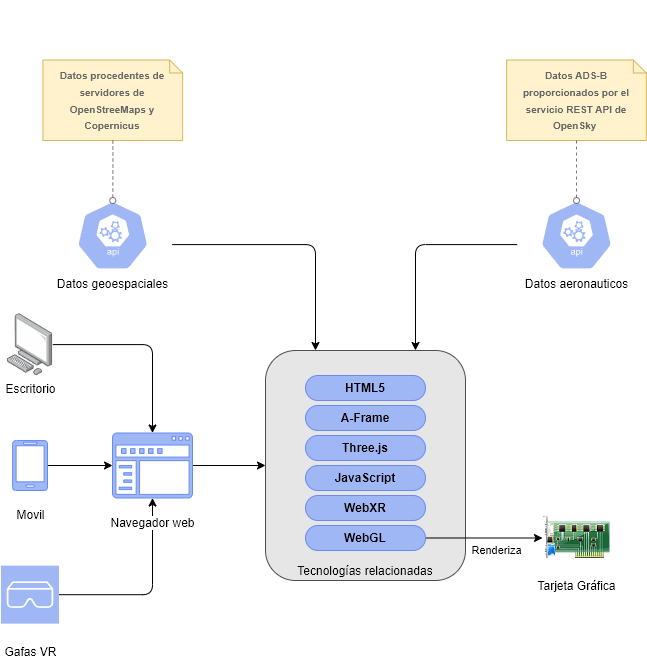
\includegraphics[bb=0 0 564 586, width=13cm, keepaspectratio]{img/mapaFuncional.drawio.png}
    \caption{Mapa de tecnologías}
    \label{figura:mapaTecnologias}
 \end{figure}
\clearpage
\section{Motivación}
\label{sec:motivación}

Después de trabajar durante seis años en el proyecto \emph{fullstack} \textsc{\gls{gis}} llamado \textsc{IGEA} de la compañía \textsc{Indra}, tuve la oportunidad de asumir la responsabilidad de integrar el núcleo del proyecto software \textsc{IGEA}\footnote{\url{https://www.indracompany.com/sites/default/files/indra_in_grid_esp_baja.pdf}} en una nueva aplicación de software para el proyecto \textsc{iTEC}, el cual se enfoca en la visualización y gestión de espacios aéreos europeos. Este desafío representó un hito muy interesante en mi carrera, ya que me permitió salir de mi zona de confort y experimentar un crecimiento de conocimientos sobre entornos de programación en 3D sobre la tecnología \textsc{JAVA}.

El objetivo principal de esta integración fue reutilizar los componentes centrales de \textsc{IGEA} para desarrollar una interfaz gráfica que facilitara a los usuarios administrativos la visualización y manipulación de datos aéreos de manera más intuitiva. Además, se aprovecharon las herramientas gráficas desarrolladas a lo largo de los más de veinte años de experiencia del proyecto \textsc{IGEA} para gestionar de manera efectiva los datos. Este enfoque permitió crear una solución poderosa y eficiente en poco tiempo para el proyecto \textsc{iTEC}.

Desde el momento en que comencé a buscar un proyecto para la finalización de mis estudios y comencé a analizar las posibilidades que me proporcionaba un proyecto basado en una aplicación \textsc{3D}, me di cuenta de la interesante oportunidad de combinar mi experiencia laboral previa con las demandas de este proyecto. 
Explorando las posibilidades se me ocurrió la idea de visualizar información aeroespacial en un entorno de realidad virtual, ya que la representación bidimensional de datos aéreos que proporcionan la mayoría de las aplicaciones web actuales resulta limitada y la dimensión de altura es fundamental para la gestión de espacios aereos. Además, la posibilidad de formar parte activa de la escena añade un valor significativo a las aplicaciones de consultas de datos. En este sentido, el futuro de estas aplicaciones parece prometedor.

\section{Contexto}
\label{sec:contexto}
Durante la última década, la recopilación y transmisión de datos en tiempo real se han vuelto más accesibles gracias a la fusión de las tecnologías web junto a las tecnologías de vigilancia aérea, lo que ha creado nuevas oportunidades para el desarrollo de aplicaciones y servicios web que permiten a los usuarios visualizar el tráfico aéreo y los datos de vuelo en tiempo real.

Uno de los sistemas que ha experimentado un gran desarrollo y éxito en el ámbito aeronáutico es el sistema de vigilancia automática dependiente de difusión \textsc{ADS-B}~\ref{sec:adsb}. Este sistema permite que las aeronaves transmitan información precisa de sus sensores, como la posición, velocidad, altitud, orientación, entre otros datos relevantes. 
El crecimiento de esta tecnología ha llevado a empresas y plataformas como FlightRadar24 y OpenSky a expandir sus redes y ofrecer servicios, incluso gratuitos, que proporcionan estos metadatos a través de la web. Esto ha impulsado el aumento de aplicaciones que muestran información de vuelos en tiempo real mediante mapas interactivos.

FlightRadar24, una empresa destacada en este campo, ofrece servicios web que muestran información en tiempo real sobre vuelos en un mapa bidimensional. Además del seguimiento de vuelos, proporciona detalles como el origen y destino de los vuelos, números de vuelo, tipos de aviones, altitudes, rumbos y velocidades.

OpenSky\ref{sec:opensky}, por su parte, es otra plataforma relevante que recopila y proporciona datos de vuelo en tiempo real. Además de mostrar información sobre los vuelos, OpenSky ha contribuido significativamente a la investigación en el ámbito de la aviación al proporcionar acceso a su base de datos para investigadores y desarrolladores interesados en analizar y utilizar datos aeroespaciales.

El avance en la recopilación y transmisión de datos en tiempo real, junto con el crecimiento de los sistemas \textsc{ADS-B}, ha sentado las bases para el desarrollo de aplicaciones y servicios web que permiten la visualización de información aeronáutica en tiempo real en dos dimensiones.

Sin embargo, el panorama se ha ampliado aún más con el aumento en los últimos años de servicios de sistemas de información geográfica para datos espaciales, como el programa \textsc{Copernicus} y los servicios ofrecidos por \textsc{Google} a través de su \textsc{API} \textsc{Google Earth Engine}. Estos servicios nos brindan acceso a una amplia variedad de mapas y datos geoespaciales que podemos utilizar para crear escenas más realistas y contextualizadas.

Al aprovechar los datos proporcionados por estos servicios, podemos mejorar la visualización de información aeronáutica al agregar capas adicionales, como imágenes satelitales y datos de relieve. Esto nos permite crear escenarios más ricos y detallados que ofrecen una representación más precisa y completa de la información aeronáutica en tiempo real.

La migración de funcionalidades de las aplicaciones actuales en dos dimensiones hacia aplicaciones \textsc{3D} inmersivas en realidad virtual tiene el potencial de llevar la experiencia de visualización de datos aeroespaciales a un nivel superior. Al hacerlo, se puede lograr una representación más completa y envolvente de los datos aeroespaciales.

Imaginar la inclusión de un controlador de espacios aéreos dentro de un entorno tridimensional, proporcionando la capacidad de gestionar aviones en tiempo real, es sumamente emocionante. Con un desarrollo adecuado, esta idea tiene el potencial de revolucionar la forma en que se controlan y gestionan los espacios aéreos.

La idea de poder estar en un aeropuerto, esperando a un familiar y tener la posibilidad de seguir el aterrizaje y visualizar lo que están viendo desde el avión a través de una experiencia en realidad virtual también resulta emocionante. Esta perspectiva nos permitiría tener una conexión más inmersiva con la experiencia de vuelo y compartir virtualmente el viaje con nuestros seres queridos. 

%%%%%%%%%%%%%%%%%%%%%%%%%%%%%%%%%%%%%%%%%%%%%%%%%%%%%%%%%%%%%%%%%%%%%%%%%%%%%%%%
%%%%%%%%%%%%%%%%%%%%%%%%%%%%%%%%%%%%%%%%%%%%%%%%%%%%%%%%%%%%%%%%%%%%%%%%%%%%%%%%
% OBJETIVOS %
%%%%%%%%%%%%%%%%%%%%%%%%%%%%%%%%%%%%%%%%%%%%%%%%%%%%%%%%%%%%%%%%%%%%%%%%%%%%%%%%

\newpage
\section{Objetivo general}
\label{sec:objetivoGeneral}
El objetivo general del proyecto consiste en investigar y adquirir conocimientos sobre tecnologías de realidad virtual y el framework \textsc{A-Frame}, el cual permite la creación de aplicaciones \gls{3D} para visualizar datos. Estas aplicaciones pueden ser ejecutadas en un navegador y ser utilizadas tanto en entornos de escritorio como en dispositivos móviles y dispositivos de realidad virtual, como los \textsc{Oculus Quest}.

En este contexto, se desarrollará un prototipo que constará de un conjunto de herramientas altamente configurable que siente las bases para facilitar la creación de escenas \textsc{3D}. 
Estas escenas permitirán la visualización de datos aeronáuticos, como vuelos en movimiento, en un contexto geoespacial. Además, se podrán visualizar entidades geoespaciales, como edificios y terrenos, que contendrán información sobre alturas. El objetivo es proporcionar una plataforma flexible y versátil que permita la visualización y exploración de datos aeronáuticos de forma interactiva en un entorno 3D.
\section{Objetivos específicos} % título de sección (se muestra)
\label{sec:objetivosEspecificos} % identificador de sección (no se muestra, es para poder referenciarla)
A continuación, se detallan los objetivos específicos del proyecto, clasificados en objetivos funcionales y objetivos técnicos.
\subsection{Objetivos funcionales}
\begin{itemize}
	\item Desarrollar un escenario que represente un rectángulo geodésico y que incluya un terreno con alturas reales. Además, se puede utilizar una imagen de satélite como textura para brindar mayor realismo al terreno.
	\item Introducir aviones que representen vuelos reales utilizando posiciones geodésicas. Estas posiciones se obtendrán de algún servicio servicio web que ofrezca datos \textsc{ADS-B}~\ref{sec:adsb}, y se utilizarán estos datos para animar los aviones.
	\item Permitir la navegación por el escenario utilizando tanto el teclado y el ratón como dispositivos de realidad virtual, navegando sobre el contorno del terreno.
	\item Representar edificios sobre el terreno y mostrar datos de los mismos mediante el posicionamiento del ratón encima.
	\item Crear componentes \textsc{\gls{HUD}} que formen parte de la escena y se muevan con el usuario dentro de su campo de visión para habilitar o deshabilitar funcionalidades a parte de mostrar información sobre entidades.
	\item Permitir al usuario mover los componentes de visualización de datos dentro de su campo de visión.
	\item Posibilitar la selección de aviones para visualizar su información sobre el componente \textsc{\gls{HUD}}.
	\item Mostrar el trayecto que realiza un avión desde que entra en el escenario.
	\item Permitir la visualización de una cámara de a bordo del avión seleccionado.
	
\end{itemize}
\subsection{Objetivos técnicos}
\begin{itemize}
	\item Utilizar la librería \textsc{A-Frame} como tecnología principal para la creación del prototipo.
	\item Desarrollar una \gls{API} que brinde la capacidad de referenciar cualquier posición geodésica dentro del escenario.
	\item Desarrollar una \gls{API} que proporcione las llamadas necesarias para calcular la altura del terreno en cualquier punto del escenario.
	\item Establecer un proceso de almacenamiento de datos de algún servicio web que ofrezca datos \textsc{ADS-B} para reproducir las animaciones de los aviones de manera local a través de una caché.
	\item Obtener metadatos de un servicio web que contenga información sobre contornos y alturas de edificios.
	\item Modularizar la aplicación mediante la creación de componentes reutilizables.
	\item Implementar un sistema configurable que permita la representación de escenarios en cualquier zona del mundo. Esto se logrará mediante la configuración de parámetros como las coordenadas geodésicas de la zona y la carga de datos específicos de esa zona.
	\item El prototipo final podrá ser ejecutado en entornos de escritorio, en dispositivos de realidad virtual como el dispositivo Oculus Quest que proporciona para las pruebas la universidad. 
\end{itemize}
\section{Distribución del software}
\label{sec:planificacion-temporal}
Todo el código fuente, así como los componentes y las demos están alojados en el repositorio de GitHub en la siguiente dirección: \url{https://github.com/djprano/AFrameTFG}
\section{Tecnologías Similares}
\label{sec:tecnosimilares}
En el mercado podemos encontrar aplicaciones líderes en el sector de visualización de datos aeronáuticos algunas de las cuales son:
\begin{itemize}
	\item \textbf{\emph{FlightRadar24}}\footnote{\url{https://www.flightradar24.com/}}: Esta aplicación utiliza datos de fuentes como los transpondedores de las aeronaves, radares y sistemas de seguimiento de vuelo para mostrar la posición y la trayectoria de los aviones en tiempo real en un entorno bidimensional.
	
	La aplicación permite hacer zoom, arrastrar y hacer clic en las aeronaves para obtener información adicional, como el número de vuelo, la aerolínea, el tipo de aeronave y los aeropuertos de origen y destino.
	
	Esta aplicación ofrece un servicio de visualización de datos en 3D basado en la plataforma de desarrollo de aplicaciones geoespaciales 3D llamada \textsc{cesium}\footnote{\url{https://cesium.com/platform/cesiumjs/}}, que es similar a la funcionalidad que se desea desarrollar en el proyecto utilizando A-Frame.
	
	Además, la aplicación cuenta con versiones móviles para dispositivos iOS y Android, lo que permite acceder a la información de seguimiento de vuelos desde teléfonos y tablets.
	\item \textbf{\emph{Plane Finder}}\footnote{\url{https://planefinder.net/}}: Esta aplicación comparte muchas similitudes con \emph{FlightRadar24} en términos de funcionalidad y características. Sin embargo la principal diferencia radica en la fuente de los datos, mientras que \emph{FlightRadar24} tiene una amplia cobertura global y una densidad de datos considerable debido a su extensa red de receptores. \emph{Plane Finder} ha aumentado su cobertura y densidad de datos en los últimos años, pero inicialmente tenía una cobertura más centrada en Europa.
	\item \textbf{\emph{FlightAware}}\footnote{\url{https://es.flightaware.com/}}: FlightAware es una plataforma en línea que proporciona seguimiento de vuelos en tiempo real y datos de aviación. Ofrece una amplia cobertura de seguimiento de vuelos comerciales y privados en todo el mundo, así como información detallada sobre aeropuertos, rutas y aeronaves, se diferencia principalmente con los servicios anteriores en que no dispone de funcionalidad 3D y sus datos están mas centrados en América del Norte.
	\item \textbf{\emph{RadarBox}}\footnote{\url{https://www.radarbox.com/}}: RadarBox es una herramienta de seguimiento de vuelos en tiempo real que ofrece datos y visualización de tráfico aéreo en todo el mundo. Al igual que el servicio anterior no ofrece una funcionalidad nativa de visualización en 3D como parte de su servicio principal de seguimiento de vuelos. RadarBox se centra en proporcionar datos de seguimiento de vuelos en tiempo real y herramientas de análisis para el tráfico aéreo.
\end{itemize}


Estos ejemplos demuestran cómo las aplicaciones existentes permiten a los usuarios acceder a información valiosa sobre la ubicación de los aviones en tiempo real sobre un entorno bidimensional y tridimensional, lo que contribuye a mejorar la comprensión de la situación operativa.

%%%%%%%%%%%%%%%%%%%%%%%%%%%%%%%%%%%%%%%%%%%%%%%%%%%%%%%%%%%%%%%%%%%%%%%%%%%%%%%%
%%%%%%%%%%%%%%%%%%%%%%%%%%%%%%%%%%%%%%%%%%%%%%%%%%%%%%%%%%%%%%%%%%%%%%%%%%%%%%%%
% TECNOLOGIAS RELACIONADAS %
%%%%%%%%%%%%%%%%%%%%%%%%%%%%%%%%%%%%%%%%%%%%%%%%%%%%%%%%%%%%%%%%%%%%%%%%%%%%%%%%
\chapter{Tecnologías relacionadas}
\label{chap:tecnologias}
En este capítulo vamos a describir el contexto tecnológico en el que se encuentra asentado el prototipo de aplicación web, repasando todas las herramientas tecnológicas usadas y estudiadas para el desarrollo de este proyecto.
Por último se van a repasar tecnologías similares en el mercado.
\section{Sistema de Vigilancia Dependiente Automática (ADS-B)}
\label{sec:adsb}
\subsection{Introducción a la tecnología}
El Sistema de Vigilancia Dependiente Automática, conocido por sus siglas en inglés \textsc{ADS-B} (Automatic Dependent Surveillance Broadcast), es un sistema de vigilancia cooperativa en el cual una aeronave obtiene su posición a través de un sistema de navegación por satélite y emite periódicamente esta información para permitir un seguimiento de la aeronave.
Esta tecnología no solo se encarga de transmitir información sobre la posición de la aeronave, sino que también puede proporcionar datos adicionales como velocidad, orientación, altitud, nombre de vuelo, identificador único de la aeronave, país de origen y otros datos relevantes.
\begin{itemize}
	\item El término \textbf{\emph{Automatic}} (automática) refleja el hecho de que las aeronaves equipadas con \textsc{ADS-B} transmiten información de manera automática y periódica sin requerir intervención humana directa.
	\item El adjetivo \textbf{\emph{Dependent}} (dependiente) se emplea debido a que la información transmitida depende del equipamiento de sensores y sistemas presentes en la aeronave.
	\item La palabra \textbf{\emph{Surveillance}} (vigilancia) alude al hecho de que el \textsc{ADS-B} proporciona datos que permiten el seguimiento y control de la aeronave.
	\item Por último, el término\textbf{ \emph{Broadcast}} (transmisión) indica que la información es enviada por la aeronave a través de señales de radio en modo unidireccional, posibilitando que cualquier receptor en su área de cobertura pueda capturar la señal.
\end{itemize}
\subsection{Historia y evolución}
En el pasado, los sistemas de vigilancia aeronáutica se fundamentaban en radares terrestres para detectar aeronaves en el espacio aéreo. Sin embargo, la \textsc{\gls{oaci}} tenía como objetivo permitir que las propias aeronaves transmitieran su información de posición y otros datos relevantes mediante señales de radio, en lugar de depender exclusivamente de los radares terrestres.

En la primera década de los años 2000, se llevaron a cabo varios proyectos piloto para probar los primeros prototipos de sistemas \textsc{ADS-B}. Un ejemplo de ello es el proyecto \emph{Capstone}\footnote{\url{https://www.aopa.org/news-and-media/all-news/2017/august/pilot/ads-b-in-alaska}} en Estados Unidos, que se llevó a cabo en Alaska entre 1999 y 2004. El objetivo de este proyecto piloto a gran escala era evaluar si la tecnología \textsc{ADS-B} mostraba mejoras significativas en la seguridad de la aviación en Alaska.

Conforme avanzaba la década de los años 2000, varios países comenzaron a adoptar la tecnología y los estándares de \textsc{ADS-B}. Además, se establecieron requisitos regulatorios más estrictos para equipar a más aeronaves con transpondedores \textsc{ADS-B}. Esto implicó un esfuerzo en la modernización de los sistemas de gestión del tráfico aéreo existentes, con el fin de aprovechar plenamente los beneficios de los sistemas \textsc{ADS-B}.

Hacia finales de la primera década del 2000, surgieron empresas como \textsc{FlightRadar24} y proyectos de código abierto como \textsc{OpenSky}, los cuales empezaron a desarrollar una red de receptores \textsc{ADS-B}. Estas organizaciones llegaron a acuerdos con instituciones académicas y proveedores de servicios de tráfico aéreo, lo que permitió que la red se expandiera con el tiempo. 
Además, se implementaron estrategias de \emph{\gls{crowdsourcing}}, donde personas de todo el mundo instalaban receptores \textsc{ADS-B} en sus ubicaciones y enviaban los datos de las señales de las aeronaves a los servidores de estas plataformas. Esto permitió a dichas plataformas recopilar información y proporcionar servicios a través de sus servidores.

Se ha demostrado que esta tecnología contribuye al control y la seguridad aérea, lo cual llevó a que la Agencia de la Unión Europea para la Seguridad Aérea estableciera requisitos y fechas límite para la implementación de \textsc{ADS-B OUT} en el espacio aéreo europeo, estableciendo la fecha límite del \emph{7 de junio de 2020} como se indica en el \emph{reglamento de ejecución 2017/386}\footnote{\url{https://www.boe.es/doue/2017/059/L00034-00036.pdf}}. Actualmente, el uso de esta tecnología es obligatorio en las aeronaves registradas en la Unión Europea.
\subsection{Descripción técnica}
Para utilizar la tecnología \textsc{ADS-B}, una aeronave debe estar equipada con un dispositivo que admita el enlace \textsc{\gls{1090ES}}, el cual permite un enlace de datos a través de \textsc{VHF} en la banda de \emph{1090 MHz}, una frecuencia asignada para las comunicaciones aeronáuticas. Este dispositivo es el encargado de transmitir periódicamente la información.

Sin embargo, en Estados Unidos se permite el uso del estándar \textsc{\gls{UAT}} \emph{(Universal Access Transceiver)} en la banda de \emph{978 MHz} para propósitos de \textsc{ADS-B} por debajo de los \emph{18,000} pies. Por encima de esta altitud, se debe utilizar el enlace \textsc{1090ES}. Esta diferencia se estableció con el objetivo de evitar la congestión debido al uso excesivo de la banda \textsc{1090ES}.

Los transpondedores de sistemas \textsc{\gls{SSR}} \emph{(Secondary Surveillance Radar)} son utilizados en la aviación para complementar la vigilancia del tráfico aéreo proporcionada por el radar primario. Estos transpondedores ya están preparados para emitir en la banda \textsc{1090ES} en \emph{\gls{modo S}}. Sin embargo, dado que el sistema \textsc{ADS-B} requiere una transmisión más frecuente de información, se introdujo el \emph{modo ES} \emph{(Extended Squitter)}. El modo es una modificación del transpondedor \emph{\gls{modo S}} que permite una radiodifusión más frecuente de información.

Con esto, al tener un equipo de aviónica instalado que cumple los requisitos para operar con el sistema \textsc{\gls{SSR}} y \textsc{ADS-B} al mismo tiempo, se presenta una gran ventaja operativa al utilizar un solo equipo para ambos propósitos.

Existen tres tipos de transpondedores en función de su capacidad:
\begin{itemize}
	\item \textbf{\emph{ADS-B OUT}}: es un transpondedor diseñado exclusivamente para la transmisión de datos. Cumple con el requisito mínimo establecido por muchas regulaciones y estándares de la aviación, en la figura \ref{fig:adsbtypes} podemos apreciar que el avión de la derecha al ser de este tipo solo emite datos.
	\item \textbf{\emph{ADS-B IN}}: es un transpondedor diseñado exclusivamente para la recepción de datos. Suelen ser utilizados por estaciones terrestres. Existen organizaciones como \textsc{FlightRadar24} o \textsc{OpenSky} proporcionan transpondedores \textbf{\emph{ADS-B IN}} de forma gratuita a cambio de completar un formulario. Estos transpondedores se utilizan para crear una red mundial que permite recibir información en tiempo real de todas las aeronaves, lo cual contribuye a alimentar los datos en sus servidores, especialmente en zonas con poca cobertura.
	\item \textbf{\emph{ADS-B IN \& OUT}}: es utilizado tanto en aviones como estaciones terrestres y presenta la capacidad tanto de emitir sus propios datos, como de recibir información de aviones y estaciones terrestres cercanas. Esta funcionalidad se implementa con el propósito de visualizar un radar en los controles de la aeronave, mostrando la posición de las aeronaves cercanas, así como para recibir información meteorológica u otros tipos de metadatos de las estaciones terrestres. En la Figura \ref{fig:adsbtypes}, se puede observar que tanto el avión a la izquierda como la estación terrestre son de tipo \textbf{ADS-B IN \& OUT}. Esto significa que el avión tiene la capacidad de recibir la información meteorológica transmitida por la estación terrestre, al mismo tiempo que transmite sus propios datos a dicha estación.
\end{itemize}
\begin{figure}[h]
	\centering
	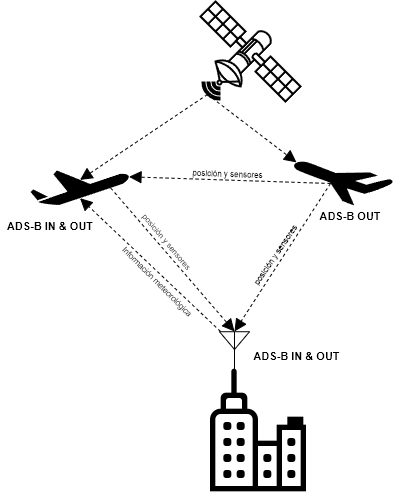
\includegraphics[width=10cm, keepaspectratio]{img/adsbtypes.drawio.png}
	\caption{Ejemplo de tipos de transpondedor ADS-B.}
	\label{fig:adsbtypes}
\end{figure}
\subsection{Contexto y aplicación en el prototipo}
La tecnología \textsc{ADS-B} juega un papel fundamental en el contexto de este proyecto, el objetivo principal del prototipo es la visualización de datos aeronáuticos en un entorno \textsc{\gls{3D}}. Por to tanto esta tecnología nos aporta la capacidad de obtener la información que necesita nuestra aplicación para acceder a los datos que proporcionan dinamismo, ya que las entidades que utilizan esta tecnología estarán constantemente cambiando de posición en el escenario gracias a la variación de los datos de posición.
La tecnología estándar \textsc{ADS-B} nos ofrece una resolución temporal de un segundo entre muestras, aunque los servidores gratuitos normalmente ofrecerán solo la capacidad de acceder a los vectores de información cada cinco segundos como es el caso de \textsc{OpenSky}, resolución suficiente para crear una interpolación entre posiciones y recrear el vuelo de los aviones.
\section{Opensky-network API}
\label{sec:opensky}
\subsection{Introducción a la tecnología}
\textsc{OpenSky} es un proyecto colaborativo de código abierto que permite acceder a la información detallada de las aeronaves gracias a una plataforma o red de sensores distribuida por el mundo recopilando datos en tiempo real sobre el tráfico aéreo.
\subsection{Historia y evolución}
\textsc{OpenSky} se inició sobre los años 2012 cuando un equipo de investigadores de \emph{Armasuisse} (Suiza), la \emph{Universidad de Kaiserslautern} (Alemania) y la \emph{Universidad de Oxford} (Reino Unido) comenzaron a colaborar capturando datos de tráfico aéreo a través de la tecnología \textsc{ADS-B}.
A medida que el proyecto fue creciendo crearon la plataforma online sin ánimo de lucro que hoy conocemos como \textsc{OpenSky Network}, con la finalidad de permitir a los investigadores, desarrolladores y entusiastas de la aviación acceder a los datos que se recopilan.
\subsection{Descripción técnica}
En la red de \textsc{OpenSky} tan pronto como llega un mensaje \textsc{ADS-B} se crea un registro para el avión llamado \emph{vector de estado}.
El vector de estado del servicio contiene la información descrita en la tabla \ref{tab:vectorEstado}.
En la sección \ref{subsec:dao} hablaremos como el prototipo utilizará la \textsc{\gls{API}} proporcionada por los servicios de la organización de software libre \textsc{OpenSky} para consumir datos en tiempo real o en forma diferida a través de una caché local. Esto permitirá crear representaciones en tiempo real del espacio aéreo dentro de un escenario definido por un cuadrado delimitado por coordenadas geodésicas.

\subsection{Contexto y aplicación en el prototipo}
En nuestro caso, utilizaremos la API gratuita que nos brindan los servidores de OpenSky con una resolución temporal de 5 segundos. Por lo tanto, aunque podríamos tener una mayor resolución temporal utilizando la tecnología ADS-B como vimos en la sección \ref{sec:adsb}, nuestra aplicación se adaptará a la opción gratuita que nos ofrece el servicio REST de OpenSky.
\subsection{Ejemplos de uso}
En la figura \ref{fig:getOpensky}, se muestra un ejemplo de una petición GET para las coordenadas de Madrid utilizando la \gls{API} de OpenSky.
En este ejemplo, se realiza una petición \emph{GET} al \emph{endpoint} \emph{https://opensky-network.org/api/states/all} con los parámetros de consulta \emph{lamin}, \emph{lomin}, \emph{lamax} y \emph{lomax} especificados. Además, se incluye un encabezado de autorización con el valor (\emph{Basic user:password}) para autenticar la solicitud donde la parte (\emph{user:password}) puede codificarse en \textsc{Base64} para no ir los datos en claro.
\begin{figure}[h]
	\centering
	\begin{minted}[fontsize=\scriptsize, frame=single, numberblanklines=false,breaklines]{text}
GET /api/states/all?lamin=40.023417&lomin=-4.2041338&lamax=40.7441446&lomax=-3.2538165
Host: opensky-network.org
Authorization: "Basic user:password"
	\end{minted}
	\caption{Petición a la API de OpenSky.}
	\label{fig:getOpensky}
\end{figure}

\begin{table}[h]
	\resizebox{\textwidth}{!}{%
		\begin{tabular}{|c|c|c|c|c|c|}
			\hline
			\textbf{Indice} & \textbf{Propiedad} & \textbf{Tipo} & \textbf{Descripción} \\
			\hline
			0 & icao24 & string & Dirección del transpondedor en hexadecimal. \\
			\hline
			1 & callsign & string & Nombre del avión o vuelo de 8 caracteres. \\
			\hline
			2 & origin\_country & string &  País de origen. \\
			\hline
			3 & time\_position & int & Marca de tiempo UNIX en segundos de la última actualización. \\
			\hline
			4 & last\_contact & int & Marca de tiempo UNIX en segundos de la última trama ADS-B recibida. \\
			\hline
			5 & longitude & float & Coordenada longitud WGS-84. \\
			\hline
			6 & latitude & float & WGS-84 Coordenada latitud WGS-84. \\
			\hline
			7 & baro\_altitude & float & Altitud barométrica en metros. \\
			\hline
			8 & on\_ground & boolean & Indica si la posción se recuperó de un informe de superficie. \\
			\hline
			9 & velocity & float & Velocidad en metros por segundo. \\
			\hline
			10 & true\_track & float & Orientación del avión en grados respector al norte\\
			\hline
			11 & vertical\_rate & float & Velocidad vertical en metros por segundo\\
			\hline
			12 & sensors & int[] & Identificadores de los receptores ADS-B que han contribuido. \\
			\hline
			13 & geo\_altitude & float & Altitud geométrica en metros. \\
			\hline
			14 & squawk & string & Código del transpondedor. \\
			\hline
			15 & spi & boolean & indicador para vuelos de propósito especial. \\
			\hline
			16 & position\_source & int & Fuente del vector de estado. \\
			\hline
			17 & category & int & Enumerado de categoría del avión. \\
			\hline
		\end{tabular}%
	}
	\caption{Vector de estado de la API Rest OpenSky Network.}
	\label{tab:vectorEstado}
\end{table}

\section{HTML5}
\label{sec:html5}
\subsection{Introducción a la tecnología}
\textsc{HTML5} es la última versión del lenguaje de marcado de hipertexto \textsc{HTML}, el lenguaje usado para estructurar y presentar contenido en una web. Junto con la tecnología \textsc{DOM} \ref{sec:dom}, forma la base tecnológica para el desarrollo de aplicaciones web modernas. Mientras que \textsc{HTML5} proporciona las herramientas de marcado para estructura y presentar la información en la web, la tecnologías \textsc{DOM} representa la estructura de ese contenido en forma de árbol de objetos para hacer los datos accesibles y manipulables mediante lenguajes de script.
La combinación de \textsc{HTML5} y \textsc{DOM} permite a los desarrolladores acceder, modificar y actualizar de forma dinámica los elementos y estilos de una página web.
\subsection{Historia y evolución}
En 2004, el \emph{WHATWG}, liderado por Ian Hickson, inició el desarrollo de lo que ahora conocemos como \textsc{HTML5}  Su objetivo principal era mejorar la semántica y estructura del lenguaje \textsc{HTML}, además de agregar nuevas funcionalidades y capacidades para el desarrollo web moderno. El enfoque que resultó exitoso fue el de abordar los problemas y limitaciones que \textsc{HTML} presentaba en ese momento.
Paralelamente, la \textsc{W3C} también estaba trabajando en la evolución de \textsc{HTML}, presentando \textsc{XHTML} como su propuesta. Sin embargo, a medida que el proyecto avanzaba, quedó claro que \textsc{XHTML} no era compatible con el ecosistema web existente.
En 2006, la \textsc{W3C} decidió abandonar el desarrollo de \textsc{XHTML} y unirse al grupo de trabajo \textsc{WHATWG} para colaborar en el desarrollo de \textsc{HTML5}.
Durante el proceso de desarrollo de \textsc{HTML5}, se llevaron a cabo múltiples revisiones y actualizaciones con el fin de incorporar nuevas características, mejorar la semántica, definir \textsc{APIs} y abordar los desafíos técnicos y las necesidades emergentes de la web moderna.

\textsc{HTML5} introdujo una serie de mejoras semánticas,tales como la introducción de los elementos \emph{\textless header\textgreater ,\textless nav\textgreater,\textless section\textgreater, \textless article\textgreater}, entre otros, que permiten una mejor estructuración y accesibilidad del contenido. Además, \textsc{HTML5} incluyó capacidades multimedia nativas mediante la incorporación de elementos como \emph{\textless vídeo\textgreater y \textless audio\textgreater}, lo que eliminó la necesidad de utilizar tecnologías complementarias como \textsc{Flash}.
La especificación de \textsc{HTML5} se finalizó oficialmente en octubre de 2014, marcando un hito importante en la evolución del desarrollo web.
Desde entonces, \textsc{HTML5} se ha convertido en el estándar predominantes para la creación de páginas y aplicaciones web modernas.
\subsection{Descripción técnica}
\textsc{HTML5} se basa en la combinación de las tecnologías \textsc{HTML}, \textsc{CSS} y \textsc{JavaScript} para proporcionar una plataforma de desarrollo web versátil y adaptada a las necesidades modernas. 

\textsc{HTML5} ofrece a los desarrolladores una amplia gama de \textsc{APIs} que les permiten acceder y manipular diversas características del navegador. 
Estas APIs han permitido a los desarrolladores crear experiencias avanzadas como por ejemplo hacer uso de la \gls{API} de geolocalización para obtener la ubicación del usuario y ofrecer servicios personalizados de basados en su posición. Estas herramientas han brindado a los desarrolladores el ecosistema de tecnologías necesarios para el desarrollo de aplicaciones web más sofisticadas.
La \textsc{API} de almacenamiento local permite a las aplicaciones web almacenar datos en el dispositivo del usuario, lo que acelera la experiencia del usuario debido al cacheo de muchos metadatos para mantener estados he incluso poder operar con aplicaciones de manera offline.
Además, \textsc{HTML5} ha introducido nuevas etiquetas semánticas y atributos que permiten una mejor estructuración del contenido y una mayor accesibilidad. Esto facilita a los motores de búsqueda y a los usuarios comprender la información presente en las páginas web de manera más precisa.

Una característica importante que \textsc{HTML5} introdujo en el contexto del proyecto fue la capacidad de crear etiquetas personalizadas. Esta característica permite a los desarrolladores definir sus propias etiquetas \textsc{HTML} para especificar el comportamiento y apariencia utilizando \textsc{JavaScript}.

Esta capacidad de crear etiquetas personalizadas fue aprovechada por los creadores de \textsc{A-Frame} para facilitar la creación de escenas en \textsc{3D}. Utilizando estas etiquetas personalizadas \cite{aframedocs}, los desarrolladores de \textsc{A-Frame} crearon etiquetas que ejecutan el \textsc{JavaScript} necesario para la inicialización de geometrías o componentes de \textsc{Three.js}\cite{threejs}. Esto brinda una forma sencilla y rápida de crear escenas en 3D sin la necesidad de tener un amplio conocimiento de programación 3D, tan solo es necesario definir un \texttt{index.html} usando los elementos creados por la librería para la creación de una escena \textsc{3D}.
\subsection{Contexto y aplicación en el prototipo}
Esta tecnología es la base sobre la cual \textsc{A-Frame} crea la estructura del contenido de realidad virtual en el entorno web. 
Como veremos en la sección \ref{sec:aframe} \textsc{A-Frame} utiliza una combinación de elementos \textsc{HTML5} como \emph{\textless a-scene\textgreater}, \emph{\textless a-entity\textgreater} y \emph{\textless a-camera\textgreater}, junto con componentes propios de \textsc{A-Frame}, para construir y definir objetos \textsc{\gls{3D}}, cámaras, luces y la escena principal.

En resumen, \textsc{A-Frame} utiliza tecnologías como \textsc{HTML5} y componentes propios para definir la jerarquía del escenario y la \gls{renderización} de toda la escena.
\section{DOM}
\label{sec:dom}
\subsection{Introducción a la tecnología}
El \emph{Modelo de Objetos del Documento} conocido como (\textsc{DOM}) es una representación estructurada y jerárquica de un documento \textsc{HTML}, \textsc{XML} o \textsc{XHTML}, que permite acceder y manipular los elementos y contenido del documento mediante programación. Representa la página de manera que los programas puedan cambiar la estructura, estilo y contenido del documento.

El navegador interpreta y construye el \textsc{DOM} a partir del código \textsc{HTML} con el fin de facilitar la manipulación y presentación de la página web. Mediante el uso del \textsc{DOM}, el navegador representa cada elemento del documento \textsc{HTML} como un objeto en la memoria. Este enfoque permite a los desarrolladores web acceder y manipular los elementos, atributos y contenido de la página utilizando lenguajes de programación como \textsc{JavaScript}.

El DOM no es un lenguaje de programación en sí, pero sin él, el lenguaje \textsc{Javascript}~\ref{sec:javascript} no tendría ningún modelo de objetos para una página HTML y sus componentes. El documento en su totalidad, la cabeza, las tablas dentro del documento, los encabezados de tabla, el texto dentro de las celdas de la tabla y todos los demás elementos en un documento son partes del modelo de objetos del documento. Todos ellos pueden ser accedidos y manipulados utilizando el DOM y un lenguaje de scripting como \textsc{JavaScript}.

\subsection{Historia y evolución}
El \textsc{DOM} surgió como un conjunto de objetos que representan a un documento \textsc{HTML} en forma de árbol. Fue creado inicialmente para el navegador \textsc{Netscape} de la compañía \textsc{Netscape Communications}. A partir de mediados de la década de 1990, se convirtió en la interfaz entre el documento \textsc{HTML} y el lenguaje \textsc{JavaScript}~\ref{sec:javascript}, que se incorporó nativamente en los navegadores.

El \textsc{DOM} se originó en respuesta a la necesidad de acceder de manera sencilla a los datos estructurados de los elementos \textsc{XML} y \textsc{HTML}. Proporcionó una manera estándar de manipular y acceder a los elementos, atributos y contenido de un documento web.

Los primeros estándares del \textsc{DOM}, desarrollados por la \textsc{W3C} \emph{(World Wide Web Consortium)}, surgieron como un intento de poner fin a las guerras de los navegadores, donde cada uno ofrecía diferentes técnicas para modificar dinámicamente la estructura de las páginas web. Estos estándares buscaban establecer una forma común y coherente de interactuar con los elementos del documento a través del \textsc{DOM}.
\subsection{Descripción técnica}
El \textsc{DOM} se compone de varios conceptos:
\begin{itemize}
	\item \textbf{\emph{Nodos}}: Son los elementos fundamentales del árbol del \textsc{DOM}. Representan los elementos del documento, y cada nodo, excepto el nodo raíz, tiene un padre. La colección de todos los nodos refleja la jerarquía del documento.
	\item \textbf{\emph{Propiedades y métodos}}: Cada nodo contiene propiedades que representan sus características, como su nombre, atributos, contenido o estilo. Además, los nodos tienen métodos que permiten realizar operaciones sobre ellos, como agregar o eliminar nodos hijos.
	\item \textbf{\emph{Eventos}}: Los nodos del \textsc{DOM} también permiten el manejo de eventos, como cuando el usuario pasa el cursor sobre un nodo o hace clic en él.
	\item \textbf{\emph{Consulta}}: A través de \textsc{JavaScript}, es posible acceder a los elementos del \textsc{DOM} y tener la capacidad de crear, modificar, eliminar y cambiar atributos del \textsc{DOM} de forma dinámica.
\end{itemize}
\subsection{Contexto y aplicación en el prototipo}
Esta tecnología dentro del contexto de la implementación es usada como base para generar entidades y componentes en tiempo real dando el dinamismo a la escena de \textsc{A-Frame}. Es la tecnología usada para que las entidades contenidas en la escena sean manipuladas a través de la modificación de sus propiedades y el envío de eventos.
\subsection{Ejemplos de uso}
Desde cualquier parte del código de nuestra aplicación podemos manipular el \textsc{DOM} a través de los métodos que nos proporciona la \textsc{\gls{API}} de \textsc{Javascript}. Por ejemplo vamos a mostrar como podemos crear un elemento del DOM en nuestra aplicación que representa un avión y agregarlo dentro del elemento que representa la escena:
\begin{minted}[fontsize=\scriptsize, frame=single, numberblanklines=false,breaklines]{javascript}
	function createFlightElement(id) {
		//Vuelo nuevo
		let mainScene = document.querySelector('a-scene');
		let entityEl = document.createElement('a-entity');
		entityEl.setAttribute('id', id);
		entityEl.setAttribute('gltf-model', "#plane");
		entityEl.setAttribute('class', "clickable");
		entityEl.setAttribute('scale', { x: configuration.scale, y: configuration.scale, z: configuration.scale });
		entityEl.setAttribute('hover-scale', 'limitDistance: 100');
		entityEl.addEventListener('mouseenter', evt => handleMouseEnter(evt));
		entityEl.addEventListener('click', evt => handleMouseClick(evt));
		entityEl.addEventListener('mouseleave', evt => handleMouseLeave(evt));
		mainScene.appendChild(entityEl);
		return entityEl;
	}
\end{minted}
\section{JavaScript}
\label{sec:javascript}
\subsection{Introducción a la tecnología}
\textsc{JavaScript} es un lenguaje de programación ampliamente utilizado en el desarrollo web que permite agregar interactividad y dinamismo a las páginas y aplicaciones. Es el único leguaje que permite ser ejecutado en el navegador web de forma nativa, sin necesidad de compilación. Su versatilidad, compatibilidad con \emph{\gls{framework}s} y capacidad para ejecutarse tanto en el lado del cliente como en el lado del servidor lo convierten en una herramienta fundamental para crear experiencias web modernas y funcionales.
\subsection{Historia y evolución}
La historia de \textsc{JavaScript} se remonta a 1995, cuando \emph{Brendan Eich} un programador estadounidense diseñó el lenguaje para \textsc{Netscape Navigator} en un tiempo récord de dos semanas. Inicialmente se llamó \textsc{Mocha} y \textsc{LiveScript}, pero debido  a una colaboración con \textsc{Netscape} y \textsc{Sun} (la empresa propietaria por al quel entonces del lenguaje \textsc{Java}), por cuestiones de marketing ya que \textsc{Java} en aquel entonces era un lenguaje de programación muy popular se decidió establecer como nombre \textsc{JavaScript}.
Sin embargo a pesar de la similitud entre el nombre de \textsc{Java} y el nuevo lenguaje \textsc{JavaScript}, las similitudes entre ambos lenguajes son pocas y no tienen mucho en común.
Al poco tiempo del lanzamiento de \textsc{JavaScript}, \textsc{Microsoft} presentó un lenguaje más o menos compatible llamado \textsc{JScript} para \textsc{Internet Explorer 3.0} .
Para conciliar ambos lenguajes, \textsc{Netscape} presentó \textsc{JavaScript} a la \emph{European Computer Manufacturers Association} (\textsc{\gls{ECMA}}), con el objetivo de crear un estándar que unificase el lenguaje. Fué entonces cuando nació el estándar que se ha denominado \textsc{ECMAScript}, que se adoptó en la versión 6 en 2015 (\textsc{ES6} o \textsc{ES2015} abreviado). Desde entonces se han ido agregando nuevas características año tras año por lo que se acordó no utilizar un número consecutivo de versión, sino simplemente enumerar el año respectivo en el número de versión.
\begin{center}
	\begin{tabular}{|c|c|}
		\hline
		\textbf{Version Name} & \textbf{Year of Publication} \\
		\hline
		ES1 & 1997 \\
		ES2 & 1998 \\
		ES3 & 1999 \\
		ES4 & Not released \\
		ES5 & 2009 \\
		ES6/ES2015 & 2015 \\
		ES2016 & 2016 \\
		ES2017 & 2017 \\
		ES2018 & 2018 \\
		ES2019 & 2019 \\
		ES2020 & 2020 \\
		ES2021 & 2021 \\
		\hline
	\end{tabular}
\end{center}
\subsection{Contexto y aplicación en el prototipo}
En este proyecto \textsc{JavaScript} ha sido el lenguaje de programación base utilizado para la implementación de toda la lógica de negocio desarrollada para el prototipo. Es por lo tanto la herramienta principal para el diseño y desarrollo de componentes que compondrán la escena final . A parte de esto como veremos más adelante es la tecnología sobre la que está construida los \emph{\gls{framework}s} y librerías usados en este proyecto tales como \textsc{A-Frame}~\ref{sec:aframe} y \textsc{Leaflet}~\ref{sec:leaflet}
\subsection{Ejemplos de uso}

\section{WebGL}
\label{sec:webgl}
\subsection{Introducción a la tecnología}
La tecnología de gráficos \textsc{\gls{3D}} es una tecnología que permite la \gls{renderización} de gráficos interactivos en tiempo real sobre un navegador web sin la necesidad de plugins adicionales. Está construida sobre una \textsc{\gls{API}} basada en \textsc{\gls{OpenGL}} para acceder a la funcionalidad de renderizado de la tarjeta gráfica del dispositivo.

WebGL\footnote{\url{https://www.khronos.org/webgl/}} está basada en \textsc{JavaScript}~\ref{sec:javascript} y se relaciona con los elementos de una página web mediante el uso de \textsc{HTML5}~\ref{sec:html5}. 
Proporciona herramientas para crear gráficos \textsc{3D} en el navegador de forma optimizada y eficiente gracias al uso de la \gls{GPU}. \textsc{WebGL} permite una renderización de objetos 3D, texturas, sombreado y efectos visuales avanzados.
\subsection{Contexto y aplicación en el prototipo}
Tanto \textsc{A-Frame} como \textsc{Three.js} utilizan \textsc{WebGL} como tecnología para la renderización de escenas y objetos en \textsc{3D} en un navegador web. Ambas bibliotecas se basan en esta tecnología para realizar operaciones sobre la tarjeta gráfica en el renderizado de sus escenarios.
\section{WebXR}
La tecnología \textsc{WebXR} es una agrupación de estándares que se utilizan en conjunto para habilitar la representación de escenas en 3D en \gls{hardware} diseñado para la visualización de mundos virtuales (VR) o para agregar gráficos al mundo real (realidad aumentada). \textsc{WebXR} proporciona una combinación perfecta entre realidad aumentada y realidad virtual.

Una de las ventajas principales de \textsc{WebXR} es que permite crear experiencias inmersivas directamente en un navegador web gracias a que está construido sobre \textsc{WebGL} \ref{sec:webgl}, sin necesidad de descargar ninguna aplicación adicional. Esto facilita el acceso a estas experiencias a través de múltiples dispositivos, ya que solo se necesita un navegador compatible para disfrutar de ellas.

\textsc{WebXR} proporciona \textsc{\gls{API}} y funcionalidades que permiten interactuar con dispositivos de realidad virtual y realidad aumentada, como gafas \textsc{VR}, cascos \textsc{AR} o incluso dispositivos móviles con capacidades \textsc{AR}. Estas funcionalidades incluyen el seguimiento de la posición y la orientación del dispositivo, renderización de escenas \textsc{3D}, detección de gestos y eventos de interacción, entre otros.

\section{VR}
La realidad virtual (\textsc{VR}) es la tecnología responsable de recrear un entorno ficticio que simula la apariencia real, permitiendo al usuario sumergirse en él y sentir que forma parte de ese entorno. Para experimentar esta realidad virtual, se requieren dispositivos especiales como las gafas o cascos de realidad virtual. Estos dispositivos generan entornos virtuales utilizando la combinación de \gls{hardware} y software diseñados para engañar a nuestros sentidos. Las imágenes en el visor se muestran de manera estereoscópica, lo que significa que se crean dos imágenes ligeramente diferentes para simular una perspectiva diferente en cada ojo. Esto crea una sensación de percepción tridimensional, similar a cómo percibimos el mundo real con nuestros sentidos.
\subsection{Contexto y aplicación en el prototipo}
El prototipo de este proyecto está diseñado para funcionar con dispositivos que generan entornos virtuales, permitiendo una inmersión completa y realista en dicho entorno. Para lograr esto, se utilizan las herramientas proporcionadas por la plataforma A-Frame, como se describe en la sección \ref{sec:aframe}. 
\section{Node JS}
\subsection{Introducción a la tecnología}
\textsc{Node.js} es un entorno de código abierto y multiplataforma que permite la ejecución de código \textsc{JavaScript} de forma asíncrona, con capacidades de entrada y salida de datos, y una arquitectura orientada a eventos. Está basado en el \emph{motor V8} de \textsc{Google} y fue creado con el objetivo de desarrollar programas de red que puedan ser ejecutados en el lado del servidor.

Con \textsc{Node.js}, los desarrolladores pueden construir aplicaciones del lado del servidor utilizando \textsc{JavaScript}, lo que proporciona coherencia en el lenguaje de programación tanto en el lado del cliente como en el servidor. Además, cuenta con una amplia gama de módulos y bibliotecas disponibles a través de su gestor de paquetes \textsc{\gls{npm}}, lo que facilita el desarrollo rápido y eficiente de aplicaciones web y de red.
\subsection{Contexto y aplicación en el prototipo}
Como mencionamos en la sección \ref{subsec:obtencionCache}, hemos utilizado \textsc{Node.js} para desarrollar un \emph{proceso batch} que se encarga de almacenar los datos de la \textsc{API} de \textsc{OpenSky}~\ref{sec:opensky} en una caché local. Esta técnica nos permite ejecutar la aplicación en modo diferido, es decir, obteniendo previamente los datos necesarios y almacenándolos en la caché para su posterior uso.
\subsection{Ejemplos de uso}
A continuación se muestra un ejemplo de código que puede ser ejecutado por \textsc{Node.js} para almacenar los datos obtenidos de la \textsc{API} en un archivo \textsc{\gls{JSON}} para su posterior uso:
\begin{minted}[fontsize=\scriptsize, frame=single, numberblanklines=false,breaklines]{javascript}
	function main() {
		var endpoint = 'https://opensky-network.org/api/states/all?lamin=' + configuration.latMin + '&lomin=' + configuration.longMin + '&lamax=' + configuration.latMax + '&lomax=' + configuration.longMax;
		var credentials = Buffer.from(configuration.apiUser + ':' + configuration.apiPassword).toString('base64');
		setInterval(() => {
			fetch(endpoint, {
				method: 'GET',
				headers: { 'Authorization': 'Basic ' + credentials }
			}).then(response => response.json()).then(json => {
				if (json != undefined && json != null && !isEmptyObject(json)) {
					saveJson(json, index++);
				}
			});
		}, configuration.daoInterval);
	}
\end{minted}
\label{sec:nodejs}
\section{Threejs}
\label{sec:threejs}
\subsection{Introducción a la tecnología}
\textsc{Three.js} es una biblioteca escrita en \textsc{JavaScript} que ofrece una \textsc{API} para interactuar con \textsc{WebGL}~\ref{sec:webgl} y crear de manera sencilla animaciones y escenas \gls{3D} sobre entornos web. 
\textsc{A-Frame}~\ref{sec:aframe} es una de las tecnologías usadas en el prototipo y se basa en \textsc{Three.js} creando una capa de abstracción que simplifica el desarrollo de entornos tridimensionales al permitir el uso directo de \textsc{HTML5}, entidades y componentes. A través de \textsc{A-Frame}, es posible crear escenarios de manera rápida y sencilla, aprovechando la potencia de \textsc{Three.js} en combinación con la facilidad y familiaridad de \textsc{HTML5}.
\subsection{Historia y evolución}
El origen de \textsc{Three.js} se remonta a principios de la década de 2000, cuando el desarrollador \emph{Ricardo Cabello}, también conocido como \emph{Mr.doob}, comenzó a experimentar con gráficos y animaciones en tres dimensiones utilizando tecnologías web. En ese momento, \textsc{WebGL}~\ref{sec:webgl} aún no era muy utilizado y los navegadores no ofrecían un método sencillo para crear contenido \textsc{3D} interactivo.
\emph{Cabello} optó por utilizar la especificación \textsc{WebGL} recién lanzada en 2009, que permitía usar gráficos \textsc{3D} acelerados por \emph{\gls{hardware}} en los navegadores web. Comenzó a trabajar en una biblioteca \textsc{JavaScript} para que los desarrolladores web pudieran crear contenido \textsc{WebGL} más fácilmente.
El proyecto originalmente se llamaba \emph{Canvas 3D} antes de cambiar su nombre a \textsc{Three.js} para reflejar el uso del lenguaje \textsc{JavaScript} como base de la librería.
El objetivo de \textsc{Three.js} era simplificar la programación gráfica en tres dimensiones y facilitar la creación de gráficos interactivos en el navegador.
A medida que más desarrolladores se dieron cuenta de su potencial y comenzaron a usar \textsc{Three.js} en sus proyectos, se hizo rápidamente popular. La creciente adopción de \textsc{WebGL} por parte de los navegadores benefició a la biblioteca, que se convirtió en una herramienta esencial para la creación de contenido \textsc{3D} en la web.
\subsection{Descripción técnica}
Las principales características técnicas de \textsc{Three.js} son las siguientes:
\begin{itemize}
	\item \textbf{\emph{Renderizado en tiempo real}}: aprovechando la aceleración de \emph{\gls{hardware}} proporcionada por \textsc{WebGL}, \textsc{Three.js} es capaz de renderizar gráficos en \textsc{3D} de manera eficiente en los navegadores web modernos.
	\item \textbf{\emph{Geometrías y mallas}}: la biblioteca ofrece una amplia variedad de geometrías predefinidas, como esferas, cilindros, cubos, entre otros. Estas geometrías pueden modificarse mediante atributos, e incluso es posible crear geometrías personalizadas utilizando técnicas de extrusión. Estas geometrías pueden combinarse con mallas para crear superficies y escenas complejas.
	\item \textbf{\emph{Materiales y texturas}}: \textsc{Three.js} proporciona una amplia gama de materiales predefinidos, incluyendo materiales básicos, materiales refractivos, reflectantes y texturas. Estos materiales y texturas se utilizan para agregar detalles a las geometrías y mallas, logrando un mayor realismo en las escenas \textsc{3D}.
	\item \textbf{\emph{Iluminación y sombreado}}: la biblioteca admite diferentes técnicas de iluminación, como luces direccionales, puntuales y de área, lo que permite simular una iluminación realista en la escena. 
	Además, se pueden aplicar técnicas de sombreado suave y sombreado de \emph{Phong} para lograr efectos visuales más sofisticados.
	\item \textbf{\emph{Cámaras y controles}}: \textsc{Three.js} proporciona cámaras que permiten definir la perspectiva y la vista de la escena. Además, incluye controles de cámara predefinidos, como los controles de órbita y los controles de vuelo, que facilitan la interacción del usuario para visualizar la escena \textsc{3D}.
	\item \textbf{\emph{Animaciones}}: \textsc{Three.js} ofrece un sistema de animación que permite crear animaciones de objetos mediante la transición de sus propiedades, como la posición o la escala.
	\item \textbf{\emph{Interactividad}}: \textsc{Three.js} permite la interacción con los objetos de la escena a través de eventos de ratón, teclado y táctiles, lo que brinda una experiencia interactiva al usuario.
\end{itemize}
\subsection{Contexto y aplicación en el prototipo}
\textsc{Three.js} es la librería utilizada por \textsc{A-Frame} como motor gráfico, lo que la convierte en la base para el desarrollo de componentes en el prototipo del proyecto. Además, \textsc{Three.js} se encarga del renderizado en \textsc{3D} y nos brinda las capacidades necesarias para crear componentes que luego pueden ser utilizados con una sintaxis declarativa similar a \textsc{HTML}, a través del uso de \textsc{A-Frame}. 

Por lo tanto, se ha utilizado como tecnología heredada por \textsc{A-Frame}, y los componentes desarrollados en el prototipo hacen uso de la \textsc{API} proporcionada por esta librería.
\subsection{Ejemplos de uso}
En el siguiente ejemplo, podemos apreciar lo sencillo que resulta crear un material y una geometría de tipo línea. Estos serán utilizados para representar en el escenario el trayecto seguido por un vuelo:
\begin{minted}[fontsize=\scriptsize, frame=single, numberblanklines=false,breaklines]{javascript}
	const material = new THREE.LineBasicMaterial({
		color: 0x0000ff,
		linewidth: 1,
		fog: false
	});
	this.geometry = new THREE.BufferGeometry().setFromPoints(this.data.points);
	this.geometry.userData = { points: this.data.points };
	const line = new THREE.Line(this.geometry, material);
	this.el.object3D.add(line);
\end{minted}
\section{A-Frame}
\label{sec:aframe}
\subsection{Introducción a la tecnología}
\textsc{A-Frame}\cite{aframedocs} es un \emph{\gls{framework}} de código abierto construido sobre la tecnología \textsc{Three.js} de la que se habla en la sección\ref{sec:threejs}, que permite la creación de experiencias de realidad virtual en entornos web. A diferencia de otros \emph{\gls{framework}s} \textsc{3D}, \textsc{A-Frame} ofrece un sistema de implementación sencillo, utilizando una sintaxis declarativa similar a la de \textsc{HTML5}. 
Esto facilita a los desarrolladores web la creación rápida e intuitiva de aplicaciones de realidad virtual, sin necesidad de poseer un profundo conocimiento ni adentrarse en la complejidad de la programación en entornos tridimensionales.
Una de las principales ventajas de \textsc{A-Frame} es que se basa en el \emph{modelo entidad componente}, lo que permite el desarrollo de componentes reutilizables y su parametrización para configurar su comportamiento.
Además, \textsc{A-Frame} ya proporciona una amplia gama de geometrías y componentes para la creación de materiales, iluminación, sombras y la gestión de eventos de controladores de realidad virtual, como las gafas \textsc{Oculus}. Esto permite que los proyectos puedan comenzar el desarrollo desde un punto avanzado.

\subsection{Historia y evolución}
\textsc{A-Frame} fue desarrollado por el equipo de \textsc{Mozilla VR} a finales de 2015. Este equipo fue líder en el desarrollo de herramientas para la tecnología \textsc{WebVR}. Debido a la necesidad de crear contenido de manera más sencilla y rápida, se formó un equipo que incluía a los principales mantenedores de este \emph{\gls{framework}}, como \emph{Diego Marcos} y \emph{Josh Carpenter}. 

El objetivo de \textsc{A-Frame} era permitir a los desarrolladores web y diseñadores de experiencias \textsc{3D} y realidad virtual crear contenido utilizando \textsc{HTML}, sin necesidad de tener conocimientos profundos de \textsc{\gls{WebGL}}. El primer lanzamiento público de \textsc{A-Frame} tuvo lugar el 16 de diciembre de 2015. En la actualidad, hay más de 75 contribuyentes en total.
\subsection{Descripción técnica}
Las principales características técnicas de \textsc{A-Frame} son las siguientes:

\begin{itemize}
	\item Configuración de la escena mediante el uso de lenguaje de marcado que nos permite configurar las luces, los controles, las cámaras, los eventos y todo lo relacionado con la configuración \textsc{WebXR}.
	\item Es compatible con la mayor parte de las bibliotecas de desarrollo web basadas en \textsc{JavaScript} como \textsc{React}, \textsc{Angular} o \textsc{Vue}.
	\item Arquitectura entidad-componente favoreciendo la reutilización de componentes complejos.
	\item Contiene una herramienta de inspector visual que se puede invocar desde el navegador mediante la combinación de teclas \texttt{control+alt+i}, ayudando a la depuración y la detección de errores, y permitiendo la visualización de la jerarquía de la escena, consultando sus componentes y permitiendo la modificación de sus atributos.
	\item Proporciona utilidades para optimizar el rendimiento, como es el caso de la función \emph{throttled}, que permite que un código no sea ejecutado en cada refresco de la escena y solo sea ejecutado cada cierto intervalo de tiempo configurado.
	\item Proporciona un componente de animación que permite crear dinamismo de forma sencilla y configurable.
	\item Contiene componentes para los principales controladores de realidad virtual del mercado.
	\item Proporciona primitivas \textsc{HTML5} para las principales geometrías como son planos, cajas, círculos, conos, cilindros, esferas, texto, entre otros.
	\item Gestión de eventos mediante \emph{\gls{raycaster}} que proporciona facilidad de interactuar con las entidades presentes en la escena.
	\item Capacidad de creación de componentes propios o extender alguno existente de manera sencilla e intuitiva.
\end{itemize}

En definitiva, las capacidades técnicas de \textsc{A-Frame} están en continuo crecimiento gracias al gran ecosistema que hay de desarrollo a su alrededor, permitiendo nutrirse también del crecimiento de la tecnología principal, \textsc{Three.js}.
\subsection{Contexto y aplicación en el prototipo}
\textsc{A-Frame} es el motor principal de \emph{renderizado} del prototipo, ya que toda la aplicación está construida haciendo uso de la \textsc{\gls{API}} que proporciona esta librería. Al estar basada en \textsc{JavaScript}, el gestor principal sobrescribe el componente de la escena y define el comportamiento principal de nuestra aplicación mediante el uso de la \textsc{API} de JavaScript en conjunto con los componentes de \textsc{A-Frame} y \textsc{Three.js}.
\subsection{Ejemplos de uso}
\begin{minted}[fontsize=\scriptsize, frame=single, numberblanklines=false,breaklines]{html}
	<html>
	<head>
	<script src="https://aframe.io/releases/1.4.0/aframe.min.js"></script>
	</head>
	<body>
	<a-scene>
	<a-box position="-1 0.5 -3" rotation="0 45 0" color="#4CC3D9"></a-box>
	<a-sphere position="0 1.25 -5" radius="1.25" color="#EF2D5E"></a-sphere>
	<a-cylinder position="1 0.75 -3" radius="0.5" height="1.5" color="#FFC65D"></a-cylinder>
	<a-plane position="0 0 -4" rotation="-90 0 0" width="4" height="4" color="#7BC8A4"></a-plane>
	<a-sky color="#ECECEC"></a-sky>
	</a-scene>
	</body>
	</html>
\end{minted}
\begin{figure}[h]
	\centering
	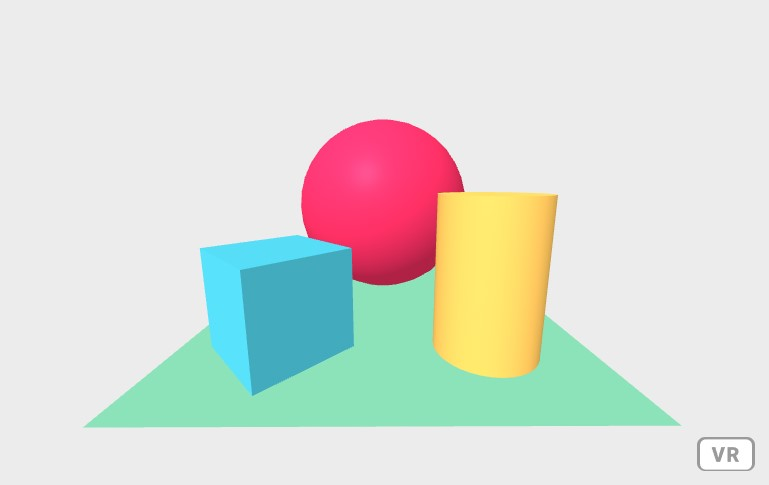
\includegraphics[width=8cm, keepaspectratio]{img/gettingstarted_Aframe.jpg}
	\caption{Escena principal del \emph{Getting Started} de \textsc{A-Frame}.}
	\label{fig:AFrameGettingStarted}
\end{figure}
\section{Leaflet}
\label{sec:leaflet}
\subsection{Introducción a la tecnología}
\textsc{Leaflet} es una biblioteca creada por \emph{Volodymyr Agafonkin} en \textsc{JavaScript} y de código abierto.
Su principal funcionalidad está orientada a la creación de aplicaciones de mapas web. Fue lanzada por primera vez en 2011 y es compatible con la mayoría de las plataformas móviles y de escritorio.
Está tan extendida y es tan liviana que empresas como \textsc{FourSquare}, \textsc{Pinterest} y \textsc{Flickr} la integran dentro de su arquitectura.
\textsc{Leaflet} permite a los desarrolladores mostrar de manera muy sencilla mapas web basados en teselas alojadas en un servidor público. Sobre estos mapas nos permite añadir capas que muestren información creando aplicaciones de manera sencilla y liviana.
\subsection{Contexto y aplicación en el prototipo}
Se ha utilizado esta librería para implementar las conversiones entre coordenadas geodésicas y cartesianas, como se describe en la sección \ref{subsec:mapConversion}. Al utilizar esta librería, nos beneficiamos del soporte técnico que proporciona, asegurándonos de contar con los ajustes necesarios para las fórmulas que desempeñan un papel importante en nuestra aplicación. Además, nos aseguramos de que las conversiones se realicen de la manera más eficiente posible para proporcionar un rendimiento óptimo en entornos móviles.
\subsection{Ejemplos de uso}
A continuación, se presenta un ejemplo de cómo realizamos la conversión de coordenadas geodésicas a cartesianas utilizando la proyección \textsc{Mercator} a través del objeto global \emph{L} que nos proporciona un punto de entrada a las funcionalidades de la librería.
\begin{minted}[fontsize=\scriptsize, frame=single, numberblanklines=false,breaklines]{javascript}
	degreeToMeter(lat, long) {
		let latlng = new L.latLng(lat, long);
		return L.Projection.Mercator.project(latlng);
	}
\end{minted}
\section{GDAL}
\subsection{Introducción a la tecnología}
\textsc{GDAL}\footnote{\url{https://gdal.org/}} es una biblioteca de código abierto que proporciona un conjunto de herramientas para la lectura, escritura y manipulación de datos geoespaciales en diversos formatos. Su desarrollo inicial se centró en facilitar el acceso y procesamiento de datos geoespaciales en diferentes formatos y proyecciones.
Esta biblioteca es ampliamente utilizada en numerosos proyectos que requieren acceder a datos geográficos, como \textsc{Mapserver}\footnote{\url{https://mapserver.org/}}, \textsc{QGIS}\footnote{\url{https://www.qgis.org/es/site/}} y \textsc{GRASS GIS}\footnote{\url{https://grass.osgeo.org/}}. Estas aplicaciones hacen uso de la funcionalidad proporcionada por \textsc{GDAL} para gestionar y visualizar datos geoespaciales de manera efectiva y eficiente.
\subsection{Contexto y aplicación en el prototipo}
Como se explica en la sección \ref{sec:dem}, utilizaremos esta tecnología para llevar a cabo las conversiones de los datos descargados del servidor de \textsc{Copernicus}\footnote{\url{https://land.copernicus.eu/imagery-in-situ/eu-dem/eu-dem-v1.1}}. Estos datos consisten en archivos binarios de alturas, y mediante el uso de esta biblioteca, realizaremos la unión y recorte de una zona específica que representará el terreno de nuestro escenario.

El objetivo es exportar los datos resultantes en el formato binario de alturas requerido por el \emph{componente generador de terrenos}\footnote{\url{https://github.com/bryik/aframe-terrain-model-component}} de la biblioteca \textsc{A-Frame}.
\section{Google Earth Engine}
\subsection{Introducción a la tecnología}
Es una plataforma geográfica basada en la nube que brinda a los usuarios la capacidad de operar, visualizar, analizar y exportar imágenes \gls{raster} de nuestro planeta. Esta plataforma es ampliamente utilizada por científicos y organizaciones sin ánimo de lucro para acceder a información geográfica en forma de datos raster y realizar preprocesamiento y exportación de los mismos.

Los datos geográficos se almacenan en servidores en la nube y se puede acceder a ellos y analizarlos mediante una interfaz de programación de aplicaciones \textsc{API} y un entorno de desarrollo integrado \textsc{IDE} en la nube\footnote{\url{https://code.earthengine.google.com/}}. 
Esta plataforma ofrece a los usuarios una serie de herramientas y funcionalidades que les permiten trabajar con los datos de manera eficiente y precisa.
\subsection{Contexto y aplicación en el prototipo}
Como se mencionará en detalle más adelante en la sección \ref{sec:raster}, esta tecnología se ha utilizado para llevar a cabo la exportación de la capa raster que se utilizará como textura del terreno generado en nuestro escenario. Es importante destacar que esta capa raster estará georreferenciada, lo que permitirá a los usuarios identificar y comprender la ubicación específica en la que se están visualizando los datos dentro del escenario.
La georreferenciación garantiza que el usuario puedan tener una referencia espacial precisa dentro del escenario. Además, las alturas, como montañas o cañones, estarán correctamente posicionadas, lo que proporcionará una sensación realista al visualizar el terreno generado en \textsc{3D}.
\section{Overpass-api}
\subsection{Introducción a la tecnología}
Es una \textsc{\gls{API}} que permite acceder a través de consultas a los datos alojados en los servidores de \textsc{OpenStreetMap}. Utilizando un lenguaje similar al de las bases de datos, podemos filtrar la información y extraer los datos en formato \textsc{XML}. Posteriormente, podemos utilizar herramientas como \textsc{osmtogeojson}\footnote{\url{https://github.com/tyrasd/osmtogeojson}} para convertirlos en archivos \textsc{GEOJSON}, los cuales nuestra aplicación puede aprovechar para representar datos geoespaciales de manera efectiva.
\subsection{Contexto y aplicación en el prototipo}
Como se detalla en la sección \ref{subsec:buildingData}, utilizaremos la página de consultas que nos proporciona la plataforma\footnote{\url{https://overpass-turbo.eu/}} para descargar y procesar los datos de los edificios ubicados en la zona específica de nuestro escenario y alojados en los servidores de \textsc{OpenStreetMap}. Nuestro objetivo será realizar un preprocesamiento de estos datos y subirlos en nuestra aplicación. De esta manera, el prototipo podrá generar las geometrías de los edificios durante la precarga, garantizando así una representación visual precisa de los edificios en el entorno \textsc{\gls{3D}}.
\section{GitHub}
\label{sec:github}
\subsection{Introducción a la tecnología}
\textsc{GitHub} es una plataforma de desarrollo colaborativo basada en la tecnología de control de versiones \textsc{Git}\footnote{\url{https://git-scm.com/}}. Proporciona a los desarrolladores un entorno donde pueden compartir y colaborar en sus proyectos de software de manera eficiente.
Una de las características clave de \textsc{GitHub} es su capacidad para trabajar con ramas. Estas permiten que varios desarrolladores trabajen en diferentes aspectos de un proyecto de forma colaborativa y paralela. Cada desarrollador puede crear su propia rama para trabajar en nuevas funcionalidades, correcciones de errores o mejoras, sin interferir con el trabajo de otros colaboradores. Una vez que los cambios en una rama se consideran estables y completos, pueden fusionarse con la rama principal del proyecto.
\subsection{Contexto y aplicación en el prototipo}
Todo el desarrollo del prototipo de la aplicación \textsc{3D}, incluyendo las demos y los componentes, se encuentra alojado en un repositorio de \textsc{GitHub}\footnote{\url{https://github.com/djprano/AFrameTFG}}. Esta elección se ha realizado con el propósito de mantener un control de versiones y compartir el código fuente del proyecto.
Además también cuenta con la opción de iniciar un servidor de aplicaciones, lo que facilita las demostraciones y la visualización de la aplicación en acción.

\section{VSCode}
\textsc{VSCode} es la herramienta principal que se utiliza como entorno de desarrollo para generar el código del proyecto. Proporciona una variedad de funcionalidades gracias a sus plugins que facilitan el proceso de desarrollo. 
Además, nos permite arrancar un servidor local ligero para ejecutar nuestra aplicación en modo de depuración, lo que nos permite identificar y corregir errores de manera eficiente.
Una de las ventajas de \textsc{VSCode} es su integración con herramientas de control de versiones como la que analizamos en la sección \ref{sec:github}. Además, \textsc{VSCode} ofrece características útiles como autocompletado de código y resaltado de sintaxis, lo que agiliza el desarrollo del prototipo y mejora la productividad.



%%%%%%%%%%%%%%%%%%%%%%%%%%%%%%%%%%%%%%%%%%%%%%%%%%%%%%%%%%%%%%%%%%%%%%%%%%%%%%%%
%%%%%%%%%%%%%%%%%%%%%%%%%%%%%%%%%%%%%%%%%%%%%%%%%%%%%%%%%%%%%%%%%%%%%%%%%%%%%%%%
% DISEÑO E IMPLEMENTACIÓN %
%%%%%%%%%%%%%%%%%%%%%%%%%%%%%%%%%%%%%%%%%%%%%%%%%%%%%%%%%%%%%%%%%%%%%%%%%%%%%%%%

\clearpage

%%%%%%%%%%%%%%%%%%%%%%%%%%%%%%%%%%%%%%%%%%%%%%%%%%%%%%%%%%%%%%%%%%%%%%%%%%%%%%%%
%%%%%%%%%%%%%%%%%%%%%%%%%%%%%%%%%%%%%%%%%%%%%%%%%%%%%%%%%%%%%%%%%%%%%%%%%%%%%%%%
% RESULTADOS %
%%%%%%%%%%%%%%%%%%%%%%%%%%%%%%%%%%%%%%%%%%%%%%%%%%%%%%%%%%%%%%%%%%%%%%%%%%%%%%%%
\chapter{Resultados}
\label{chap:resultados}
\section{Prototipos de demostración}
Podemos acceder y visualizar todas las demostraciones en la página web del proyecto, donde tenemos acceso a demostraciones, videos y escenarios creados utilizando la plataforma del proyecto. Puedes encontrarlos en el siguiente enlace: \url{https://djprano.github.io/AFrameTFG/}.
\subsection{Escritorio}
\subsection{Gafas de realidad virtual}
\subsection{Móvil}
\section{Progreso de desarrollo}
Para modelar el proceso de desarrollo del proyecto, me he basado en la metodología de planificación \textsc{Scrum}.
Esta metodología hace uso de un marco de trabajo ágil, introducido por primera vez en la década de los 90 por \emph{Ken Schwaber} y \emph{Jeff Sutherland} como una herramienta para abordar proyectos complejos.
El enfoque principal de \textsc{Scrum} se fundamenta en la realización de iteraciones incrementales. Esto implica dividir el proyecto en tareas más pequeñas y de corta duración conocidas como \emph{sprints}. 
Cada \emph{sprint} tiene una duración estimada en la cual se llevan a cabo actividades como la planificación, el desarrollo, las pruebas y la revisión.

En el ámbito laboral, es muy común utilizar esta metodología en proyectos tecnológicos, y muchas empresas ofrecen productos para la planificación de proyectos. Uno de los más ampliamente utilizados es \textsc{JIRA}\footnote{\url{https://www.atlassian.com/software/jira}} de \textsc{Atlassian}, que cuenta con una guía de la metodología muy bien documentada \cite{scrumGuide}.

\noindent Algunas de las características que utilizaremos de \emph{Scrum} son las siguientes:
\begin{itemize}
\item \textbf{\emph{Roles}}: se define tres roles principales: \emph{Product Owner} (Dueño del producto), el \emph{Scrum Master} (responsable de que se cumpla la metodología) y el equipo de desarrollo (desarrolladores).
\item \textbf{\emph{Backlog}}: registro de tareas pendientes, que deberán estar estimadas y priorizadas.
\item \textbf{\emph{Artefactos}}: se utiliza varios artefactos para gestionar el trabajo. El más importante es el \emph{Product Backlog}, que es una lista priorizada de todas las funcionalidades, mejoras y tareas pendientes. Otros artefactos incluyen el \emph{Sprint} \emph{Backlog}, que contiene las tareas seleccionadas para el \emph{sprint} actual, y el Incremento, que es la versión funcional del producto al finalizar cada \emph{sprint}.
\item \textbf{\emph{Reuniones}}: la metodología incluye varias reuniones estructuradas para facilitar la colaboración y la toma de decisiones. Estas reuniones incluyen la \emph{Sprint Planning}, donde se define el alcance del \textsc{sprint} actual, la \emph{Daily Scrum}, una breve reunión diaria de seguimiento, y la \emph{Sprint Review}, donde se revisa y se demuestra el trabajo realizado durante el \emph{sprint}.
\end{itemize}

\begin{figure}[h]
  \centering
  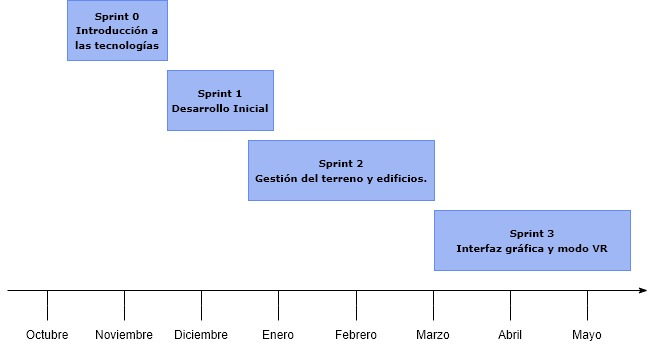
\includegraphics[width=12cm, keepaspectratio]{img/scrum.jpg}
  \caption{Planificación temporal del desarrollo del prototipo.}
  \label{fig:scrum}
\end{figure}

En la figura \ref{fig:scrum} podemos visualizar en el tiempo como se han distribuido las tareas principales. A continuación se presentará una breve introducción de cada uno de los sprints completados en el proyecto:

\begin{itemize}
    \item \textbf{Sprint 0}: En esta etapa, se lleva a cabo una investigación exhaustiva de las tecnologías disponibles para abordar los requisitos del proyecto. Puesta en marcha del entorno de desarrollo y realiza formación para familiarizarse con las librerías y el lenguaje de programación, se realizan experimentos y se busca componentes reutilizables.
    \item \textbf{Sprint 1}: En esta etapa, se sientan las bases para el inicio del prototipo. Se comienza a crear los módulos y componentes que tendrán la funcionalidad principal de mover aviones utilizando datos de \textsc{\gls{API}s}.
    \item \textbf{Sprint 2}: En esta etapa, se enfoca en el desarrollo de la gestión del terreno. Se crea el suelo del escenario con representación realista mediante alturas y texturas. Se desarrollan los módulos encargados del cálculo de alturas y la generación de edificios utilizando datos de \textsc{OpenStreetMaps}.
    \item \textbf{Sprint 3}: En esta etapa, se pone énfasis en la interfaz gráfica. Se crea un ecosistema de componentes reutilizables que permiten al usuario visualizar información, activar y desactivar funcionalidades de la aplicación. Además, se desarrollan los componentes necesarios para la interacción con el escenario, ya sea mediante ratón y teclado o mediante gafas y mandos de realidad virtual.
\end{itemize}

\subsection{Sprint 0}
\subsubsection{Objetivos}
\begin{itemize}
    \item Montar un entorno de programación para aplicaciones web con un servidor liviano para poder arrancar aplicaciones web en local y poder depurar con inspección de variables y puntos de ruptura.
    \item Investigar tecnologías que vamos a necesitar para el desarrollo del prototipo.
    \item Leer documentación de las tecnologías y realizar los ejemplos de la documentación para familiarizarse con la \textsc{API} que nos proporcionan.
    \item Leer libro sobre \textsc{JavaScript} y Documentación para refrescar conocimientos sobre el lenguaje.
\end{itemize}
\subsubsection{Desarrollo}
Se tomó la decisión de utilizar el editor de código \textsc{VSCode} como entorno de desarrollo, debido a la familiaridad previa con esta herramienta en cursos de \textsc{JavaScript}. 
Se instaló \textsc{VSCode} y el servidor de aplicaciones \textsc{Live Server} para ejecutar la aplicación en modo de depuración local.

El uso de la librería \textsc{A-Frame} fue un requisito del \emph{Product Owner}, por lo que se siguieron los ejemplos de la documentación y se realizó el proceso de inicio rápido (\emph{Getting started}).
Se instaló \textsc{Git} y se creó un repositorio en \textsc{GitHub} para mantener un control de versiones y compartir el código fuente del prototipo. 
Además, se configuró un \emph{GitHub Pages} para mostrar la evolución del desarrollo al \emph{Product Owner}.

Se leyó la documentación de \textsc{Three.js} para conocer las herramientas disponibles para futuras implementaciones de componentes de \textsc{A-Frame}.
Se realizó el curso interactivo de \textsc{A-Frame} disponible en \url{https://mozilla.pe/aframe-school/}, lo cual ayudó a resolver muchas dudas y obtener un mejor entendimiento de la tecnología.
Se comenzó a crear animaciones y realizar pruebas con la gestión de eventos del ratón en \textsc{A-Frame}.
Se consultó un \emph{workshop} interesante sobre \textsc{A-Frame} y \textsc{WebXR} en \url{https://github.com/german-alvarez-dev/workshop-webvr-aframe}.

Para abordar el requisito de la creación de un terreno se investigó y se encontraron varios ejemplos de creación de terrenos con \textsc{A-Frame} que podrían ser útiles para el prototipo. 
Algunos de ellos son:
\begin{itemize}
    \item \url{https://github.com/DougReeder/aframe-atoll-terrain}
    \item \url{https://github.com/jesstelford/aframe-map}
    \item \url{https://github.com/bryik/aframe-terrain-model-component}
    \item \url{https://bryik.github.io/aframe-terrain-model-component}
    \item \url{https://github.com/anselm/aterrain}
    \item \url{https://cesium.com/ion}
\end{itemize}
Después de realizar varias pruebas, se concluyó que el componente \emph{aframe-terrain-model-component} era el más adecuado debido a su facilidad de uso y capacidad para manejar archivos \textsc{DEM} en formato \textsc{ENVI}.

Se abordó el requisito de obtener datos de los aviones de una \textsc{API} en línea, y se estudiaron las dos principales opciones de datos \textsc{ADS-B}: \emph{FlightRadar24} y \emph{OpenSky}. Tras evaluar las limitaciones y considerando que \emph{OpenSky} era gratuita y tenía menos restricciones, se decidió utilizar esta \textsc{API}.
Se instala \textsc{Node.js} y se desarrolla un programa simple para probar el servicio web y para almacenar datos localmente y poder trabajar de forma independiente de las limitaciones impuestas por la \textsc{API}.
\subsubsection{Resultado}
Después de realizar todas estas actividades, se llevó a cabo una reunión con el \emph{Product Owner}, quien mostró satisfacción con el progreso y consideró que el equipo estaba listo para abordar el siguiente \emph{sprint}, que implicaría el comienzo del desarrollo del prototipo y cerraría la etapa de investigación de tecnologías.
\subsection{Sprint 1}
\subsubsection{Objetivos}
\begin{itemize}
    \item Desarrollar un módulo que pueda leer los datos locales almacenados por el proceso batch. Además, este módulo debe ser configurable de manera que podamos acceder a datos locales o a datos en tiempo real del servidor.
    \item Encontrar un modelo \textsc{GLTF} de un avión con una licencia que permita su uso y que sea ligero para no afectar el rendimiento. Este modelo debe ser incorporado en la escena y comenzar a posicionarlo en función de los datos \textsc{ADS-B} que se han leído.
    \item Crear animaciones que permitan interpolar linealmente la posición del modelo de avión, evitando cambios bruscos de posición.
    \item Desarrollar un módulo para gestionar la configuración de la escena de manera que se pueda crear aplicaciones para diferentes escenarios utilizando la misma plataforma, simplemente modificando la configuración.
    \item Implementar la capacidad de seleccionar aviones dentro de la escena.
\end{itemize}
\subsubsection{Desarrollo}
Se buscó en la página de \textsc{Sketchfab} un modelo de avión y se encontró un modelo \textsc{GLTF}\footnote{\url{https://sketchfab.com/3d-models/low-poly-plane-151517395bae4d849b30ca53a5e3c5a8}} de uso libre compuesto por tan solo 416 triángulos, el cual se utilizará como icono para los vuelos.
Se creó el componente principal que sobrescribe el comportamiento de la escena principal y actúa como el gestor principal de la aplicación. Para obtener más detalles sobre el diseño de este componente, consulta la sección \ref{sec:mainScene}.
Se realizaron las primeras animaciones de los aviones, pero surgieron algunos problemas. El sistema \textsc{A-Frame} está diseñado para trabajar con unidades en metros. Sin embargo, al utilizar coordenadas absolutas, se encontraron dificultades al manejar posiciones con vectores de dimensiones muy grandes, como el caso del aeropuerto en Madrid, cuyas coordenadas cartesianas son \emph{(-396861, altura, 4937984)}. Estas dimensiones resultan difíciles de manejar. Además, se identificó que uno de los ejes está invertido por el sistema de referencia que posee \textsc{A-Frame}, como se explica detalladamente en la sección \ref{subsec:mapConversion}.
Después de una reunión con el \emph{Product Owner}, se decidió crear un módulo dedicado a gestionar las conversiones entre las coordenadas geodésicas y las coordenadas en el mundo \textsc{\gls{3D}}. En este módulo, se invirtió el eje problemático y se realizó una traslación para centrar el escenario en las coordenadas \emph{(0, 0, 0)}. Además, se aplicó un escalado para manejar distancias en escenarios de grandes dimensiones, como cientos de kilómetros. Todas estas transformaciones se realizaron de manera parametrizada a través de la configuración.
Se comenzaron a crear las primeras animaciones de los aviones con éxito sobre un escenario que representa el aeropuerto de Barajas y sus alrededores. 
También se generaron las primeras siluetas sin extruir en el suelo para comprobar que las posiciones de los aviones coincidían con las posiciones de los edificios, como se muestra en la figura \ref{fig:sprint1}.
Además, se inició la captura de un \emph{\gls{raster}} para incorporar una referencia en forma de mapa de \textsc{OpenStreetMap} en el suelo, lo cual permitirá verificar si se están creando las geometrías en el lugar correcto.
Se implementan en el gestor principal de la escena las primeras interacciones con eventos. Se ha creado una entidad en forma de cono que se posiciona encima del avión para indicar visualmente el avión sobre el cual tenemos el ratón. Esta funcionalidad permite al usuario identificar fácilmente qué avión está siendo seleccionado o resaltado.

\subsubsection{Resultado}
\begin{figure}[h]
  \centering
  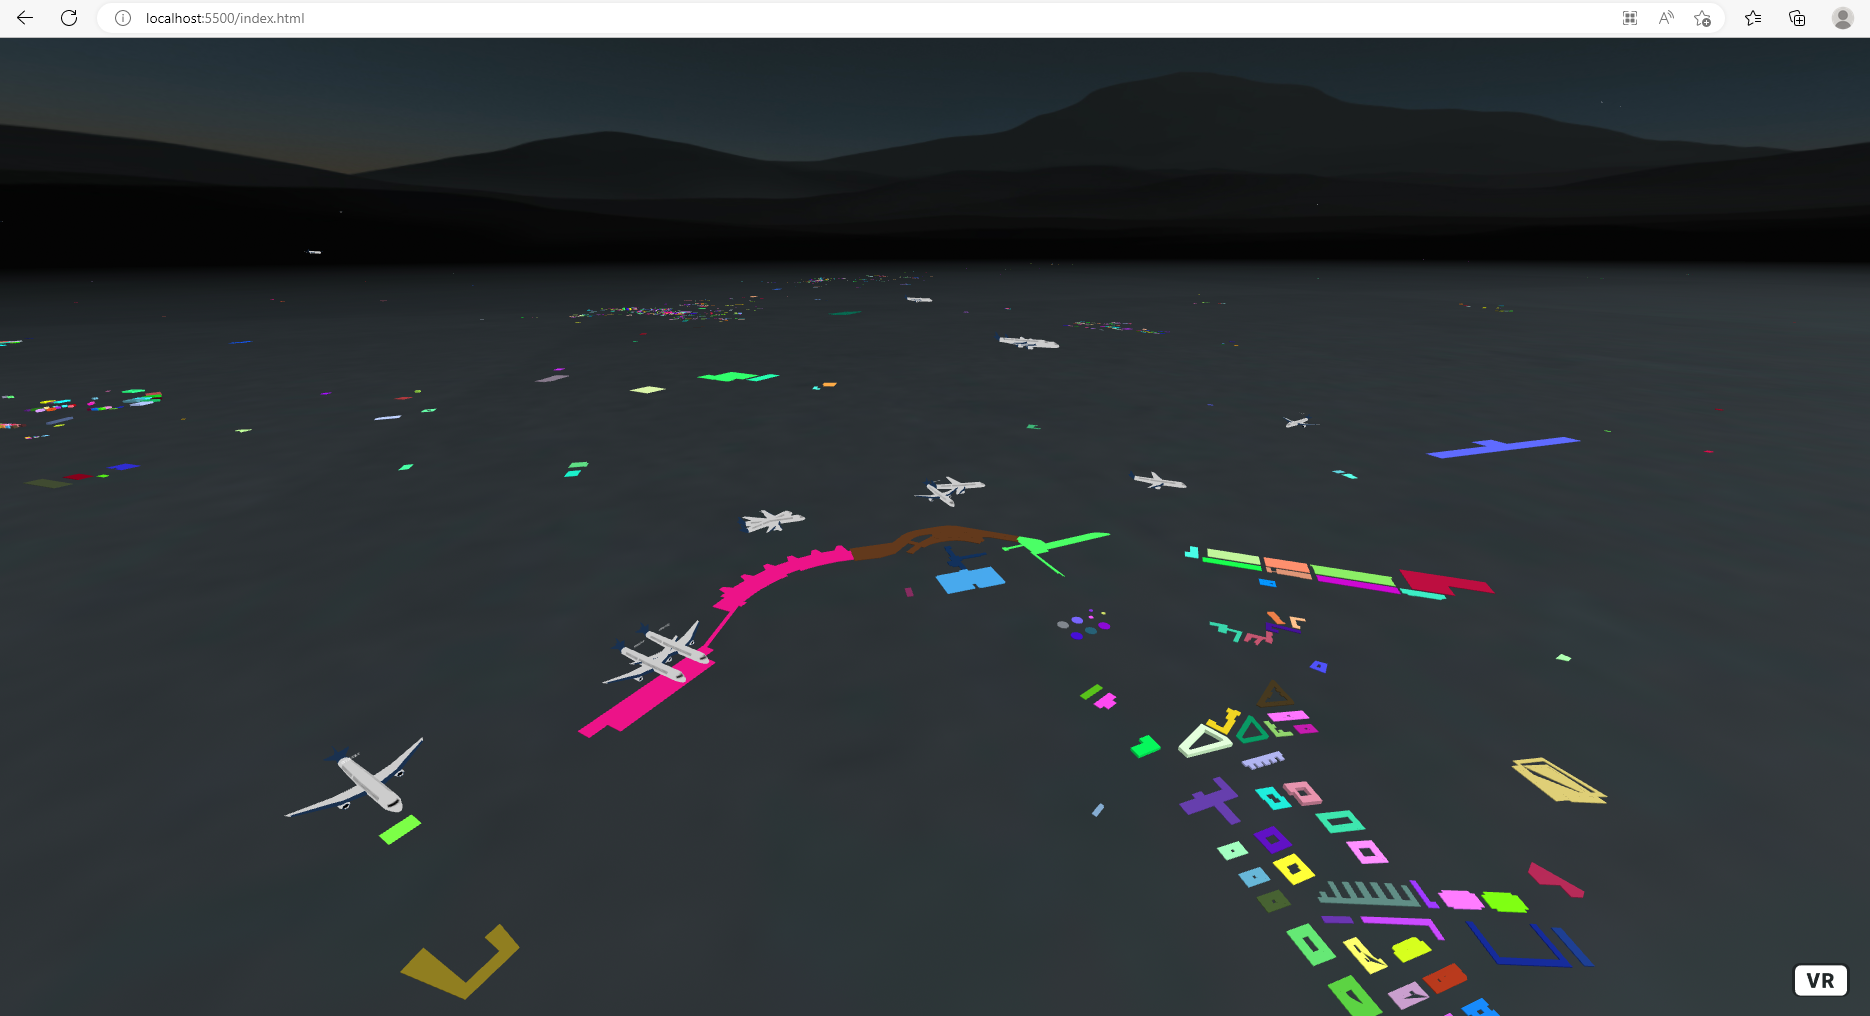
\includegraphics[width=10cm, keepaspectratio]{img/Sprint1.png}
  \caption{Versión inicial.}
  \label{fig:sprint1}
\end{figure}
Durante la reunión final del \emph{sprint} con el \emph{Product Owner}, se ha llegado a la conclusión de que se han cumplido satisfactoriamente los objetivos establecidos. Se considera que se ha logrado una buena base para continuar el desarrollo, especialmente con la incorporación de las siluetas en el terreno de la escena que es parte del desarrollo para el próximo \emph{sprint} donde abordaremos la generación de un módulo que gestiona el terreno.
\subsection{Sprint 2}
\subsubsection{Objetivos}
\begin{itemize}
    \item Generar un archivo \textsc{DEM} y un \emph{\gls{raster}} para los escenarios de Madrid y Vatry.
    \item Integrar en la plataforma el componente \emph{aframe-terrain-model}\footnote{\url{https://github.com/bryik/aframe-terrain-model-component}}, el cual genera un mallado a partir de un archivo binario de alturas.
    \item Desarrollar un módulo para la gestión de terrenos.
    \item Crear un segundo escenario adaptando el gestor de configuración de la aplicación para permitir la cargar toda la plataforma tan solo modificando un fichero en el \textsc{HTML} principal.
    \item Utilizar \textsc{Three.js} para crear geometrías complejas y extruir los edificios en alturas específicas, teniendo en cuenta la altura del terreno.
    \item Adaptar el gestor principal para considerar la altura del terreno al posicionar los aviones.
\end{itemize}
\subsubsection{Desarrollo}
Se generan los ficheros \textsc{DEM} y \emph{\gls{raster}} con éxito siguiendo el procedimiento descrito en las secciones \ref{sec:dem} y \ref{sec:raster}. Para integrar el componente de terrenos en la plataforma, hemos hecho que los parámetros del componente binario de alturas y \emph{raster} del terreno sean configurables, como también la anchura, altura y la magnificación del eje de altura.

Uno de los problemas actuales es que nuestro gestor de alturas debe conocer el valor de altura en cada punto generado por el componente de terreno. Hemos llevado a cabo una investigación consultando el código fuente del componente, y hemos encontrado un evento interno que podemos reutilizar para acceder a la variable de alturas guardada dentro del objeto \textsc{DEM}, como se muestra en la figura \ref{fig:terrain_evento}. Después de ver que los datos almacenados en la variable eran valores extraños e incomprensibles, logramos entender la lógica del \emph{array} de datos. 
El problema residía en que el \emph{array} era del tipo \emph{Uint16Array} y las alturas aplicadas seguían una lógica de normalización del valor del archivo binario multiplicado por el factor de magnificación de alturas. Al insertar esta lógica dentro del nuevo gestor de alturas, realizamos una prueba generando esferas en cada punto del archivo y observamos que se posicionaron correctamente sobre el mallado.
Hemos agrupado toda esta lógica en el archivo \emph{heightManager.js}, que contendrá la instancia única encargada de gestionar la carga del terreno y la \textsc{\gls{API}} de alturas.
Descargamos los datos de edificios y los preprocesamos según se detalla en la sección.\ref{subsec:buildingData} para poder usarlos en el gestor de terreno.

\begin{figure}[h]
  \centering
  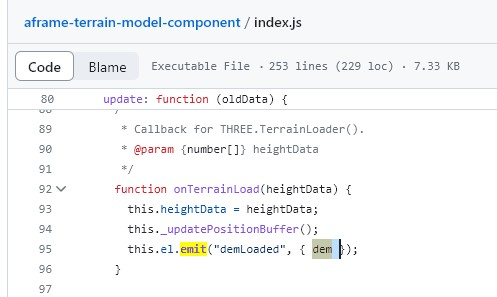
\includegraphics[width=6cm, keepaspectratio]{img/terrain_evento.jpg}
  \caption{Evento clave que emite el componente de terreno.}
  \label{fig:terrain_evento}
\end{figure}
Se realizan todos las modificaciones finales en el modulo de configuración para poder parametrizar la plataforma para otro escenario, y se descargan vuelos, rater y fichero de alturas y edificios tal y como se detalla finalmente en el manual de usuario para generar el escenario de Vatry (Francia) y poner a prueba la versatilidad de la plataforma.
\subsubsection{Resultado}
Podemos observar en la figura \ref{fig:demAframe} como cargamos una demo simple con los ficheros generados del binario de alturas con su respectivo \gls{raster}. 

Se puede visualizar la demo en el siguiente enlace \url{https://djprano.github.io/AFrameTFG/demos/madrid_terrain.html}.
Se realiza la reunión final con el \emph{Product Owner} concluyendo que se han cumplido todos los objetivos cerrando el desarrollo y definiendo los próximos objetivos para el siguiente sprint.
\subsection{Sprint 3}
\subsubsection{Objetivos}
\begin{itemize}
    \item Insertar una geometría que envuelva el cuerpo del avión, indicando cuál está seleccionado y que siempre quede mirando hacia la cámara.
    \item Realizar un panel \textsc{\gls{HUD}} donde visualizar la información de los vuelos seleccionados, refrescándose cuando haya cambios mediante eventos.
    \item Implementar una barra de herramientas para habilitar y deshabilitar funcionalidades.
    \item Encontrar una solución al problema de selección de aviones muy lejanos que son demasiado pequeños.
    \item Almacenar el trayecto que siguen los aviones en una caché desde que entran al escenario y desarrollar una funcionalidad en el \textsc{\gls{HUD}} para visualizar el trayecto.
    \item Insertar una funcionalidad que permita visualizar la perspectiva de lo que se está viendo desde el vuelo.
    \item Permitir al usuario mover el panel \textsc{\gls{HUD}} para colocarlo en una posición donde no le moleste.
    \item Hacer que la aplicación sea compatible con el modo VR y que sea funcional con unas gafas de realidad virtual.
    \item Realizar una implementación que permita al usuario visualizar los metadatos de los edificios.
\end{itemize}
\subsubsection{Desarrollo}
Se crea el componente \textsc{\gls{HUD}} dentro del fichero \emph{hud.js}, el cual va a concentrar toda la lógica del panel de información contextual interactiva y gestión de eventos de selección de aviones, así como la transmisión de información y actualización de los metadatos del vuelo que se visualizan en el panel. 

Finalmente, se decide usar la primitiva \emph{Ring} para rodear al avión seleccionado, tal y como se muestra en la figura \ref{fig:hud}. Para cumplir con el requisito de que siempre mire a cámara, encontramos el componente \emph{look-at}\footnote{\url{https://www.npmjs.com/package/aframe-look-at-component}}, el cual ofrece los resultados esperados, por lo tanto, se decide no realizar ninguna implementación adicional al respecto.

Para el panel contextual, vamos a implementar un panel de \textsc{A-Frame} donde se irán insertando componentes de texto delante, tal y como se detalla en la sección \ref{subsec:hud}. 

Aquí nos topamos con el primer problema en este \emph{sprint}, del cual nos damos cuenta afortunadamente debido a que cuando posicionamos el ratón sobre un elemento de la clase \emph{clickable}, el cursor cambia a una mano. Esto nos hace darnos cuenta de que en ciertas zonas de la pantalla el cursor cambia a mano, pero no hay nada visible que obstaculice la interacción con el elemento. Después de verificar que el panel estaba oculto en la misma zona, llegamos a la conclusión de que el culpable es el panel en modo invisible.

Hemos elegido una estrategia en la que el panel del \textsc{\gls{HUD}} es un elemento \emph{clickable} y, por tanto, intercepta los eventos del \emph{\gls{raycaster}}. Cuando el panel no está visible y está delante del usuario tapando un avión, aunque no vemos que el panel está tapando, al estar invisible, el panel consume los eventos y no podemos seleccionar los aviones.

Solucionamos este problema al posicionar el panel detrás del usuario en lugar de hacerlo invisible. En resumen, cuando el panel recibe el evento de cerrar, se coloca detrás del usuario en una posición donde nunca puede ser visible. De esta manera, deja de interferir en los eventos del controlador principal y podemos seleccionar los objetos sin problemas.
Además, cuando el panel recibe un evento de elemento seleccionado y cambia su posición de oculto a visible, guarda la última posición en la que estaba posicionado antes de recibir el evento de ocultar. De esta manera, cada vez que se oculta el panel, la instancia almacena la última posición para su posterior uso cuando reciba el evento de avión seleccionado.

Desarrollamos una barra de herramientas de dos dimensiones para gestionar la activación y desactivación de funcionalidades. En un principio, esta barra se implementó como un elemento \emph{div} en el \textsc{HTML} principal. Sin embargo, más adelante, cuando probé el prototipo en modo \textsc{VR} utilizando las gafas \textsc{Oculus}, me di cuenta de que los elementos \emph{div} desaparecían en dicho modo.

Por lo tanto, cambiamos nuestra estrategia y comenzamos a desarrollar una solución en la que integraremos una barra de herramientas \textsc{3D} que estará presente como entidades geométricas dentro de la escena, siguiendo la misma filosofía que el \textsc{\gls{HUD}} vease la sección \ref{subsec:toolbar3d}. Esta barra de herramientas contendrá dos botones para activar o desactivar opciones, es decir, serán conmutables, y tendrá un tercer botón cuya función será plegar el panel con una animación para ocupar menos espacio y no interferir en el campo visual del usuario.

En esta etapa del desarrollo, también abordamos otro problema de la aplicación, que es la limitación de seleccionar vuelos que se encuentran demasiado lejos en el escenario. Para resolver esto, desarrollamos un componente llamado \emph{hover-scale}, del cual proporcionamos una descripción técnica en la sección \ref{subsec:hover-scale}. Configuraremos este componente en todas las entidades de aviones, y será responsable de ajustar el factor de escala del avión en función de la distancia con el usuario. De esta manera, cumplimos con el requisito establecido de facilitar al usuario la selección de los vuelos.

Para implementar el requisito de mostrar el trayecto que realiza un avión, creamos un nuevo componente que se agrega a la entidad avión. Este componente se suscribe a los eventos de cambios de posición, y haciendo uso de las ventajas de implementar un \textsc{\gls{DTO}} \emph{(Data Transfert Object)} para manejar el cacheo de los aviones, llamado \emph{FlightCacheData}, insertamos la lógica en este \textsc{DTO} para que cuando se realiza un cambio de posición, envíe un evento. De esta manera, el componente recibe el evento y actualiza la geometría del trayecto. Tan solo tendremos que enviar otro evento desde el panel para visualizarlo, mediante un botón conmutable para mostrar u ocultar el trayecto.

Para ver con más detalle la implementación de esta parte, puedes consultar la sección \ref{subsec:datosCacheVuelo} y la sección \ref{subsec:track}.

Para implementar el requisito de visualizar una perspectiva de cámara a bordo del avión seleccionado, decidimos hacer uso de un artículo y unos componentes disponibles en la guía de introducción de \textsc{A-Frame} de Jesús María González Barahona \cite{aframe_notes}. En esta guía, se explica cómo crear texturas con la visualización de cámaras secundarias.

Haciendo uso del componente \emph{camrender}, cuando el usuario pulsa en el botón conmutable que activa esta opción, creamos una cámara dentro del avión con dicho componente. Luego, utilizando animaciones, creamos un panel al que le asignamos el material de la cámara de a bordo y realizamos una ampliación para crear un efecto de despliegue. Finalmente, colocamos el panel en el \textsc{\gls{HUD}}. De esta forma, implementamos el requisito de visualizar la cámara a bordo de una manera visualmente atractiva, como se muestra en la figura \ref{fig:cameraOnBoard}.

Para el requisito de visualizar los datos de los edificios, se ha desarrollado un componente reutilizable llamado \emph{tooltip-info}. Este componente recibe como argumento un objeto de tipo cadena \emph{String} que se mostrará cuando se reciba un evento de posicionamiento del cursor encima de la entidad correspondiente. Además, el componente modifica el material para indicar cuál es la entidad que se está visualizando, puede consultarse la sección \ref{subsec:tooltip} para más detalle sobre la implementación.

En resumen esta funcionalidad, al crear los edificios, se procesan los metadatos provenientes de la información de \textsc{OpenStreetMap}. Se genera una cadena de texto que se pasa como parámetro al componente \emph{tooltip-info}, asignándolo a la entidad correspondiente. El componente \emph{tooltip-info} calcula la posición más alta de la geometría del edificio y crea un texto que se muestra de manera visible y siempre mirando hacia la cámara cuando el cursor se posiciona encima del edificio.

El último desafío al que nos enfrentamos fue el de mover las entidades \textsc{\gls{HUD}} que existen dentro de la estructura del usuario, ya sea a través del ratón o de los controladores de realidad virtual de las gafas \textsc{Oculus} que nos proporcionó el universidad. En un principio, consideramos utilizar el componente \emph{aframe-super-hands-component}\footnote{\url{https://github.com/c-frame/aframe-super-hands-component}}, ya que es ampliamente utilizado en la comunidad de desarrollo de \textsc{A-Frame}. Comenzamos a integrar este componente en nuestro prototipo, pero resultó ser un fracaso. Los movimientos solo funcionaban cuando la cámara miraba en una dirección, y a medida que se movía la cámara, los movimientos se volvían incoherentes.

Después de investigar el código fuente de la biblioteca, llegamos a la conclusión de que el componente no era adecuado para nuestro caso, ya que estábamos intentando mover una entidad que no tiene coordenadas absolutas, sino coordenadas relativas a la cámara. 
Además, los componentes \emph{movement-controls} establecidos en la entidad \emph{Rig} en combinación con el componente \emph{look-controls} en la cámara hacían que las posiciones relativas de la cámara tampoco fueran absolutas. También debíamos asegurarnos de que al arrastrar una entidad, no moviéramos la cámara, ya que el movimiento natural del ratón se utiliza para desplazar la orientación cámara.

Para solucionar este requisito, implementamos un componente personalizado que tuviera en cuenta todas estas peculiaridades y nos permitiera arrastrar objetos ubicados jerárquicamente dentro de la entidad de la cámara. También, para evitar la rotación de la cámara mientras se arrastra una entidad, deshabilitamos el componente \emph{look-controls} mientras se está realizando el arrastre del elemento \textsc{\gls{HUD}}.

Para obtener más detalles sobre cómo se implementó este componente \emph{custom-draggable} , consulta la sección \ref{subsec:customDraggable}.

\subsubsection{Resultado}
Se lleva a cabo una reunión final con el \emph{Product Owner} para mostrarle el prototipo y se finalizan todos los desarrollos, cumpliendo con los requisitos establecidos en este \emph{sprint}. Posteriormente, se procede a cerrar las etapas de desarrollo con el objetivo de completar la documentación final. 

\section{Construcción de escenas}
Aquí presentaremos un resumen del procedimiento necesario para crear un escenario y configurar la plataforma proporcionada por el prototipo. Además, en la sección \ref{sec:componentesreutilizables}, describiremos los componentes que se pueden reutilizar en otros proyectos y cómo hacerlo.

\subsection{Generación de datos para el terreno}
El primer paso consiste en determinar las coordenadas geodésicas para nuestro escenario. Es importante intentar definir un rectángulo con coordenadas que formen un plano lo más cuadrado posible. Esto se debe a que, aunque el cálculo se basa en ambas dimensiones, la cúpula del cielo se construye utilizando la coordenada más corta para asegurarse de que no tengamos una parte del área sin cubrir en el horizonte. 
Un escenario con proporciones cuadradas evitará tener un exceso de terreno fuera de la cúpula, lo cual podría afectar al rendimiento. En resumen, se recomienda generar coordenadas cuadradas en la medida de lo posible.
Una vez que tengamos las coordenadas geodésicas de nuestro escenario, procederemos a extraer el archivo \textsc{DEM} (Modelo de Elevación Digital) y el archivo \gls{raster} para configurar correctamente los archivos necesarios para crear el terreno. A continuación, seguiremos los pasos enumerados en el manual \ref{manual:generacionDem} para generar un archivo binario de alturas basado en las coordenadas seleccionadas. Para la generación del archivo raster, utilizaremos el script proporcionado en la figura \ref{manual:generacionRaster}, el cual se basa en el servicio de \textsc{Google} \cite{googleearthengine}. Asegúrate de reemplazar las coordenadas establecidas en el script con las correspondientes a tu escenario.

\subsection{Generación de edificios para el terreno}
El siguiente paso consiste en generar los edificios que queremos que aparezcan dentro de nuestro escenario. Para ello, seguiremos estos pasos:

\begin{enumerate}
	\item Utilizando el \emph{endpoint} \ref{manual:consultaEdificios} y sustituyendo las coordenadas por las del escenario, descargaremos los metadatos del servidor de \textsc{OpenStreetMaps} en formato \emph{OSM}. Esta consulta se puede realizar desde el Navegador o utilizando un software para hacer peticiones, como \textsc{POSTMAN}, que nos permita guardar el resultado de la consulta. Es importante tener en cuenta que el tamaño del archivo dependerá del escenario, y si se trata de una zona con muchos edificios, podría llegar a pesar cientos de \emph{Megabytes}. 
	
	Para evitar problemas de rendimiento en la aplicación, se recomienda aplicar algún tipo de filtrado adicional para obtener una lista reducida de edificios.
	\item El siguiente paso consiste en procesar el archivo para generar un formato de archivo \textsc{GeoJSON} compatible con nuestra plataforma. Para ello, podemos instalar la librería \textsc{osmtogeojson} utilizando \emph{\gls{npm}} y ejecutar el comando en la consola, tal como se indica en el script \ref{manual:osmtogeojson}.
\end{enumerate}
\subsection{Almacenar metadatos de vuelos dentro del escenario (Opcional)}
El siguiente paso es necesario solo en caso de que deseemos ejecutar el escenario en modo \emph{offline} (sin conexión). Siempre que queramos utilizar la aplicación en modo tiempo real, este paso puede omitirse.
Si deseamos levantar la aplicación en modo \emph{offline}, es necesario contar con un archivo de vectores de posición de vuelos guardados en una carpeta configurada. Para guardar los datos de vuelos para las coordenadas del escenario, ejecutaremos el proceso por lotes \emph{openSkyDataSaver.js}. En la sección \ref{subsec:obtencionCache}, se describe el proceso realizado, pero veamos más detalles a continuación.

Debemos crear un archivo principal que cargue la configuración necesaria para ejecutar el proceso por lotes y que llame al método principal de la clase para inicializar el proceso. En la siguiente figura se muestra un ejemplo explicado con comentarios en las lineas principales.
\begin{minted}[fontsize=\scriptsize, frame=single, numberblanklines=false,breaklines]{javascript}
	import * as configuration from "./configuration/configurationModel.js";
	import * as openSkyDataSaver from "./openSkyDataSaver.js";
	
	//Establecemos las coordenadas del escenario.
	configuration.setMerConfig(40.0234170,40.7441446,-4.2041338,-3.2538165);
	//Ruta absoluta a la carpeta donde queremos almacenar los datos de vuelo
	configuration.setFlightLocalFolder('C:\\Users\\djpra\\Documentos\\workspaceTFG\\........');
	//Usuario de la API OpenSky si no se posee uno simplemente hay que registrarse.
	configuration.setApiUsuer('xxxxxx');
	//Contraseña de la web OpenSky.
	configuration.setApiPassword('xxxxxxx');
	//Intervalo entre peticiones, recordar que gratuitamente nos e permite vectores de posición menos a 5seg.
	configuration.setDaoInterval(5100);
	//Lanzamos el proceso.
	openSkyDataSaver.main();
}
\end{minted}

Después para lanzar el proceso por lotes simplemente ejecutar el siguiente comando en consola contra el fichero anteriormente explicado:
{\scriptsize
\begin{verbatim}
	node ficheroPrincipal.js
\end{verbatim}
}

\subsection{Generación de fichero de configuración}
\label{conf:ficheroConfig}
Ahora vamos a crear un archivo de configuración en formato \emph{JavaScript} donde estableceremos todos los parámetros de nuestra plataforma. 
A continuación, se muestra un ejemplo detallado con cada uno de los parámetros:
\begin{minted}[fontsize=\scriptsize, frame=single, numberblanklines=false,breaklines]{javascript}
import * as configuration from "./configurationModel.js";
//Coordenadas del escenario latmin, latmax, longmin, longmax.
configuration.setMerConfig(40.0234170,40.7441446,-4.2041338,-3.2538165);
//Coordenadas de la posición inicial del usuario.
configuration.setCamPosition(40.4893, -3.52254);
//Nombre del fichero de edificios sin extensión ubicado en la carpeta 
//"data" del proyecto.
configuration.setBuildingFileName('madrid_building');
//sufijo de la carpeta que contiene los vuelos, debe contener el prefijo "flightData"
//Opcional solo para uso offline.
configuration.setFlightLocalFolder('_madrid');
//fichero con la capa raster del terreno ubicado en la carpeta 
//"data" del proyecto.
configuration.setMapRaster('Madrid_raster.jpg');
//fichero binario de alturas para el terreno ubicado en la carpeta 
//"data" del proyecto.
configuration.setMapDem('madrid_dem.bin');
//Establece si queremos lanzar la aplicación en modo offline con los datos de la carpeta
//caché.
configuration.setLocalApiMode(true);
//Intervalo de refresco de los datos, cada cuanto se realiza una petición.
configuration.setDaoInterval(2000);
//En caso de modo offline por cual fichero queremos empezar la reproducción.
configuration.setDaoLocalIndex(0);
//Usuario de la API OpenSky si no se posee uno simplemente hay que registrarse.
configuration.setApiUsuer('xxxx');
//Contraseña de la web OpenSky.
configuration.setApiPassword('xxxxx');
\end{minted}
Es fundamental tener identificado este archivo, ya que será el que especificaremos en el cuerpo de nuestro archivo \emph{index.html} para ejecutar la configuración de nuestra aplicación.
\subsection{Creación de la página principal de nuestra aplicación}
En esta sección, crearemos la página principal que iniciará nuestra aplicación. Esta página solo varía en función del escenario seleccionado y del archivo de configuración que se cargue. Por lo tanto, solo necesitamos copiar la estructura principal del archivo \emph{index.html}, como se muestra a continuación. 
En la línea 20 donde se encuentra \emph{configuraciónEscenario.js}, debemos establecer la ruta al archivo de configuración que creamos en la sección anterior \ref{conf:ficheroConfig}. 
A continuación, se muestra la estructura genérica de la página principal de nuestra aplicación:
\label{conf:index}
\begin{minted}[fontsize=\scriptsize, frame=single, numberblanklines=false, linenos=true, breaklines]{html}
<!DOCTYPE html>
<html lang="es">

<head>
<meta charset="UTF-8" />
<meta name="viewport" content="width=device-width, initial-scale=1" />
<title>Vatry</title>
<link rel="stylesheet" type="text/css" href="css/aframe.css">

<script src="https://aframe.io/releases/1.4.0/aframe.min.js"></script>
<script src="https://cdn.jsdelivr.net/gh/c-frame/aframe-extras@7.0.0/dist/
aframe-extras.min.js">
</script>
<script
src="https://unpkg.com/aframe-terrain-model-component@1.0.1/dist/
aframe-terrain-model-component.min.js"></script>
<script src="https://unpkg.com/aframe-look-at-component@0.8.0/dist/
aframe-look-at-component.min.js"></script>
<script src="https://unpkg.com/leaflet@1.9.2/dist/leaflet.js"
integrity="sha256-o9N1jGDZrf5tS+Ft4gbIK7mYMipq9lqpVJ91xHSyKhg=" crossorigin=""></script>
<script src="js/configuration/configurationModel.js" type="module"></script>
<script src="js/configuration/configuraciónEscenario.js" type="module"></script>
<script src="js/gui/hud.js" type="module"></script>
<script src="js/gui/custom-draggable.js" type="module"></script>
<script src="js/gui/hover-scale.js" type="module"></script>
<script src="js/map-ground/building-geometry.js" type="module"></script>
<script src="js/mainscene.js" type="module"></script>
<script src="js/map-ground/camera-height.js" type="module"></script>
<script src="js/gui/oculus-test.js" type="module"></script>
<script src="js/gui/tooltip-info.js" type="module"></script>
<script src="js/gui/toolbar3d.js" type="module"></script>
<script src="js/gui/track.js"></script>
<script src="js/gui/camrender.js"></script>
<script src="js/gui/canvas-updater.js"></script>

</head>

<body>
<a-scene main-scene>
<a-assets>
<img crossorigin="anonymous" id="skyImage" src="https://cdn.aframe.io/a-painter/images/sky.jpg">
<img crossorigin="anonymous" id="groundTexture" src="data/vatry_map.png">
<a-asset-item id="plane" src="plane/scene.gltf"></a-asset-item>
<canvas id="cameraOnBoard"></canvas>
</a-assets>
<!-- Camera -->
<a-entity id="rig" position="0 0 0" movement-controls terrain-height>
<a-entity id="camera" hud camera look-controls="reverseMouseDrag:false" cursor="rayOrigin: mouse; fuse: false"
raycaster="far: 4000; objects: .clickable" position="0 0 0" toolbar3d>
</a-entity>
<a-entity id="left-hand" oculus-touch-controls="hand: left" laser-controls="hand: left"
raycaster="far: 4000; objects: .clickable"></a-entity>
<a-entity id="right-hand" oculus-touch-controls="hand: right" laser-controls="hand: right"
raycaster="far: 4000; objects: .clickable"></a-entity>
<a-entity id="cameraOnBoarEntity" camera="active: false" camrender="cid:cameraOnBoard;fps:25" position="0 0 0"
rotation="0 -180 0"></a-entity>
</a-entity>
<a-sky id="sky" src="#skyImage" theta-length="90" radius="1000"></a-sky>

<a-sphere id="moon" material="shader: flat; color: #fef7ec" radius="10" position="-96 350 -238"
light="type: directional; color: #fef7ec; intensity: 0.65"></a-sphere>

<a-entity light="type: ambient; color: #fef7ec; intensity: 0.3" position="0 0 300"></a-entity>
</a-scene>
</body>

</html>
\end{minted}

\section{Componentes reutilizables}
\label{sec:componentesreutilizables}
En esta sección, se presentarán en detalle los componentes de la aplicación que pueden ser reutilizados en otros proyectos a través de la configuración. Además, se presentarán aquellos componentes que pueden integrarse en otros proyectos a través de pequeñas modificaciones. También se incluirán instrucciones detalladas sobre cómo llevar a cabo la reutilización de estos componentes.
\subsection{Componente de Información Contextual Interactiva}
Este componente tiene la función de mostrar información contextual sobre una entidad específica. Permite al usuario obtener detalles adicionales o aclaraciones sobre el elemento seleccionado. Si deseas obtener más información sobre cómo implementarlo y utilizarlo, te recomiendo consultar la sección \ref{subsec:tooltip} donde se brindarán más detalles al respecto.
\subsubsection{ruta}
{\scriptsize
	\url{https://github.com/djprano/AFrameTFG/blob/main/js/gui/tooltip-info.js}
}

\subsubsection{Guía del programador}
\label{subsub:clickable}
Para que este componente funcione es un requisito que la entidad sea de la clase \emph{clickable} por lo tanto , debes establecer la clase de la siguiente forma:
{\scriptsize
	\begin{verbatim}
		entidadEl.setAttribute('class', "clickable");
	\end{verbatim}
}
Después simplemente debes calcular el literal que quieres establecer como texto contextual para la entidad y pasarlo como argumento del componente cuando se configura en la entidad.
\subsubsection{Ejemplo de uso}
{\scriptsize
	\begin{verbatim}
		entidadEl.setAttribute('tooltip-info', { info: "Texto contextual" });
	\end{verbatim}
}

\subsection{Componente arrastrar entidades HUD}
En esta sección hablaremos del componente que permite al usuario cambiar de posición una entidad relativa a la cámara , moviendose a lo largo de un plano perpendicular a la cámara es decir que no permite arrastrar la entidad en la dimensión de profundidad solo en altura y anchura. 
\subsubsection{ruta}
{\scriptsize
	\url{https://github.com/djprano/AFrameTFG/blob/main/js/gui/custom-draggable.js}
}
\subsubsection{Guía del programador}
Para asegurarnos de poder interactuar con todos los componentes mediante eventos del ratón o del controlador de las gafas de realidad virtual, es necesario que la entidad en la que vamos a configurar este componente sea de la clase \emph{clickable} (vease  \ref{subsub:clickable} para obtener más detalles al respecto).
Además, otro requisito importante que mencionamos previamente en la descripción, pero es necesario resaltarlo, es que este componente está diseñado específicamente para mover o arrastrar entidades en altura o anchura, pero no en profundidad. Además, estas entidades deben estar ubicadas dentro de la jerarquía de la cámara.
Por último, es recomendable configurar el componente \emph{look-at}\footnote{\url{https://www.npmjs.com/package/aframe-look-at-component}} en la entidad que vamos a mover. Esto permitirá que la entidad siempre se oriente hacia la cámara.
\subsubsection{Ejemplo de uso}
{\scriptsize
	\begin{verbatim}
		//Establecemos la clase clickable
		hudEl.setAttribute('class', "clickable");
		//Configuramos el componente look-at para que mire al elemento camera
		hudEl.setAttribute('look-at', '#camera');
		//Configuramos el componente que nos permite desplazar la entidad con los controladores
		hudEl.setAttribute('custom-draggable', '');
	\end{verbatim}
}
\subsection{Componente barra de herramientas 3D}
En esta sección vamos a detallar como reutilizar el componente de barra de herramientas que junto con el componente \emph{custom-draggable} del que hablamos en la sección anterior proporciona un elemento en el mundo de realidad virtual con botones conmutables que viajan con la cámara permitiendo activar o desactivar funcionalidades de la aplicación al usuario.
\subsubsection{ruta}
{\scriptsize
	\url{https://github.com/djprano/AFrameTFG/blob/main/js/gui/toolbar3d.js}
}
\subsubsection{Guía del programador}
\label{subsec:guiaBarra3d}
Para reutilizar este componente, es necesario agregarlo a la entidad de la cámara. Se trata de un componente diseñado para viajar con la cámara y añadir una superficie desplazable que proporciona botones con funcionalidades para la aplicación.
Para ello, puedes crear un componente que herede del código existente y sobrescribir el método \texttt{init}. También es posible copiar el código y simplemente definir tu propio método \texttt{init}.

Dentro de este método, debes añadir los botones y establecer su funcionalidad. Para crear un botón, utiliza la función interna llamada \texttt{createToolbarButton}, la cual recibe los siguientes parámetros:

\begin{itemize}
	\item \textbf{\emph{id}}: Identificador del elemento que se va a crear.
	\item \textbf{\emph{widht}}: Ancho del botón en unidades del mundo 3D.
	\item \textbf{\emph{hight}}: Alto del botón en unidades del mundo 3D.
	\item \textbf{\emph{deep}}: Grosor del botón en unidades del mundo 3D.
	\item \textbf{\emph{text}}: Texto del botón en caso de ser pulsable.
	\item \textbf{\emph{texSize}}: Tamaño de la letra del botón en unidades del mundo 3D.
	\item \textbf{\emph{position}}: Vector de posición relativa al panel de la barra de herramientas.
	\item \textbf{\emph{tooble}}: Booleano que indica si es un botón conmutable.
	\item \textbf{\emph{enableFucntion}}: Función que se ejecuta cuando el botón conmutable es activado.
	\item \textbf{\emph{disableFunction}}: Función que se ejecuta cuando el botón conmutable es desactivado.
	\item \textbf{\emph{enableColor}}: Color del botón conmutable cuando está activado.
	\item \textbf{\emph{disableColor}}: Color del botón conmutable cuando está desactivado.
	\item \textbf{\emph{enableText}}: Texto del botón conmutable cuando está activado.
	\item \textbf{\emph{disableText}}: Texto del botón conmutable cuando está desactivado.
\end{itemize}

De esta manera, al crear los botones con su funcionalidad y agregar este componente dentro de la cámara, obtendremos una barra de herramientas en la aplicación que se necesite.
\subsubsection{Ejemplo de uso}
A continuación mostramos un ejemplo para la creación de un botón:
\begin{minted}[fontsize=\scriptsize, frame=single, numberblanklines=false, breaklines]{javascript}
	//Creamos un botón para habilitar el hud
	this.hudEnableButton = this.createToolbarButton('hudEnableButton',0.3, 0.15, null,null, { x: -0.09, y: 0, z: 0.06 }, true,
	() => this.sceneEl.emit('hud-enable', null),
	() => this.sceneEl.emit('hud-disable', null),
	'#0a0', '#a00', 'Hud enable', 'Hud disable');
	this.toolbar.appendChild(this.hudEnableButton);
\end{minted}

Para agregar el componente, tan solo debemos configurar \emph{toolbar3d} dentro del elemento cámara como podemos ver en el siguiente ejemplo:
\begin{minted}[fontsize=\scriptsize, frame=single, numberblanklines=false, breaklines]{html}
	<a-entity id="camera" hud camera look-controls="reverseMouseDrag:false" cursor="rayOrigin: mouse; fuse: false"
	raycaster="far: 4000; objects: .clickable" position="0 0 0" toolbar3d>
\end{minted}
\subsection{Geometría edificio}
El siguiente componente es una implementación personalizada de geometría en \textsc{Three.js}, diseñado específicamente para representar edificios utilizando las coordenadas de su contorno. Este componente se encarga de extruir el contorno proporcionado y realizar las transformaciones afines necesarias para posicionar la geometría en el lugar correcto en la escena tridimensional.
Este componente personalizado resulta especialmente útil para proyectos que involucren la visualización de edificios y estructuras arquitectónicas en entornos 3D.
\subsubsection{ruta}
{\scriptsize
	\url{https://github.com/djprano/AFrameTFG/blob/main/js/map-ground/building-geometry.js}
}
\subsubsection{Guía del programador}
Para usar esta geometría necesitamos pasarle los siguientes parámetros:
\begin{itemize}
	\item \textbf{points}: Lista de puntos en coordenadas 2D que definen las posiciones X y Z del contorno donde vamos a dibujar el edificio.
	\item \textbf{terrainHeight}: Altura del terreno, donde se asienta la geometría del edificio.
	\item \textbf{height}: Altura del edificio.
\end{itemize}
Con estos datos y creando una entidad con la primitiva está geometría se creará un edificio en el escenario.
\subsubsection{Ejemplo de uso}
\begin{minted}[fontsize=\scriptsize, frame=single, numberblanklines=false, breaklines]{javascript}
	let wayPoints = [];
	wayPoints.push({ x: 0, y: 1 });
	wayPoints.push({ x: 1, y: 1 });
	wayPoints.push({ x: 1, y: 0 });
	wayPoints.push({ x: 0, y: 1 });
	let buildingProperties = { primitive: "building", points: wayPoints, terrainHeight: 0 , height:20};
	let item = document.createElement("a-entity");
	item.setAttribute("geometry", buildingProperties);
	item.setAttribute("material", { color: '#88e9fd', roughness: 0.8, metalness: 0.5 });
	
\end{minted}


%%%%%%%%%%%%%%%%%%%%%%%%%%%%%%%%%%%%%%%%%%%%%%%%%%%%%%%%%%%%%%%%%%%%%%%%%%%%%%%%
%%%%%%%%%%%%%%%%%%%%%%%%%%%%%%%%%%%%%%%%%%%%%%%%%%%%%%%%%%%%%%%%%%%%%%%%%%%%%%%%
% CONCLUSIONES %
%%%%%%%%%%%%%%%%%%%%%%%%%%%%%%%%%%%%%%%%%%%%%%%%%%%%%%%%%%%%%%%%%%%%%%%%%%%%%%%%

\clearpage


\chapter{Diseño e implementación}
\label{sec:diseno}
\section{Arquitectura general de la aplicación} 
\label{sec:arquitectura}
Se ha diseñado una arquitectura modular tal y como podemos ver en la figura~\ref{fig:arquitectura}, donde se ha dividido la lógica de la aplicación en distintos ficheros que se han organizado por responsabilidad a través de en las siguientes carpetas:
\begin{table}[h]
	\begin{center}
		\begin{tabular}{|l|p{13cm}|}
			\hline
			\textbf{Sección} & \textbf{Descripción} \\
			\hline
			\emph{configuration} & Ficheros responsables de precargar la configuración del escenario y configurar el acceso da los datos. \\\hline
			\emph{data} & Ficheros que gestionan la lógica responsable de acceder a los datos y mantenerlos en memoria. \\\hline
			\emph{map-ground} & Ficheros responsables de cargar el suelo, los edificios y gestionar las alturas de las entidades. \\\hline
			\emph{gis} & Contiene la lógica que gestiona las transformaciones geoespaciales. \\\hline
			\emph{gui} & Ficheros que gestionan y contienen todos los componentes relacionados con la interfaz gráfica del usuario.\\\hline
		\end{tabular}
		\caption{Tabla que describe las secciones en las que se ha dividido la lógica de la aplicación.}
	\end{center}
\end{table}
A continuación, se presenta un diagrama \ref{fig:javascriptFiles} que muestra la estructura de archivos en la cual hemos organizado la lógica de nuestra aplicación. 
Esta lógica está estrechamente relacionada con la arquitectura general de la aplicación, la cual se muestra en la figura \ref{fig:arquitectura}. 
En este diagrama, se puede observar la distribución de las secciones y la relación entre los componentes creados. Además, se puede apreciar la comunicación de eventos entre las diferentes partes de la arquitectura.
\begin{figure}[h]
  \centering
  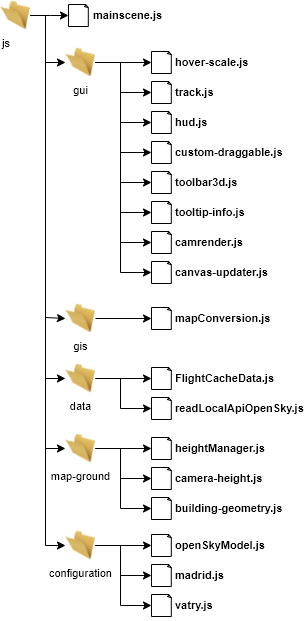
\includegraphics[width=6cm, keepaspectratio]{img/ficheros.drawio.png}
  \caption{Estructura de ficheros \textsc{JavaScript}.}
  \label{fig:javascriptFiles}
\end{figure}

\begin{center}
\begin{figure}[h]
  \centering
  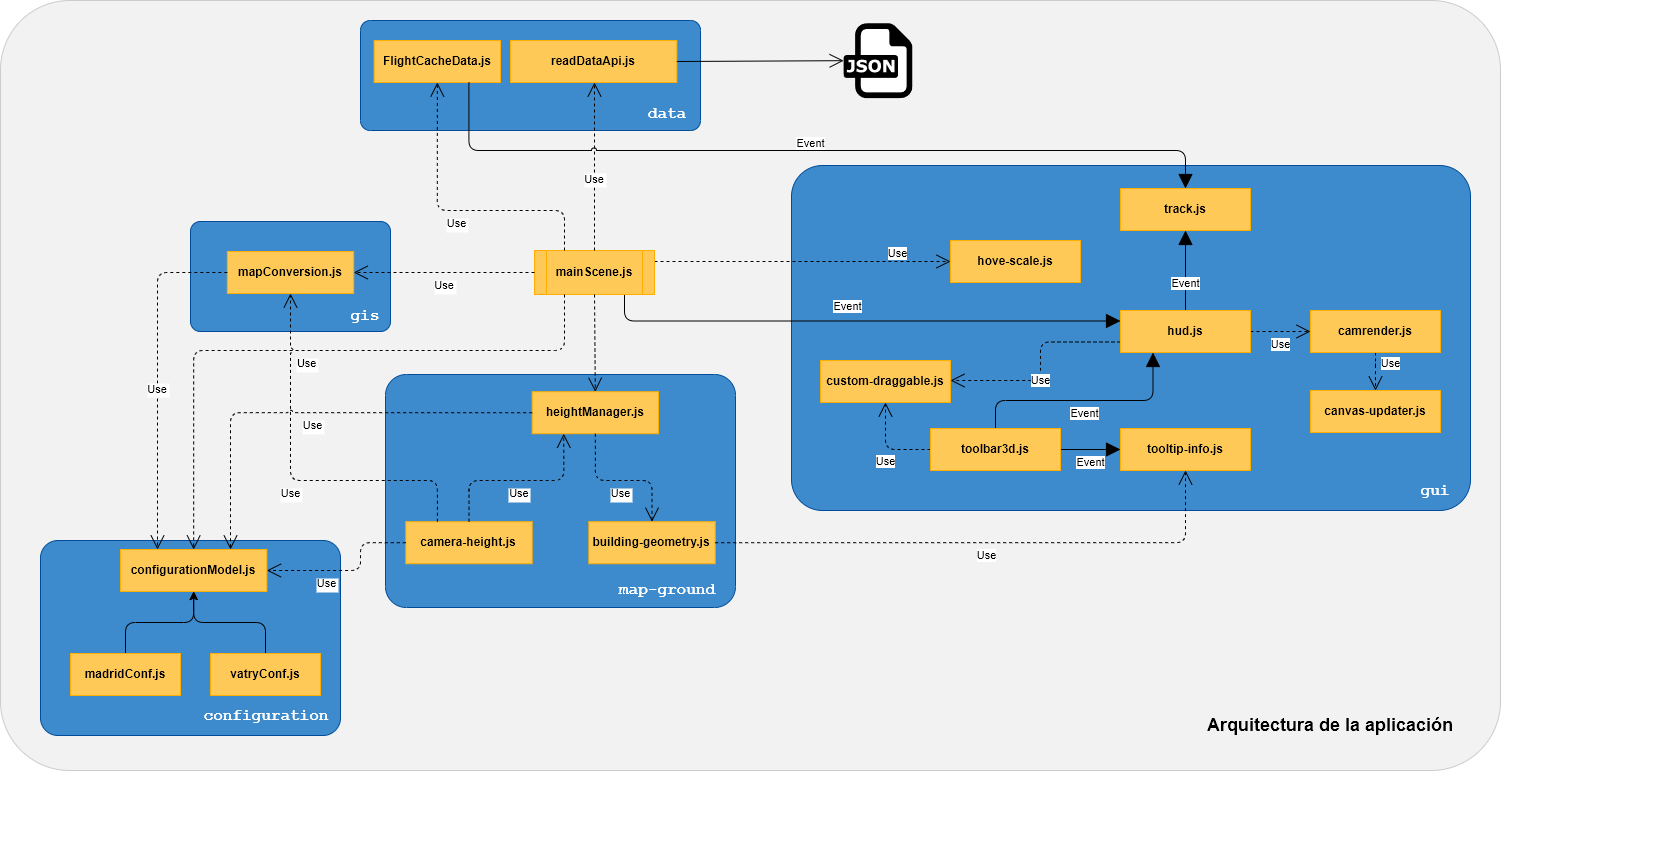
\includegraphics[width=18cm, keepaspectratio]{img/Arquitectura.png}
  \caption{Arquitectura general de la aplicación.}
  \label{fig:arquitectura}
\end{figure}
\end{center}
\section{Gestor de la escena principal}
\label{sec:mainScene.js}
El archivo \emph{mainSence.js} desempeña un papel fundamental en la aplicación, podemos describirlo como el núcleo central de la aplicación. Si nos referimos a la figura ~\ref{fig:arquitectura}, podemos apreciar su importancia. Su principal responsabilidad es sobrescribir el método de inicialización de la escena para agregar una función adicional que se invoca periódicamente según el intervalo de tiempo configurado.

El propósito de esta función adicional es obtener datos aeronáuticos de una \textsc{API}. Para lograr esto, se utiliza el archivo \emph{readLocalApiOpenSky.js}, que contiene la lógica para acceder a los datos en tiempo real o desde una caché local, dependiendo de la configuración establecida. Una vez que se obtienen los nuevos datos, se actualiza dinámicamente el escenario creando las entidades necesarias para representar la información aeronáutica en tiempo real.
En resumen, este archivo desempeña un papel central al proporcionar la funcionalidad esencial para la obtención y representación de datos aeronáuticos en el entorno \textsc{3D} de la aplicación.

\subsection{Componente main-scene}
\label{sec:mainScene}
Como mencionamos en la introducción, este archivo tiene la responsabilidad de sobrescribir las funciones \emph{init} y \emph{tick} del componente principal \emph{main-scene} en la escena de \textsc{A-Frame}. Esto permite agregar funcionalidades relacionadas con la obtención de datos de vuelo, la actualización de elementos en la escena y la interacción con las representaciones de aviones en el entorno \emph{\gls{3D}}.

En la función \emph{init}, utilizaremos la instancia única del convertidor de mapas de la clase \emph{MapConversion} que se encuentra en el archivo \emph{mapConversion.js}. Esto nos permitirá convertir la posición inicial de la cámara configurada a la posición que debe usar dentro del entorno \emph{3D}. Estableceremos las coordenadas \emph{X} y \emph{Z}, mientras que la altura se calculará posteriormente utilizando el componente \emph{heightManager} responsable de gestionar las alturas de la cámara a medida que se desplaza por el terreno.

Después, llamaremos a la instancia única del gestor de alturas \emph{HeightManager} para generar el suelo de la escena y los edificios correspondientes.
Finalmente, se establecerá una función que se invocará periódicamente según el intervalo de tiempo configurado para la actualización de los datos aeronáuticos. Es crucial que este intervalo de tiempo sea parametrizable, ya que representa el intervalo en el cual los datos pueden ser obtenidos cuando la consulta se realiza en modo \emph{online}. En el caso de utilizar una caché local, este intervalo de tiempo determinará la frecuencia con la que se han obtenido los datos, lo que permitirá que su representación se acerque lo más posible a la realidad. En caso de establecer un intervalo más corto al que se configuró al capturar los datos, estaremos representando la realidad de forma acelerada.

Es crucial comprender el concepto de una función con límite de frecuencia, también conocida como \emph{throttledFunction}, ya que no solo se utilizará en la actualización de datos aeronáuticos, sino que generalmente se empleará al implementar la función \emph{tick} de un componente. Este método se ejecuta automáticamente en cada cuadro renderizado por el motor de \emph{A-Frame}. Esto significa que el código dentro de la función \emph{tick} se ejecutará continuamente en cada repintado.
Es por eso que es importante tener en cuenta que el uso excesivo o ineficiente del método \emph{tick} puede afectar negativamente el rendimiento de la aplicación. 
Por lo tanto, la idea principal detrás de una \emph{throttledFunction} es limitar la cantidad de veces que una función puede ser llamada dentro de un período de tiempo determinado.
Al utilizar una \emph{throttledFunction} en la actualización de datos aeronáuticos, nos aseguramos de que la obtención y procesamiento de los datos se realice de manera controlada y eficiente. Esto evita llamadas excesivas a la \emph{\gls{API}} de datos y reduce la carga en el sistema, lo que mejora el rendimiento general de la aplicación en entornos \emph{3D}.
Después de comprender el concepto de la \emph{throttledFunction}, la última tarea que realiza el método de inicialización es establecer una función que utilizará esta técnica. Esta función se ejecutará periódicamente cada intervalo de tiempo configurado y utilizará el servicio \emph{readLocalApiOpenSky} para obtener los datos aeronáuticos.
Una vez que se obtengan los nuevos datos, la función invocará a \emph{updateData}, que está definida dentro del archivo \emph{mainScene.js}. En este punto, se realizará el análisis y parseo del archivo \emph{\gls{JSON}} que contiene los datos aeronáuticos. Si se encuentran nuevos componentes que deben ser creados en la escena, se generarán las entidades necesarias. Para los componentes existentes, se crearán animaciones que permitirán que los aviones se muevan de manera fluida dentro del entorno \emph{3D}.
Esta estrategia garantiza que los datos aeronáuticos se actualicen regularmente y que la representación de los aviones en la escena sea realista y dinámica.

Es importante remarcar que el componente \emph{main-scene} también será responsable de registrar los eventos necesarios para el envío de eventos sobre los elementos creados como aviones, para que el componente que explicaremos más adelante responsable de mostrar los datos reciba la información y el evento de mostrarse.

\subsection{Movimiento fluido de aviones dentro de la escena}
\label{subsec:movimientoFluido}
Para lograr un movimiento fluido de los aviones dentro de la escena, vamos a crear una interpolación lineal utilizando las animaciones proporcionadas por \textsc{A-Frame}, tal como se muestra en el código de la Figura \ref{codigo:movimientoFluido}. En esta implementación, cada vez que se ejecute el método de actualización de la escena en intervalos de tiempo regulares, crearemos una animación que interpolará de forma lineal la posición anterior y la nueva del avión. Esta animación tendrá una duración igual al intervalo de actualización asegurando de tal manera que la animación termina cuando ser recupera un nuevo dato para generar la siguiente.
\begin{figure}[h]
	\centering
	\begin{minted}[fontsize=\scriptsize, frame=single, numberblanklines=false]{javascript}
		if (cacheData.lastPosition != cacheData.newPosition) {
			entityEl.setAttribute('animation__000', {
				property: 'position',
				from: cacheData.lastPosition,
				to: cacheData.newPosition,
				autoplay: true,
				loop: 0,
				easing: 'linear',
				dur: intervalTime
			});
		}
	\end{minted}
	\caption{Animación para movimiento fluido interpolando posiciones de manera lineal.
		\label{codigo:movimientoFluido}}
\end{figure}

Para llevar a cabo esta tarea, es necesario mantener una caché de las entidades presentes en la escena y poder consultar rápidamente si existen y cuáles son sus datos antiguos. Además, esta caché nos será útil más adelante para implementar la funcionalidad que muestra el trayecto de un avión seleccionado en tiempo real, véase la sección \ref{subsec:track} para más información.

Dentro del archivo \emph{mainScene.js}, encontraremos una variable llamada \emph{flightsCache}, la cual es un mapa que contiene una instancia de la clase FlightCacheData~\ref{subsec:datosCacheVuelo} definida en el archivo \emph{FlightCacheData.js}, este mapa indexa el identificador del vuelo con su objeto caché para encontrar los datos de manera eficiente. Este mapa de objetos en caché será responsable de mantener el estado de los aviones en el mapa y nos permitirá consultar si un avión existe en la escena y cuál fue su posición anterior para la creación de la animación.
\begin{figure}[h]
	\centering
	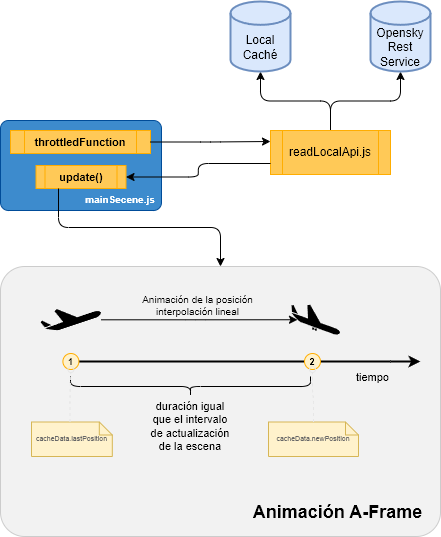
\includegraphics[width=12cm, keepaspectratio]{img/movimientoFluido.drawio.png}
	\caption{Animación A-Frame movimiento fluido.}
	\label{fig:movimientoFluido}
\end{figure}


\clearpage
\section{Gestión de la configuración de la aplicación}
\label{sec:configuration}
Debido a la naturaleza altamente reutilizable y configurable de nuestra aplicación, hemos dedicado especial atención a la parametrización de todos los componentes. Nuestro objetivo es que la creación de cualquier tipo de escenario se centre en un único archivo de configuración, simplificando así el proceso de establecer los parámetros necesarios para su correcto funcionamiento.

Para lograr esto, hemos desarrollado una pieza clave llamada \emph{configurationModel.js}, que contiene un módulo utilizado por todos los componentes de la aplicación. Este módulo almacena todos los parámetros específicos de un escenario en particular. Para establecer los valores internos de \emph{configurationModel.js}, creamos un archivo \textsc{JavaScript} que invoca los métodos \texttt{set} del módulo de configuración, estableciendo así todas las propiedades necesarias para el escenario tal y como podemos ver en la figura \ref{codigo:madridConf}. 
Como resultado, el archivo \textsc{HTML} principal de nuestro escenario carga el módulo de configuración y el archivo \textsc{JavaScript} que establece las propiedades requeridas para su correcto funcionamiento como se puede apreciar en la figura \ref{codigo:cargaConfiguracion}.
\begin{figure}[h]
\centering
\begin{minted}[fontsize=\scriptsize, frame=single, numberblanklines=false]{javascript}
    import * as configuration from "./configurationModel.js";
    //Establece las coordenadas geodésicas del escenario (latmin, latmax, longmin, longmax).
    configuration.setMerConfig(40.0234170,40.7441446,-4.2041338,-3.2538165);
    configuration.setCamPosition(40.50, -3.54);//posición de la cámara.
    configuration.setBuildingFileName('madrid_building');//carpeta de edificios.
    configuration.setFlightLocalFolder('_madrid');//carpeta caché de vuelos.
    configuration.setMapRaster('Madrid_raster.jpg');//fichero raster del terreno
    configuration.setMapDem('madrid_dem.bin');//fichero de alturas del terreno
    configuration.setLocalApiMode(true);//establece el modo offline datos cacheados.
    configuration.setDaoInterval(1000);//intervalo de refresco.
    configuration.setDaoLocalIndex(0);//indice del fichero por donde comienza.
    configuration.setApiUsuer('xxxx');//Establece el usuario para el modo online
    configuration.setApiPassword('xxxxx');//Establece la contraseña para el modo online
\end{minted}
\caption{Configuración del escenario de Madrid.
\label{codigo:madridConf}}
\end{figure}
\begin{figure}[h]
\centering
\begin{minted}[fontsize=\scriptsize, frame=single, numberblanklines=false]{html}
  <script src="js/configuration/configurationModel.js" type="module"></script>
  <script src="js/configuration/madridconf.js" type="module"></script>
\end{minted}
\caption{Carga del fichero del módulo gestor de configuración y el fichero que configura el escenario de Madrid.
\label{codigo:cargaConfiguracion}}
\end{figure}

\clearpage
\section{Sistema de información geográfica}
\label{sec:gis}
En esta sección, se describirá en detalle la implementación de toda la lógica de conversiones utilizada para georreferenciar las entidades dentro del escenario. También se abordarán los problemas que han surgido durante el proceso y las soluciones aplicadas, así como las librerías utilizadas.
\subsection{Gestor de conversiones del mapa}
\label{subsec:mapConversion}
En este fichero, se han implementado todas las funciones necesarias dentro de la aplicación para transformar coordenadas geoespaciales, en particular el objetivo principal de este gestor es la conversión de coordenadas expresadas en latitud y longitud en grados, a un vector válido para el escenario \gls{3D} (x, y, z).
Antes de adentrarnos en la descripción técnica, es importante hacer una breve introducción sobre los sistemas de referencia que vamos a utilizar y por qué es necesario realizar estas transformaciones.
En el mundo de los Sistemas de Información Geográfica (\textsc{\gls{gis}}), es común utilizar sistemas de referencia geoespaciales representados por coordenadas geográficas y sistemas de proyección cartográfica.
Una coordenada geográfica es un par de valores numéricos que representan la ubicación de un punto en la superficie de la Tierra. Como podemos observar en la figura \ref{fig:latlong} la \emph{latitud} y una \emph{longitud}, indican la posición definiendo la relación con los meridianos y paralelos terrestres.

\begin{figure}[h]
	\centering
	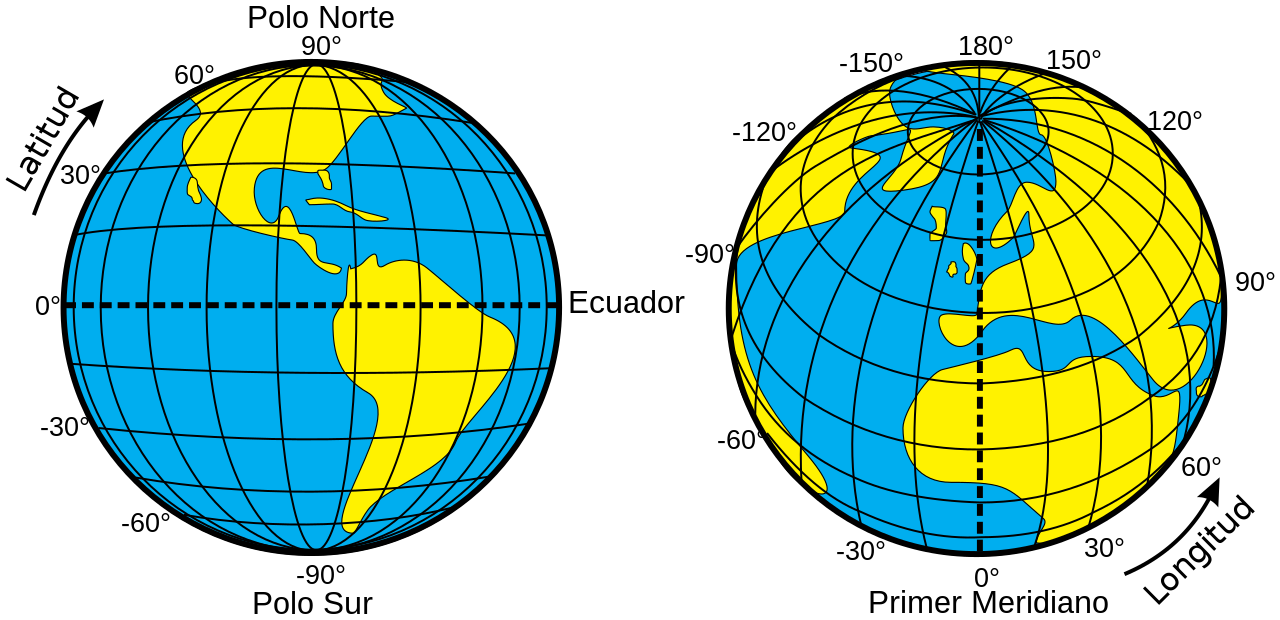
\includegraphics[width=12cm, keepaspectratio]{img/Latitud_y_Longitud_en_la_Tierra.svg.png}
	\caption{Coordenadas geográficas latitud y longitud.}
	\label{fig:latlong}
\end{figure}

En los sistemas de referencia geoespaciales, es común utilizar un datum que es un modelo matemático que describe la forma y la orientación de la Tierra, así como un punto de referencia. Muchos servicios y aplicaciones que proporcionan datos espaciales a nivel mundial, como \textsc{Google Maps} y \textsc{OpenSky}, utilizan el datum \textsc{WGS84} como su sistema de referencia estándar.
El datum \textsc{WGS84} (Sistema Mundial Geodésico de 1984) es ampliamente aceptado y utilizado en todo el mundo. Fue desarrollado por el Departamento de Defensa de los Estados Unidos y la Agencia Nacional de Inteligencia \gls{geoespacial} (\textsc{NGA}) como un sistema de referencia global para el intercambio de datos geoespaciales.
\textsc{WGS84} se basa en un modelo matemático que representa la forma de la Tierra como un elipsoide de revolución y establece un conjunto de parámetros para la conversión precisa entre coordenadas geográficas y sistemas de coordenadas proyectadas.
Dado que muchos servicios y datos geoespaciales se basan en \textsc{WGS84}, es importante que nuestra aplicación sea capaz de trabajar en este datum para garantizar la interoperabilidad y la correcta interpretación de los datos. Esto nos permite realizar conversiones precisas entre coordenadas geográficas en formato de \emph{latitud} y \emph{longitud}, y las coordenadas del escenario \textsc{3D} en el que estamos trabajando.
\begin{figure}[h]
	\centering
	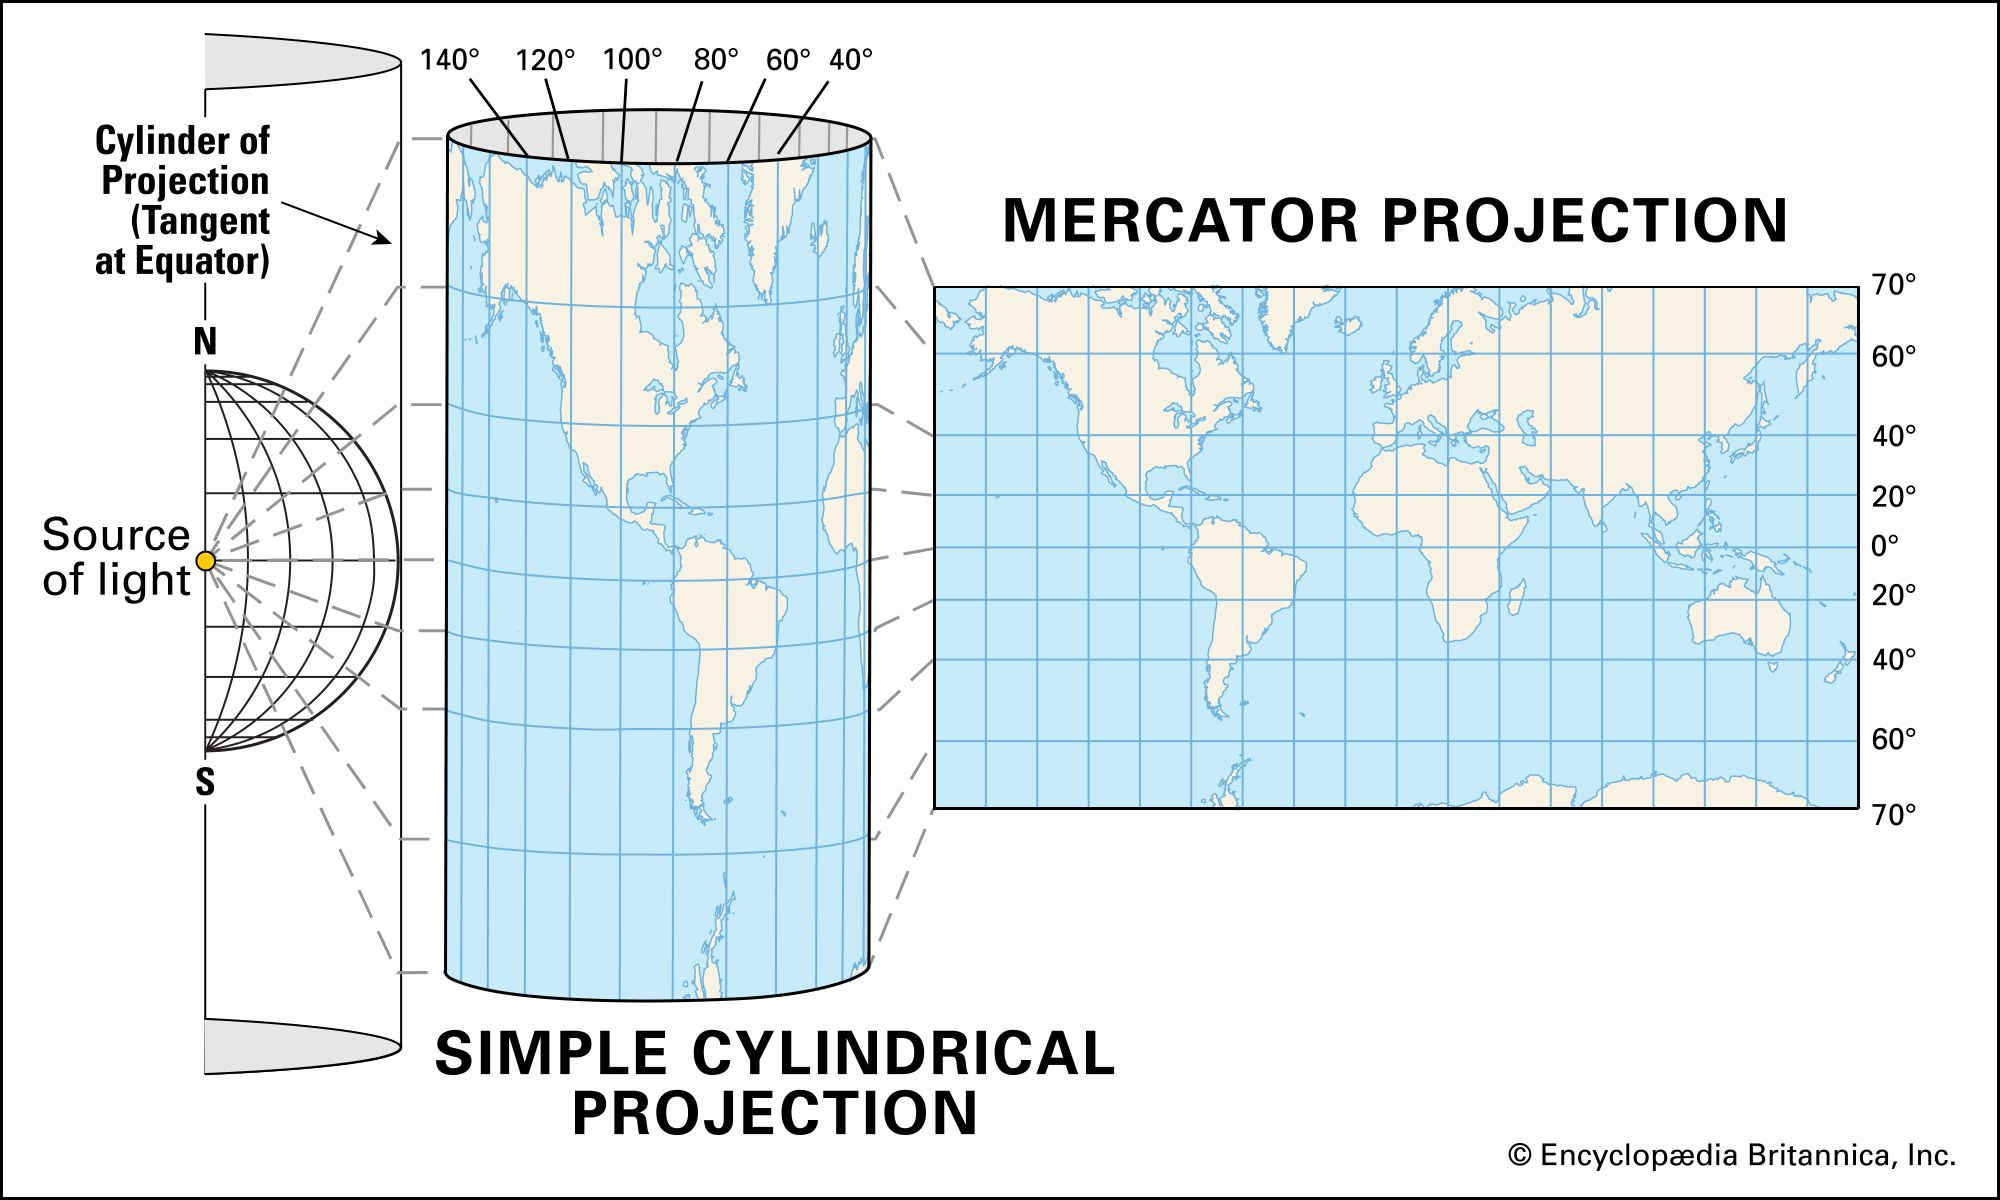
\includegraphics[width=12cm, keepaspectratio]{img/simple-cylindrical-projection-earth-map-globe-mercator.jpg}
	\caption{Proyección cilíndrica Mercator.}
	\label{fig:mercator}
\end{figure}
\\Por otro lado, un sistema de proyección cartográfica es una metodología que permite representar la forma curva de la Tierra en un plano. Debido a que nuestro planeta es un objeto tridimensional, es necesario utilizar proyecciones cartográficas para convertir la superficie esférica de la Tierra en un plano bidimensional. Estas proyecciones utilizan fórmulas matemáticas y parámetros específicos para lograr una representación precisa y adecuada de la Tierra en un mapa plano.
En nuestra aplicación, para convertir las coordenadas geoespaciales en un plano bidimensional, utilizaremos la proyección Mercator. Esta proyección es una de las proyecciones cartográficas más comunes y ampliamente utilizadas en internet. Fue desarrollada por Gerardus Mercator en el siglo XVI y se caracteriza por preservar los ángulos rectos y las formas de las áreas pequeñas, lo que la hace adecuada para representar regiones con menor extensión latitudinal. 
Se basa en envolver con un cilindro la superficie de la tierra y trazar una linea desde el centro terrestre hasta el plano del cilindro creando una relación entre el punto de intersección de la tierra con el del plano del cilindro tal y como podemos ver en la figura \ref{fig:mercator}.
\begin{figure}[H]
\begin{minipage}{0.7\textwidth}
Hablemos ahora del sistema de coordenadas de A-Frame, en el contexto del sistema de referencia 3D utilizado en A-Frame, se sigue la regla de la mano derecha. Esta regla establece la orientación de los ejes X, Y y Z en el espacio tridimensional.
Según la regla de la mano derecha, si extendemos el pulgar, el índice y el dedo medio de nuestra mano derecha de manera que sean perpendiculares entre sí, podemos asignar los ejes de la siguiente manera:
\begin{itemize}
    \item El pulgar representa el eje X, apuntando hacia la derecha.
    \item El índice representa el eje Y, apuntando hacia arriba.
    \item El dedo medio representa el eje Z, apuntando hacia adelante.
    
\end{itemize}
\end{minipage}
\hfill
\begin{minipage}{0.25\textwidth}
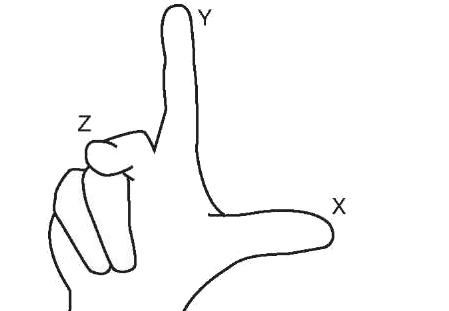
\includegraphics[width=\textwidth]{img/rightHand.jpg}
\caption{Regla de la mano derecha.}
\label{fig:rightHand}
\end{minipage}
\end{figure}
Esta convención es ampliamente utilizada en gráficos \textsc{3D} y programación, incluido el entorno de desarrollo \textsc{A-Frame}. Al seguir la regla de la mano derecha, podemos establecer una consistencia en la orientación de los ejes y facilitar la comprensión y manipulación de los objetos en el espacio tridimensional.
En este punto, nos enfrentamos al primer problema que debemos abordar en las conversiones. Si observamos una vista aérea tanto del suelo de nuestro escenario como de un mapa representado por un datum \textsc{WGS84} y proyectado con \textsc{Mercator}, notaremos una diferencia en las coordenadas.
La coordenada \textsc{Y}, que representa la latitud en el sistema \gls{geoespacial}, aumenta hacia arriba, mientras que en el sistema tridimensional, se representa a lo largo del eje \textsc{Z} y aumenta en dirección opuesta. Por lo tanto, esto es algo que debemos tener en cuenta al diseñar nuestras fórmulas de conversión.
Si observamos la figura \ref{fig:sistemasDeReferencia}, podemos apreciar cómo la posición con coordenada \texttt{(x=8, y=-7)} en el sistema \gls{geoespacial} se representa de manera diferente en ambos sistemas de referencia.
\begin{figure}[H]
  \centering
  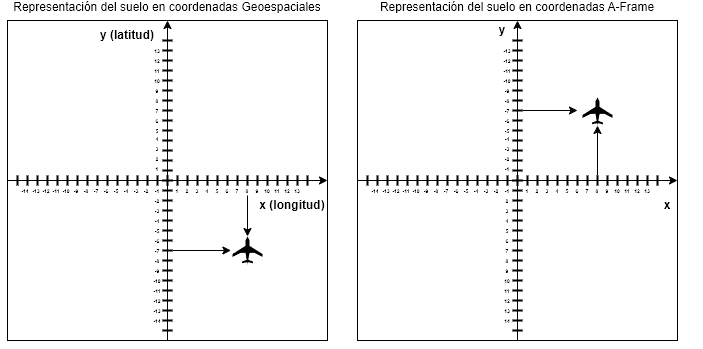
\includegraphics[width=13cm, keepaspectratio]{img/sistemasDeReferencia.drawio.png}
  \caption{Vista aerea de los sistemas de referencia.}
  \label{fig:sistemasDeReferencia}
\end{figure}

El siguiente problema al que nos enfrentamos está relacionado con las dimensiones de nuestra aplicación. Si consideramos cuidadosamente los escenarios que vamos a representar, el radio de alcance del escenario en kilómetros es considerablemente grande. \textsc{A-Frame} trabaja con unidades de metros, lo cual es adecuado para aplicaciones de realidad aumentada donde se busca que las dimensiones en el mundo 3D sean equivalentes a la realidad. Sin embargo, en el caso de nuestra aplicación, nuestro objetivo es asegurar que los aviones se puedan visualizar correctamente incluso a distancias de varios kilómetros. Manejar dimensiones tan grandes plantea problemas en el renderizado de objetos lejanos y en la interacción con entidades distantes, además de dificultades en el manejo de coordenadas 3D con unidades tan grandes.
Para ilustrar este concepto, consideremos el escenario de la demo de \emph{Vatry}, donde se configura un rectángulo con las siguientes coordenadas geoespaciales que representan \texttt{[xmin, xmax, ymin, ymax] = (48.491151723988, 49.027963936994, 3.7545776367187, 4.6238708496094)}. Utilizando un pequeño \emph{script} en \textsc{Google Earth Engine}, podemos calcular las distancias de altura y anchura para este rectángulo:
\begin{figure}[H]
	\centering
	\begin{minted}[fontsize=\scriptsize, frame=single, numberblanklines=false]{javascript}
		// Cargar el rectángulo de coordenadas geodésicas
		var rectangle = ee.Geometry.Rectangle(
		[3.7545776367187, 48.491151723988,4.6238708496094, 49.027963936994]);
		// Agregamos el rectángulo al mapa
		Map.addLayer(rectangle, {}, 'Rectángulo');
		// Centrar el mapa en el rectángulo
		Map.centerObject(rectangle, 10);
		// Obtener los límites del rectángulo
		var bounds = rectangle.bounds();
		var coordinates = bounds.coordinates().get(0);
		var firstCoordinate = ee.List(coordinates).get(0);
		var secondCoordinate = ee.List(coordinates).get(1);
		var thirdCoordinate = ee.List(coordinates).get(3);
		// creamos geometrías de tipo punto para calcular las distancias
		var punto1 = ee.Geometry.Point(firstCoordinate);
		var punto2 = ee.Geometry.Point(secondCoordinate);
		var punto3 = ee.Geometry.Point(thirdCoordinate);
		// Calcular la distancia
		var altura = punto1.distance(punto2).divide(1000);
		var anchura = punto1.distance(punto3).divide(1000);
		// Imprimir la altura y la anchura en la consola
		print('Altura del rectángulo:', altura);
		print('Anchura del rectángulo:', anchura);
	\end{minted}
	\caption{Cálculo de dimensiones para el escenario Vatry.
		\label{codigo:dimensionesVatry}
	}
\end{figure}
\begin{figure}[h]
	\centering
	\begin{minted}[fontsize=\scriptsize, frame=single, numberblanklines=false]{javascript}
	Altura del rectángulo:
	64.25269118063613
	Anchura del rectángulo:
	59.78757908704291
	\end{minted}
	\caption{Resultado del script.
	\label{codigo:resultadoDimensiones}
	}
\end{figure}
Como se puede observar en la figura \ref{codigo:resultadoDimensiones}, este \emph{script} nos arroja que estamos manejando distancias de aproximadamente 60 km. 
Por lo tanto, debemos tener en cuenta que cuando los aviones se alejan, se verán muy pequeños si representamos las unidades con una anchura de 60.000 unidades en el mundo 3D de A-Frame. Además, las operaciones como la intersección del rayo utilizado para seleccionar los aviones pueden presentar problemas y afectar el rendimiento de nuestra aplicación.
Para abordar esta situación, vamos a realizar una operación de escalado en nuestras ecuaciones. Esto nos permitirá dimensionar nuestro escenario de una manera más óptima, ajustando las unidades a una escala adecuada para asegurar una representación visual adecuada y un rendimiento eficiente.

El tercer problema al que nos enfrentamos es la asimetría en el escenario de representación. A menos que estemos representando una zona cercana al meridiano de \textsc{Greenwich} y al ecuador, al trabajar con coordenadas en metros es común que estemos manejando unidades excesivamente grandes. Por ejemplo, en la ciudad de \emph{Vatry}, las coordenadas se centran en aproximadamente x = 472476 e y = 6245020. A medida que nos alejamos, podemos encontrarnos con zonas de Rusia donde las coordenadas se expresan en millones de metros, lo cual hace que las operaciones resulten poco prácticas.
Para abordar este problema, se ha tomado la decisión de desplazar el centro del mapa al centro del escenario. Esto implica que, además del escalado mencionado anteriormente, realizaremos un desplazamiento de tal manera que el centro del escenario coincida con el centro del mapa.
Esta solución nos permite trabajar con dimensiones más manejables y evita la asimetría en la representación. Al centrar el mapa en el escenario, las operaciones y cálculos se realizan de manera más eficiente y se logra una representación equilibrada de los elementos geoespaciales en el entorno 3D.
Recapitulando, podemos resumir los siguientes puntos:
\begin{itemize}
    \item Nuestras transformaciones se centrarán en establecer las equivalencias de ejes entre los sistemas de referencia. En este caso, el eje \textsc{X} \gls{geoespacial} se mapeará al eje X en el mundo \textsc{3D}, el eje Y geoespacial se mapeará al eje \textsc{Z} en el mundo \textsc{3D}, y la altura se representará en el eje Y en el vector 3D.
    \item Habrá una inversión en el eje que representa la latitud. Esto significa que la coordenada Y geoespacial se mapeará al eje \textsc{-Z} en el mundo \textsc{3D} debido a la inversión.
    \item Se realizará un desplazamiento para centrar el escenario en la coordenada \texttt{(0,0,0)} en el mundo \textsc{3D}. Esto asegurará que el centro del escenario coincida con el origen de coordenadas en el mundo \textsc{3D}.
    \item Además, se aplicará un escalado para facilitar el dimensionado del escenario en el mundo \textsc{3D}. Esto permitirá trabajar con dimensiones más manejables y evitar problemas de representación y rendimiento.
\end{itemize}
En resumen, estas transformaciones nos permitirán establecer una correspondencia adecuada entre los sistemas de referencia geoespacial y el entorno 3D, asegurando una representación coherente y optimizada de los elementos geoespaciales en nuestro escenario.

Para la conversión de coordenadas de \textsc{WGS84} en grados a metros, hemos optado por utilizar la librería \textsc{Leaflet}~\ref{sec:leaflet} en lugar de las fórmulas clásicas de la proyección \textsc{Mercator}. Las razones principales que respaldan esta elección son las siguientes:
\begin{itemize}
    \item \textbf{\emph{Facilidad de uso}}: \textsc{Leaflet} proporciona una interfaz intuitiva y sencilla para trabajar con diversos sistemas de coordenadas y proyecciones. La librería admite múltiples sistemas de proyección, incluyendo la proyección \textsc{Mercator} ampliamente utilizada. 
    Además, ofrece funciones integradas para realizar conversiones de coordenadas y proyecciones, lo cual simplifica la transformación de datos geoespaciales en el contexto del mapa.
    \item \textbf{\emph{Optimización de rendimiento}}: \textsc{Leaflet} está diseñado para ofrecer un rendimiento óptimo en entornos web en tiempo real. Sus conversiones están optimizadas para asegurar un alto rendimiento.
    \item \textbf{\emph{Mantenibilidad y actualizaciones regulares}}: \textsc{Leaflet} cuenta con una comunidad activa de desarrolladores que constantemente trabajan en mejorar la biblioteca, solucionar problemas, agregar nuevas características y garantizar la compatibilidad con las últimas tecnologías y estándares. Esto brinda confianza en la estabilidad y continuidad del proyecto, al tiempo que reduce la carga de mantenimiento para nuestro prototipo.
\end{itemize}
A continuación, en la Figura \ref{formula:desplazamiento}, se presenta el cálculo del desplazamiento. Se puede observar que primero se calculan las coordenadas geodésicas del centro del escenario. Para ello, se toma el punto medio de la latitud y la longitud. Dado que deseamos desplazar el centro del escenario al punto \emph{(0,0,0)} en el mundo \textsc{3D}, es necesario tener previamente calculado el desplazamiento en metros que se aplicará a cada coordenada.

Posteriormente, se utiliza una función que realiza la conversión a metros mediante la proyección de \textsc{Mercator} \ref{funcion:deegreeToMeter}. Esto da como resultado las coordenadas cartesianas del centro del escenario expresadas en metros. Estas coordenadas representan el desplazamiento que se aplicará a cada coordenada para lograr que el mapa esté centrado en el punto \emph{(0,0,0)}.
\begin{figure}[h]
\begin{align*}
\text{\emph{long}} &= \frac{{\text{LONG\_MIN} + \text{LONG\_MAX}}}{2} \\
\text{\emph{lat}} &= \frac{{\text{LAT\_MIN} + \text{LAT\_MAX}}}{2} \\
\text{\emph{displacement}} &= \texttt{\text{degreeToMeter}(\text{lat}, \text{long})}
\end{align*}
\caption{Calculo del desplazamiento del escenario.}
  \label{formula:desplazamiento}
\end{figure}

Por lo tanto, el constructor de nuestra clase \emph{MapConversion} realizará estos cálculos y almacenará el resultado en una \emph{instancia única} para que pueda ser utilizado en todas las funciones de conversión. De esta manera, evitamos repetir los cálculos y garantizamos que todas las transformaciones se realicen utilizando el mismo desplazamiento y escala.
\subsubsection{De WGS84 a Mercator}
\label{funcion:deegreeToMeter}
Esta función utiliza la librería \textsc{Leaflet} para crear una coordenada geodésicas en el sistema de referencia \textsc{WGS84} a partir de una \emph{latitud} y \emph{longitud} dadas. Luego, realiza la proyección en \textsc{Mercator} para convertir la coordenada geodésica en una coordenada cartesiana expresada en metros.
\subsubsection{De Mercator a WGS84}
\label{funcion:meterToDegree}
Esta función realiza la operación inversa a la función descrita en \ref{funcion:deegreeToMeter}. Convierte una coordenada cartesiana en el sistema de proyección \textsc{Mercator} a una coordenada geodésica en el sistema de referencia \textsc{WGS84} haciendo uso de la librería \textsc{Leaflet}. Esta función aprovecha sus capacidades integradas para realizar la desproyección de coordenadas.
\subsubsection{De MatorToWorld}
Esta función se encargará de realizar la conversión de una coordenada cartesiana en proyección \textsc{Mercator} a una coordenada en el mundo 3D. Su objetivo principal es aplicar las transformaciones mencionadas anteriormente para abordar los problemas de representación, que incluyen la inversión del eje \textsc{Z}, el desplazamiento y el escalado. Para lograr esto, la función hará uso del desplazamiento calculado en el constructor de la clase. A continuación, se presentan las fórmulas que serán aplicadas:

\begin{figure}[h]
    \begin{align*}
    X_{\text{3DWorld}} &= \frac{\mathbf{\mathrm{mercatorVector}}_{\text{x}} - \mathbf{\mathrm{displacement}}_{\text{x}}}{\mathbf{\mathrm{FACTOR}}} \\
    Y_{\text{3DWorld}} &= \frac{\mathbf{\mathrm{mercatorVector}}_{\text{z}} - \mathbf{\mathrm{displacement}}_{\text{y}}}{\mathbf{\mathrm{FACTOR}}} \\\\
    \mathbf{\mathrm{3DWorld}} &= 
    \begin{bmatrix}
    X_{\text{3DWorld}}, \frac{\mathrm{height}}{\mathbf{\mathrm{FACTOR}}}, -Y_{\text{3DWorld}}
    \end{bmatrix}
    \end{align*}
\caption{Calculo de la conversión de coordenadas cartesianas en \textsc{Mercator} a mundo \textsc{3D}.}
  \label{formula:mercatorToWorld}
\end{figure}

\subsubsection{De mundo 3D a Mercator}
\label{funcion:worldtoMercator}
Esta función tiene la responsabilidad de realizar la operación inversa a la función mencionada en \ref{funcion:mercatorToWorld}. Su objetivo es convertir un vector del escenario 3D en una coordenada cartesiana en proyección \textsc{Mercator}, aplicando todas las operaciones inversas al escalado, la inversión de ejes y el desplazamiento realizados por la función \emph{Mercator a mundo 3D}~\ref{funcion:mercatorToWorld}. A continuación, se presentan las fórmulas que serán aplicadas:

\begin{figure}[h]
\begin{align*}
X_{\text{Mercator}} &= (\mathbf{\mathrm{world3DVector}}_{\text{x}} \times \mathbf{\mathrm{FACTOR}}) + \mathbf{\mathrm{displacement}}_{\text{x}} \\
Y_{\text{Mercator}} &= (\mathbf{\mathrm{world3DVector}}_{\text{z}} \times \mathbf{\mathrm{FACTOR}}) + \mathbf{\mathrm{displacement}}_{\text{y}} \\
\mathbf{\mathrm{Mercator}} &= 
\begin{bmatrix}
X_{\text{Mercator}}, \mathbf{\mathrm{world3DVector}}_{\text{y}} \times \mathbf{\mathrm{FACTOR}}, -Y_{\text{Mercator}}
\end{bmatrix}
\end{align*}
\caption{Calculo de la conversión vector 3D a coordenadas cartesianas Mercator.}
  \label{formula:worldtoMercator}
\end{figure}

\subsubsection{De WGS84 a mundo 3D}
\label{funcion:degreeToWorld}
Esta función se basará en la función \emph{de WGS84 a Mercator} \ref{funcion:deegreeToMeter} para convertir las coordenadas de \emph{latitud} y \emph{longitud} en formato \textsc{WGS84} a una proyección \textsc{Mercator}. A continuación, utilizará la función \emph{Mercator a mundo 3D}~\ref{funcion:mercatorToWorld} para transformar la coordenada \textsc{Mercator} resultante en una coordenada tridimensional en el mundo \textsc{3D}. En resumen, esta función permitirá convertir una coordenada geodésica en una coordenada \textsc{3D} sin altura, lo que facilitará la ubicación de las entidades del mundo real dentro del escenario.

Esta función será útil para posicionar entidades geoespaciales, como edificios o aviones, dentro del escenario. Además, en un futuro, podría utilizarse para crear cualquier tipo de entidad que se base en datos geodésicos, ya que la amplia mayoría de servicios utiliza el sistema \textsc{WGS84} y está función nos devuelve el vector de posición para el escenario \textsc{A-Frame}.

\subsubsection{De mundo 3D a WGS84}
\label{funcion:worldToDegree}
Esta función se encargará de realizar la operación inversa a la función \emph{WGS84 a mundo 3D} descrita en la sección \ref{funcion:degreeToWorld}. Su objetivo es obtener la coordenada geodésica a partir de un vector tridimensional del mundo 3D. Para lograr esto, primero se realizará la conversión de la coordenada \textsc{3D} a una coordenada \textsc{Mercator} utilizando la función \emph{mundo 3D a Mercator} mencionada en la sección \ref{funcion:worldtoMercator}. Luego, se aplicará la conversión de la coordenada cartesiana a \textsc{WGS84} utilizando la función \emph{de Mercator a WGS84} descrita en la sección \ref{funcion:meterToDegree}.

Aunque esta función no se utiliza actualmente en la aplicación, resulta útil para futuras funcionalidades. Por ejemplo, podría emplearse para mostrar la ubicación de la cámara principal en el \textsc{\gls{HUD}}, proporcionando las coordenadas geodésicas correspondientes a la posición de la entidad de la cámara. Su implementación sería sencilla gracias al uso de esta función para convertir el vector de posición en el mundo 3D en una coordenada geodésica en formato \textsc{WGS84}.

\subsubsection{Devuelve el tamaño del terreno}
\label{funcion:getGroundSize}
La función proporcionará las dimensiones del escenario en el entorno \textsc{3D} al utilizar las constantes que definen la \emph{latitud} y \emph{longitud} máxima del rectángulo del escenario geodésico. Mediante la transformación de estas coordenadas al sistema de coordenadas del mundo \textsc{3D} y considerando que el escenario está centrado, podremos calcular con precisión las dimensiones de anchura y altura en el entorno tridimensional (Mundo 3D). Esta función será de gran utilidad en etapas posteriores para el gestor del terreno del escenario, ya que se requieren estas dimensiones para el correcto funcionamiento del componente de terreno descrito en la sección \ref{subsec:heightManager}.

\subsubsection{Crear entidades en los corner del terreno}
\label{funcion:createCorner}
Esta función no tiene ninguna aplicación en el prototipo final, su único propósito es facilitar la depuración y verificar el correcto funcionamiento de las transformaciones de esta clase. Crea entidades en las esquinas del escenario y proporciona una referencia visual del terreno en el escenario para comprobar si está correctamente centrado en el entorno tridimensional, son funciones necesarias que se han creado para una depuración visual en el inspector del escenario.
\clearpage
\section{Terreno en el mapa}
\label{sec:mapGround}
En esta carpeta se encuentran todos los archivos responsables de gestionar la lógica relacionada con el suelo y las entidades asociadas. El objetivo de estos archivos es gestionar todas las operaciones relacionadas con el suelo, desde la generación del mallado hasta el posicionamiento y desplazamiento de las entidades sobre la superficie del suelo. Para lograr esto, se utilizan diversas tecnologías y librerías que permiten realizar las operaciones necesarias de forma eficiente y precisa.
También podremos encontrar las entidades que serán colocadas sobre el suelo, como la cámara principal que se moverá sobre la superficie del terreno y los edificios que deben estar alineados con el suelo. Para modelar las superficies, se utilizan conjuntos de datos \gls{raster}. Un raster es una matriz compuesta por celdas o píxeles dispuestos en filas y columnas que cubren una determinada región geográfica.
Cada celda en la matriz representa una unidad de área cuadrada y contiene un valor numérico que representa una altura tal y como podemos apreciar en la figura \ref{fig:dem}.

Un archivo DEM es un tipo de archivo raster con celdas que representan un valor de elevación correspondiente a una ubicación geodésica específica en relación a un datum de referencia. En resumen, un archivo DEM es una representación muestreada de una superficie terrestre limitada, donde las alturas se almacenan en una matriz.

\begin{figure}[h]
  \centering
  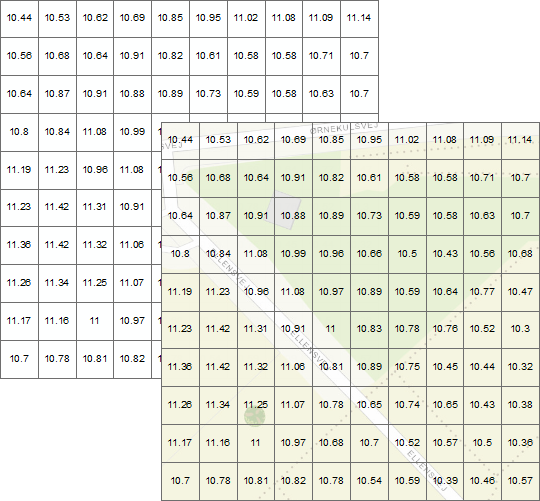
\includegraphics[width=8cm, keepaspectratio]{img/dem.png}
  \caption{Representación del contenido de un fichero DEM.}
  \label{fig:dem}
\end{figure}

Para crear la entidad del terreno, este componente requiere varios parámetros. En primer lugar, se necesita un archivo DEM que contenga la información de elevación del terreno. Además, se deben proporcionar los siguientes argumentos:
\begin{itemize}
	\item las dimensiones de la entidad en el escenario para lo cual se creó la función descrita en la sección \ref{funcion:getGroundSize}.
	\item la textura que se utilizará para pintar el terreno.
	\item la resolución del terreno (dimensiones de la matriz de alturas).
	\item un parámetro de magnificación de alturas que controla la escala de las elevaciones del terreno en relación con la entidad visual resultante, de esto hablaremos más adelante pero este parámetro define el valor máximo en el mundo 3D para la altura más alta del fichero de alturas, esto es debido a que se normalizan los valores.
\end{itemize}
Con estos parámetros, el componente \emph{aframe-terrain-model-component} genera y renderiza el terreno en el escenario, permitiendo así la representación realista de la superficie terrestre.
\subsection{Generación del fichero DEM}
\label{sec:dem}
En primer lugar, vamos a detallar el proceso utilizado para generar el archivo de alturas \textsc{DEM} en formato \textsc{ENVI}, que luego se inyectará en el componente \emph{aframe-terrain-model-component}.
Basándonos en la experiencia del tutor del proyecto, el \emph{Dr. Jesús M. González Barahona}, quien ha investigado y experimentado con la carga de terrenos del programa \textsc{Copernicus} de la Unión Europea a través transformaciones con las herramientas proporcionadas por \textsc{GDAL}, una biblioteca de código abierto ampliamente utilizada en el campo de los sistemas de información geográfica que permite la manipulación de datos geoespaciales.
Vamos a describir los pasos para generar el fichero \textsc{DEM} de Madrid como ejemplo:
\label{manual:generacionDem}
\begin{enumerate}
    \item Primero, procedemos a descargar la zona de interés de los servidores de \textsc{Copernicus}, que contiene el área correspondiente a las coordenadas donde generaremos el archivo \textsc{DEM}. Para realizar esto, visitamos la página \url{https://land.copernicus.eu/imagery-in-situ/eu-dem/eu-dem-v1.1} y observamos en la Figura \ref{fig:copernicus} los cuadrantes relevantes para extraer el archivo \textsc{DEM} de Madrid, que son \textsc{E30N10} (30º Este 10º Norte) y \textsc{E30N20} (30º Este 20º Norte). Por lo tanto, procedemos a descargar los binarios correspondientes a estas áreas.
\begin{figure}[h]
  \centering
  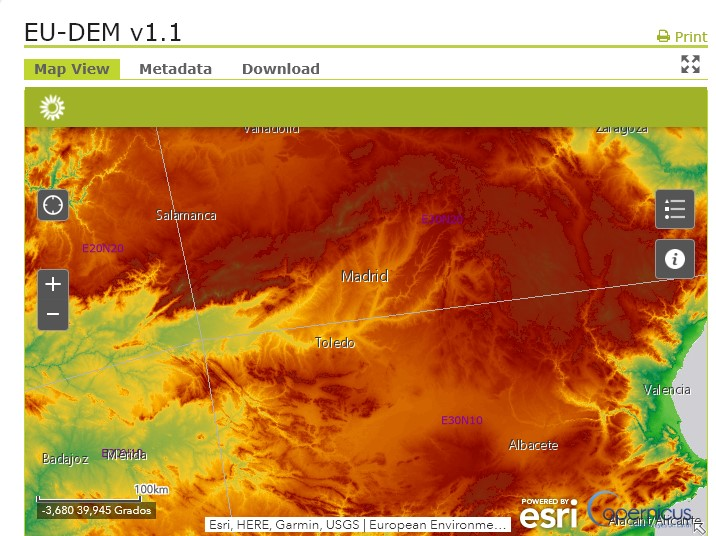
\includegraphics[width=8cm, keepaspectratio]{img/copernicus.jpg}
  \caption{Visor online de ficheros DEM Copernicus.}
  \label{fig:copernicus}
\end{figure}
    \item Utilizamos el comando \texttt{gdalbuildvrt} para crear un archivo \textsc{VRT} llamado \emph{map.vrt} que contiene un mosaico virtual de los archivos \gls{raster} \url{eu_dem_v11_E30N10.TIF} y \url{eu_dem_v11_E30N20.TIF}. Esto permite acceder y trabajar con los datos de elevación contenidos en ambos archivos como si fueran un solo conjunto de datos, sin necesidad de fusionar físicamente los archivos originales. El archivo \textsc{VRT} proporciona una vista virtual de los datos raster y permite un acceso eficiente y flexible a los mismos.

    {\scriptsize
    \begin{verbatim}
    gdalbuildvrt map.vrt eu_dem_v11_E30N10.TIF eu_dem_v11_E30N20.TIF
    \end{verbatim}
    }
    
    \item Los ficheros que hemos descargado están proyectados en el sistema de referencia EPSG:3035\footnote{\url{https://epsg.io/3035}}, que utiliza la proyección \textsc{UTM} (Universal Transverse \textsc{Mercator}). Para realizar la transformación, utilizamos el comando \texttt{gdalwarp} que toma un archivo \textsc{VRT} llamado \emph{map.vrt} y lo convierte en un nuevo archivo \textsc{TIFF} llamado \emph{smallMap.tif}. Durante este proceso, los datos se reproyectan al sistema de referencia espacial \textsc{EPSG:4326}\footnote{\url{https://epsg.io/4326}}, que utiliza el \textsc{DATUM WGS84} y es el sistema de referencia que utilizamos para los datos de las \gls{API}. Luego, los datos se recortan para abarcar la extensión definida por los límites de \emph{latitud} y \emph{longitud} proporcionados al comando.

    {\scriptsize
    \begin{verbatim}
    gdalwarp -t_srs EPSG:4326 -te -4.204133836988655 40.023417003380956
    -3.253816454176155 40.744144594569384 map.vrt smallMap.tif
    \end{verbatim}
    }

    \item Comprobamos las coordenadas del fichero resultante.

    {\scriptsize
    \begin{verbatim}
    gdalinfo -mm smallMap.tif

    Corner Coordinates:
    Upper Left  (  -4.2041338,  40.7441446) (  4d12'14.88"W, 40d44'38.92"N)
    Lower Left  (  -4.2041338,  40.0234170) (  4d12'14.88"W, 40d 1'24.30"N)
    Upper Right (  -3.2538165,  40.7441446) (  3d15'13.74"W, 40d44'38.92"N)
    Lower Right (  -3.2538165,  40.0234170) (  3d15'13.74"W, 40d 1'24.30"N)
    Center      (  -3.7289751,  40.3837808) (  3d43'44.31"W, 40d23' 1.61"N)
    Band 1 Block=3671x1 Type=Float32, ColorInterp=Gray
        Computed Min/Max=461.652,1886.917
      NoData Value=-3.4028234663852886e+38
    \end{verbatim}
    }
    \item Podemos utilizar el comando \texttt{gdal translate} para generar un archivo \textsc{PNG} que nos permita visualizar los datos generados a partir del archivo de alturas. Esto nos brindará una representación en blanco y negro de la superficie como se puede observar en la figura \ref{fig:demImage}.
    {\scriptsize
    \begin{verbatim}
    gdal_translate -scale 0 2522 0 255 -outsize 200 200 -of PNG smallMap.tif smallMap.png
    \end{verbatim}
    }
    
    \begin{figure}[h]
      \centering
      
\includegraphics[width=8cm, keepaspectratio]{img/smallMap.png}
      \caption{Fichero de alturas smallMap.png visto como imagen en blanco y negro.}
      \label{fig:demImage}
    \end{figure}

    \item A continuación, haremos uso de nuevo del comando \texttt{gdal translate} para realizar un escalado de valores. Transformaremos el rango original de \emph{(0,2522)} a un nuevo rango de \emph{(0,65535)}, que corresponde al rango del tipo de datos \texttt{UInt16} que usa el componente para almacenar los datos. El resultado será guardado en un archivo binario \textsc{ENVI} llamado \emph{Madrid.bin}.

    {\scriptsize
    \begin{verbatim}
    gdal_translate -scale 0 2522 0 65535 -ot UInt16 -outsize 200 200 -of ENVI smallMap.tif Madrid.bin
    \end{verbatim}
    }
\end{enumerate}

\subsection{Generación de la capa de textura raster}
\label{sec:raster}
Vamos a describir cómo utilizando la tecnología que nos brinda \textsc{Google Earth Engine} podemos extraer la capa \gls{raster} correspondiente a las coordenadas del rectángulo para el cual hemos generado el archivo bin en formato \textsc{ENVI}. Esto nos permitirá superponer la textura del terreno con una imagen satelital que esté georreferenciada con las mismas coordenadas, lo que nos dará una representación más realista del terreno.
En la figura \ref{codigo:generacionRasterMadrid} se puede observar que estamos usando el \textsc{API} que ofrece el \gls{framework} de \textsc{Google Earth Engine}, el objeto \texttt{ee} (Earth Engine) nos ofrece la capacidad de crear geometrias añadirlas al mapa y realizar operaciones con ellas, a continuación paso a describir el proceso que seguimos para realizar la extracción del raster:
\begin{enumerate}
    \item Creamos una geometría rectangular con coordenadas \textsc{WGS84} que nos permitirá realizar una operación de intersección con el raster para la obtención de una porción.
    \item Añadimos el rectángulo como capa para visualizar la zona que vamos a exportar y realizar una comprobación visual de los datos.
    \item Cargamos una colección de imágenes satelitales Sentinel-2, filtrando por las capturadas entre el 1 de enero de 2019 y el 28 de febrero de 2019.
    \item Creamos un mosaico de las imágenes de la colección. Esto combina todas las imágenes en una sola imagen, seleccionando los píxeles en función de su importancia o calidad. Añadimos este mosaico como capa para visualizar el resultado.
    \item Creamos una imagen \textsc{RGB} utilizando las bandas B4, B3 y B2.
    \item Exportamos la imagen \textsc{RGB} en formato \textsc{GeoTIFF}, utilizando una escala de 20 metros por píxel y el sistema de coordenadas \textsc{EPSG:3857}. Utilizamos \textsc{EPSG:3857} porque utiliza el \textsc{Datum WGS84} y proyecta en \textsc{Mercator}, que es el sistema de coordenadas comúnmente utilizado por \textsc{Google Maps} y \textsc{OpenStreetMaps}. De esta manera, obtenemos el raster proyectado en \textsc{Mercator} directamente, que es lo que necesitamos.
    En la figura \ref{fig:dem}, se muestra el resultado de la exportación. Mientras que en la figura \ref{fig:demAframe}, se presenta una escena simple en A-Frame donde visualizamos el raster exportado sobre una malla con las alturas obtenidas del fichero DEM de Madrid. En esta representación, se pueden apreciar claramente las montañas y las alturas alrededor del aeropuerto de Madrid.
\end{enumerate}
\label{manual:generacionRaster}
\begin{figure}[H]
\centering
\begin{minted}[fontsize=\scriptsize, frame=single, numberblanklines=false,breaklines]{javascript}
var geometry = ee.Geometry.Rectangle(-4.204133836988655,40.023417003380956, -3.253816454176155,40.744144594569384);
 // Convierte la geometría a un objeto Feature y establece un nombre
var rectangulo = ee.Feature(geometry, {nombre: 'Mi rectángulo'});
// Añade el rectángulo a la vista del Mapa
Map.addLayer(rectangulo, {}, 'Rectángulo');
var ColeccionSentinel = ee.ImageCollection('COPERNICUS/S2').filterDate('2019-01-01', '2019-02-28');
var Mosaico = ColeccionSentinel.mosaic();
Map.addLayer(Mosaico, {max: 5000.0,min: 0.0,gamma: 1.0,bands: ['B4', 'B3', 'B2']},
    'Composicion RGB');
// Crear una imagen RGB utilizando las bandas B4, B3 y B2
var RGB = Mosaico.visualize({bands: ['B4', 'B3', 'B2'], max: 5000, min: 0, gamma: 1.0});
// Crea un objeto Projection a partir de la identificación EPSG
var epsg3857 = 'EPSG:3857';
// Descargar la imagen RGB en formato GeoTIFF
Export.image.toDrive({image: RGB,description: 'Sentinel2_RGB',scale: 20,crs:epsg3857, region: geometry, maxPixels: 28710052848});
\end{minted}
\caption{Código Javascript para la generación de la capa raster de textura de Madrid.
\label{codigo:generacionRasterMadrid}
}
\end{figure}

\begin{figure}[h]
  \centering
  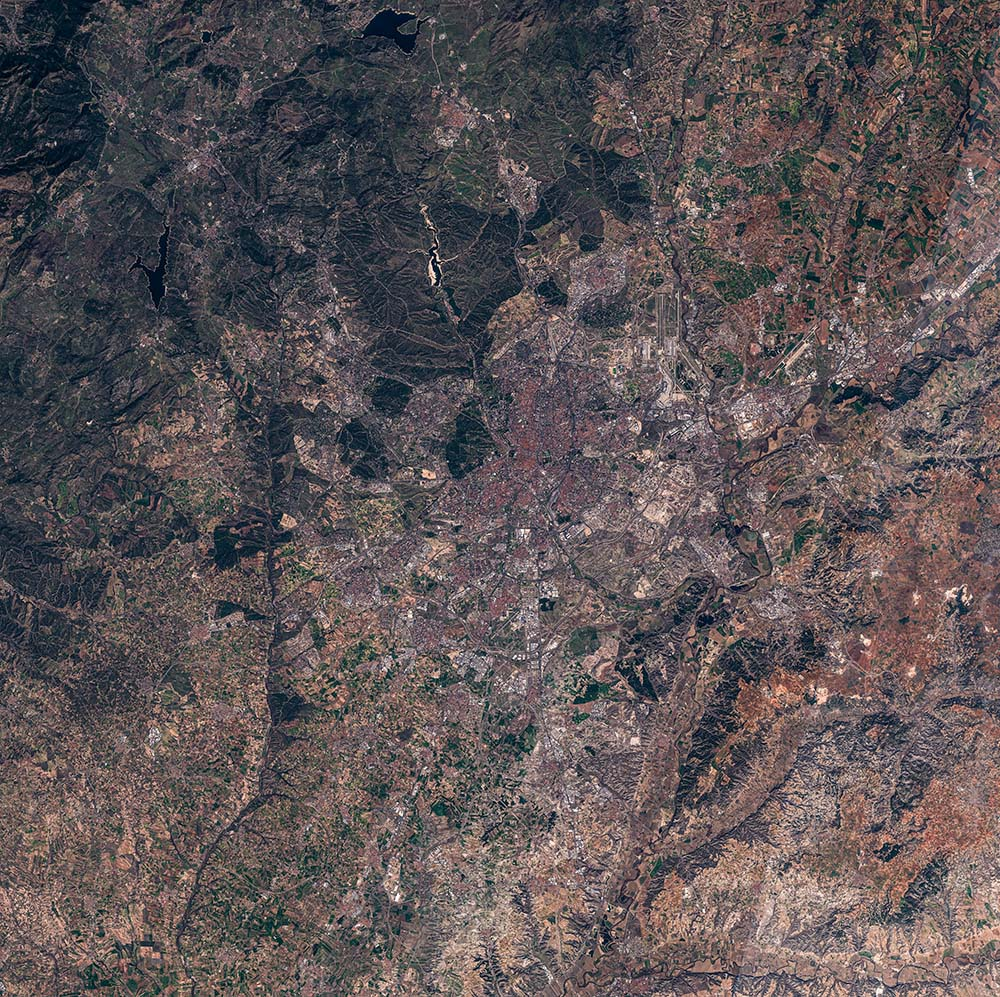
\includegraphics[width=8cm, keepaspectratio]{img/Madrid_raster.jpg}
  \caption{Raster de Madrid generado con Google Earth Engine.}
  \label{fig:demMadrid}
\end{figure}

\begin{figure}[h]
  \centering
  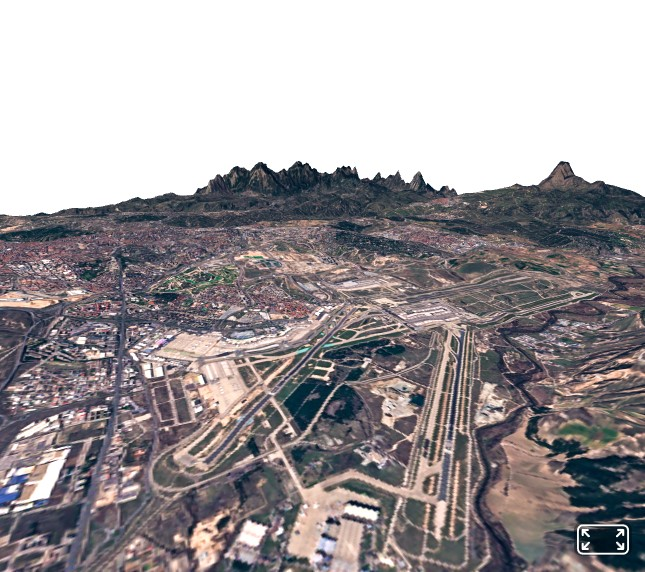
\includegraphics[width=8cm, keepaspectratio]{img/madrid_terrain.jpg}
  \caption{Resultado final del componente con la textura de Madrid y el fichero DEM generado.}
  \label{fig:demAframe}
\end{figure}

\subsection{Gestor de alturas}
\label{subsec:heightManager}
El gestor de alturas es una clase en \textsc{JavaScript} encargada de administrar el terreno en el escenario. En nuestra aplicación, utilizaremos una única instancia de este gestor para aprovechar el almacenamiento de los datos de las alturas durante la carga del terreno. Además, el gestor proporcionará funcionalidades para obtener las alturas de puntos específicos en el escenario \textsc{3D}. En la inicialización del escenario principal descrita en la sección \ref{sec:mainScene.js}, el gestor de la escena invocará los métodos para cargar el terreno y los edificios.
Un problema común al reutilizar componentes de \textsc{A-Frame} creados por otros desarrolladores, como en este caso el componente utilizado para generar el mallado del terreno con \textsc{Three.js}, es la dificultad para acceder a los datos leídos del archivo binario que contiene las alturas. Esta falta de documentación y de una \gls{API} específica para acceder a los datos puede ser un obstáculo.
Sin embargo, al analizar la implementación del componente \emph{aframe-terrain-model-component}, descubrimos que después de leer el archivo se emite un evento que contiene el objeto con los datos de alturas.
Aprovechando esta información, nos suscribimos al evento una vez que creamos el componente del terreno. De esta manera, podemos recibir y almacenar la matriz de alturas preparando nuestra instancia única para atender peticiones que requieran la altura para un punto del mundo 3D.

Es importante tener en cuenta que otros componentes, como el gestor de altura de la cámara o las geometrías de los edificios, necesitarán acceder a la altura en puntos específicos del escenario y podrán hacerlo a través de la \textsc{API} proporcionada por la instancia única de esta clase.
\subsubsection{Calculo de altura para una coordenada 3D}
\label{subsubsec:calculoAltura3D}
En esta subsección, se describirán las operaciones aritméticas que se realizan para calcular y obtener la altura correspondiente a un punto o vector en el escenario 3D. El gestor de alturas tiene una referencia a la matriz de alturas utilizada para generar el mallado del terreno, lo cual nos proporciona la información necesaria sobre las alturas del archivo \textsc{DEM} que se está representando. No obstante, la transformación de un vector 3D a su posición correspondiente en la matriz de alturas no es trivial.
En el gestor de alturas, se han implementado dos métodos para calcular la altura de un punto en el terreno. Uno de ellos es un método eficiente que utiliza fórmulas matemáticas para establecer la relación entre el vector \textsc{3D} y un índice en la matriz de alturas. El segundo método es más preciso y emplea operaciones comunes en entornos \textsc{3D}, como intersecciones de geometrías. Esto se ha hecho así para solucionar los problemas de resolución, debido a que si establecemos pocos puntos de resolución entre una muestra de altura y otra existirá mucho espacio y debemos usar alguna técnica para detectar la altura interpolada.
A continuación, se explicarán ambos métodos y las fórmulas que se han deducido y aplicado:
\begin{enumerate}
    \item En el método de alto rendimiento, se está haciendo:
    \begin{figure}[h]
        \begin{align*}
        index_{\text{x}} &=\mathbf{\mathrm{round}}\left(\frac{\mathbf{\mathrm{vector3D}}_{\text{x}} + \frac{\mathbf{\mathrm{terrainWidth}}_{\text{3D}}}{2}}{\mathbf{\mathrm{cellWidth}}}\right) \\\\
        index_{\text{y}} &=\mathbf{\mathrm{round}}\left(\frac{\mathbf{\mathrm{vector3D}}_{\text{z}} + \frac{\mathbf{\mathrm{terrainHeight}}_{\text{3D}}}{2}}{\mathbf{\mathrm{cellHeight}}}\right) \\\\
        index_{} &=(index_{\text{y}} \times (\mathbf{\mathrm{gridWidth}} + 1 )) + index_{\text{x}} \\\\
        height{} &=\frac{magnification_{\text{y}} \times \mathbf{\mathrm{heightMatrix}}[index_{}]}{65535}
        \end{align*}
    \caption{Calculo de conversión de coordenadas 3D al índice del array de alturas.}
    \label{formula:calculoIndiceAlturas}
    \end{figure}
    \item En el método de alta precisión, se busca abordar los problemas de cambios bruscos de altura que pueden ocurrir en los terrenos debido a la resolución de alturas.
    La precisión del terreno depende del número de celdas que se establezcan al extraer las alturas utilizando el método descrito en la sección \ref{sec:dem}.
    Es posible que al desplazarnos por el terreno, experimentemos cambios bruscos de altura en ciertas posiciones. Para mitigar esto, se añade un paso adicional al método de alto rendimiento.
    Este paso consiste en establecer la altura del terreno de alto rendimiento más un factor constante de altura que asegure que el personaje siempre esté por encima del plano del mallado. Luego, se crea un rayo perpendicular al suelo y se calcula la intersección con la superficie real que cubre el mallado. 
    El punto de intersección representará la altura del terreno, de esta manera no se tienen alturas discretas, sino que se calcula la posición de la superficie real que interpola los puntos discretos de las alturas.
\end{enumerate}

\begin{figure}[h]
  \centering
  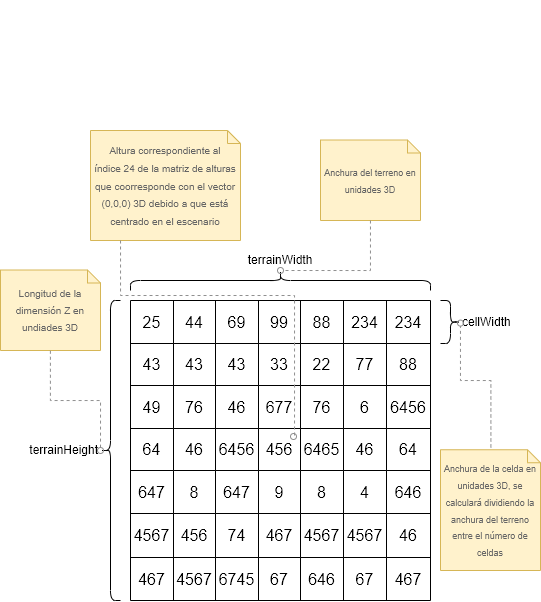
\includegraphics[width=10cm, keepaspectratio]{img/terrain.drawio.png}
  \caption{Diagrama de matriz de alturas.}
  \label{fig:terrainDrawio}
\end{figure}
Dado que el terreno está centrado en el vector \emph{(0,0,0)}, es importante tener en cuenta que el cálculo de la posición en el mundo \textsc{3D} estará centrado en torno al indice de la matriz que representa centro del escenario. 
Dado que la matriz empieza a contar los índices desde la esquina superior izquierda existe un desplazamiento con respecto al escenario que está centrado en el eje \emph{(0,0,0)}.
Para tener en cuenta este desplazamiento, calculamos el centro de la matriz dividiendo la anchura total del terreno por la mitad y sumando el resultado al eje x del vector 3D. 
Para determinar la columna correspondiente en la matriz, dividimos la posición \texttt{x} entre el ancho de cada celda y redondeamos el resultado para obtener un índice exacto. Esto nos dará la columna correspondiente en la matriz. 
De manera similar, calculamos la fila correspondiente en la matriz utilizando el eje Z. Estos cálculos nos proporcionarán la fila y columna adecuadas en la matriz de alturas.
En la figura \ref{formula:calculoIndiceAlturas} podemos ver las fórmulas de calculo de indices en columna y fila que acabos de describir.

Finalmente, es importante mencionar que estamos utilizando una representación de la matriz de alturas en formato de array unidimensional. Aunque conceptualmente es una matriz bidimensional, se almacena en una variable de tipo array de una sola dimensión. 
Para determinar el índice en el array al que corresponde una determinada fila y columna en la matriz, realizamos una operación básica para convertir el índice bidimensional en un índice unidimensional.
La fórmula utilizada para este cálculo se muestra en la Figura \ref{formula:calculoIndiceAlturas}. Esta fórmula nos permite acceder correctamente al valor de altura correspondiente en el array, teniendo en cuenta la relación entre la posición bidimensional y la representación unidimensional de la matriz de alturas.

Una vez obtenido el índice de la matriz, es necesario normalizar el valor correspondiente en el array de alturas. Dado que el array utiliza el tipo de dato \texttt{Uint16}, cuyo valor máximo es 65535, al dividir el valor obtenido se normaliza el rango de alturas entre \texttt{[0,1]}. Si se utiliza un factor de magnificación configurado en el componente, se puede obtener la altura real utilizada en el entorno 3D. Esta relación se explica en el contexto de la última fórmula en la Figura \ref{formula:calculoIndiceAlturas}.

En resumen para obtener la altura correspondiente a un vector de posición en el mundo 3D se realizan las siguientes operaciones:
\begin{enumerate}
	\item Se calcula la fila y la columna relacionada con el vector de posición 3D a través de las fórmulas descritas en la figura \ref{formula:calculoIndiceAlturas}.
	\item Se transforma la fila y la columna a un índice del array unidimensional de alturas.
	\item Se transforma el valor del array al valor normalizado usado por el componente, dando como resultado la altura pintada en el escenario.
\end{enumerate}

\subsection{Generación de datos geoespaciales de los edificios}
\label{subsec:buildingData}
Para extraer la información \gls{geoespacial} de los edificios, nos hemos basado en el servicio proporcionado por \textsc{Overpass}\footnote{\url{https://overpass-api.de/}}, el cual ofrece acceso a datos geoespaciales almacenados en la base de datos de \textsc{OpenStreetMaps}\footnote{\url{https://www.openstreetmap.org/}}. 
Overpass nos brinda una \textsc{API} que nos permite realizar consultas a la base de datos y también proporciona una herramienta en línea llamada \textsc{Overpass Turbo}\footnote{\url{https://overpass-turbo.eu/}}, que nos permite visualizar consultas a la \textsc{API}, así como visualizar y exportar los resultados de manera interactiva.
Inicialmente, consideramos cargar los datos en línea en tiempo real. Sin embargo, debido a que el formato del resultado de la consulta requería un preprocesamiento adicional y a la gran cantidad de entidades que se recuperaban en cada consulta, llegamos a la conclusión de que, para el prototipo, sería mejor trabajar con una cantidad reducida de entidades preprocesadas previamente y almacenadas localmente dando así prioridad al rendimiento de la aplicación.
Para descargarnos los datos haremos uso de \textsc{Postman}\footnote{\url{https://www.postman.com/}} y generaremos la siguiente petición para la \textsc{API}:

 \label{manual:consultaEdificios}
{\scriptsize
    \begin{verbatim}
    https://overpass-api.de/api/interpreter?
    data=(way[building]["building:levels"]
    (40.023417003380956,-4.204133836988655,40.744144594569384,-3.253816454176155);
    relation[building]["building:levels"]
    (40.023417003380956,-4.204133836988655,40.744144594569384,-3.253816454176155);
    );out;>;out skel qt;
    \end{verbatim}
}
Esto nos proporciona un archivo \textsc{XML} con todos los metadatos de los edificios en la zona del escenario de Madrid. El siguiente paso consistirá en convertir este archivo \textsc{XML} en un archivo \textsc{GEOJSON} que podamos utilizar para trabajar con él. Esto se debe a que la búsqueda de información en el formato de \textsc{OpenStreetMaps} es complicada debido a que los metadatos están distribuidos a través de identificadores y no se encuentran todos juntos en una única entidad, como sucede en el caso de \textsc{GEOJSON}.

Para llevar a cabo esta conversión, utilizaremos el proyecto \textsc{osmtogeojson}\footnote{\url{https://github.com/tyrasd/osmtogeojson}}, una biblioteca de código abierto disponible en \textsc{GitHub} que nos permitirá convertir los datos de formato \textsc{OpenStreetMap} (\textsc{OSM}) al formato \textsc{GEOJSON}. 
Para realizar este proceso, simplemente debemos instalar la biblioteca utilizando \textsc{Node.js} y ejecutar su \emph{script} correspondiente.

\label{manual:osmtogeojson}
{\scriptsize
    \begin{verbatim}
    npm install -g osmtogeojson
    osmtogeojson data\buildings.xml > data\buildings.geojson
    \end{verbatim}
}

\subsection{Geometria edificio}
\label{subsec:buildingGeometry}
En esta sección, vamos a describir brevemente la implementación de la generación de edificios utilizando la información proporcionada por la \textsc{\gls{API}} de \textsc{Overpass}.

El gestor de alturas utiliza un archivo geoespacial en formato \textsc{GEOJSON} para representar los edificios. Cada edificio se define usando una lista de coordenadas geoespaciales en el sistema de referencia \textsc{WGS84}, que describe su contorno. En ocasiones también se incluye un metadato que indica el número de pisos del edificio dependiendo la zona que consultemos, sobre todo encontraremos más metadatos de alturas en ciudades grandes. 
Para la generación de la geometría del edificio, necesitaremos la lista de coordenadas ya convertida al espacio \textsc{3D} utilizando nuestro conversor descrito en la sección \ref{subsec:mapConversion}, la altura del terreno y la altura del edificio calculada a partir del número de pisos.

Para calcular la altura del terreno, obtenemos el \gls{centroide} de la lista de puntos que definen el contorno del edificio. Luego, aplicamos las fórmulas descritas en \ref{formula:calculoIndiceAlturas} para determinar la altura del terreno en el punto del centroide.

En nuestra implementación, comenzamos creando una geometría bidimensional en \textsc{Three.js} a partir de la lista de coordenadas del edificio. Sin embargo, surge un problema al realizar la extrusión, ya que las coordenadas que utiliza la API de \textsc{Three.js} para extruir una forma son en 2D y al devolver la geometría 3D tendrá la siguiente forma \texttt{(x, y, 0)}, cuando en realidad deberían ser \texttt{(x, 0, y)}. 
Por lo tanto, después de crear la forma, aplicamos una rotación de 90 grados alrededor del \emph{eje X} para colocar el edificio en su posición original. Luego, ajustamos la altura del edificio aplicando una traslación en el \emph{eje Y} que incluye la altura del terreno y la altura del edificio. De esta manera, el edificio queda correctamente posicionado y anclado al terreno.

\begin{figure}[h]
  \centering
  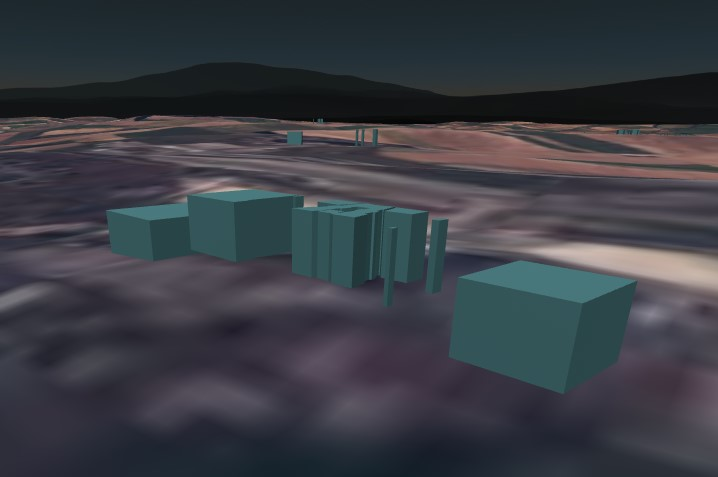
\includegraphics[width=10cm, keepaspectratio]{img/buildings.jpg}
  \caption{Edificios extruidos sobre el terreno.}
  \label{fig:buildings}
\end{figure}
\subsection{Componente gestor de altura de cámara}
\label{subsec:cameraHeight}
Este componente se configura en la entidad agrupadora que contiene la cámara principal y es responsable de ajustar la altura a medida que el usuario se desplaza por el escenario. Es un componente que simula el desplazamiento sobre la superficie del terreno para crear una experiencia inmersiva al caminar sobre un terreno con relieve.

La altura del personaje se mantiene constante de manera relativa con respecto a la altura del terreno. En otras palabras, la posición vertical del personaje se ajusta para mantener una altura constante con respecto al terreno.
Es importante tener en cuenta que el tamaño del personaje no sigue la misma escala que el escenario. Esto se debe a que el objetivo de la aplicación es visualizar datos a gran escala, y si el personaje principal se estableciera en la misma escala, sería difícil que se desplace rápidamente en un escenario que representa cientos de kilómetros. Estas diferencias de escala y velocidad del personaje son configurables.

El componente inicialmente se suscribe al cargador del terreno para establecer la altura correspondiente a la posición inicial del personaje una vez que el terreno se haya inicializado. También crea una función de \emph{throttledFunction}, como se explica en \ref{sec:mainScene}, para no penalizar el rendimiento por introducir lógica en la función \texttt{tick}. Por lo tanto se ha configurado la función para que actualice la posición de la cámara cada 200 ms, lo que implica que la altura de la cámara se actualiza 5 veces por segundo. Esto proporciona una experiencia satisfactoria con una pequeña penalización en el rendimiento.

Para calcular la altura, se obtiene el vector actual del objeto 3D de la cámara y del objeto que agrupa al personaje y que contiene la cámara. Para obtener la posición real de la cámara en el mapa, se realiza un cálculo teniendo en cuenta la configuración establecida en el proyecto para el personaje principal, como se muestra en la figura \ref{codigo:rig}.\\
\begin{figure}[h]
\centering
\begin{minted}[fontsize=\scriptsize, frame=single, numberblanklines=false,breaklines]{html}
<!-- Camera -->
<a-entity id="rig" position="0 0 0" movement-controls terrain-height>
  <a-entity id="camera" hud camera look-controls="reverseMouseDrag:false" cursor="rayOrigin: mouse; fuse: false"
    raycaster="far: 4000; objects: .clickable" position="0 0 0" toolbar3d>
  </a-entity>
  <a-entity id="left-hand" oculus-touch-controls="hand: left" laser-controls="hand: left"
    raycaster="far: 4000; objects: .clickable"></a-entity>
  <a-entity id="right-hand" oculus-touch-controls="hand: right" laser-controls="hand: right"
    raycaster="far: 4000; objects: .clickable"></a-entity>
    <a-entity id="cameraOnBoarEntity" camera="active: false" camrender="cid:cameraOnBoard;fps:25" position="0 0 0"
    rotation="0 -180 0"></a-entity>
</a-entity>
\end{minted}
\caption{Código que configura el personaje principal, compuesto por la cámara y las manos.
\label{codigo:rig}
}
\end{figure}
En la configuración, podemos observar que el esqueleto del personaje principal contiene un componente \emph{movement-controls} del proyecto \textsc{A-Frame extras}\footnote{\url{https://github.com/c-frame/aframe-extras/tree/master}}, que permite un movimiento del personaje compatible con el teclado y los joysticks de varios dispositivos de realidad aumentada, como las gafas de realidad aumentada \textsc{Oculus}.

Por otro lado, la cámara principal, que representa la cabeza del personaje, contiene el componente \emph{look-controls} de \textsc{A-Frame}, que nos permite mover la cabeza tanto con el ratón como con los sensores de posición de las gafas de realidad aumentada.
Debido a esto, la posición real de la cámara es relativa al componente del personaje principal. Es por eso que, en nuestro cálculo, extraemos ambos vectores y los sumamos para obtener la posición absoluta de la cámara en el escenario.

Una vez calculada la posición de la cámara principal en el escenario, utilizamos la instancia del gestor de alturas descrito en la sección~\ref{subsec:heightManager} para llamar a la función que nos devuelve la altura a través de un vector 3D del escenario. Con esa altura, sumada a la altura del personaje, establecemos la coordenada \texttt{Y} del vector del objeto \textsc{3D} de la cámara, ajustando la altura en función de la posición en el escenario un total de 5 veces por segundo.

\section{Gestión de acceso a los datos}
\label{sec:data}
En esta sección, vamos a analizar los componentes clave de la arquitectura principal encargados del acceso a los datos. En el prototipo desarrollado, se pueden configurar dos tipos de comportamientos.

El primero se refiere a la escena principal funcionado como una representación de datos en caché. En este caso, se muestra un histórico de datos obtenidos a través de la pieza responsable de guardar datos de la \textsc{API} dentro del prototipo o de otra fuente de datos históricos. 
El único requisito es que estos datos mantengan el mismo formato \textsc{\gls{JSON}} proporcionado por la \textsc{API} de \textsc{OpenSky}. Sin embargo, en el futuro, se podrían desarrollar fácilmente componentes adicionales que puedan leer otros formatos de datos, ya que toda la información está referenciada a la misma clase, la cual es precargada por el módulo de configuración. Por lo tanto, si cambian las posiciones de la información proveniente de otro servidor, solo se requeriría reconfigurar las posiciones en el archivo de configuración que precarga la escena.

El segundo comportamiento se refiere a la representación en tiempo real del tráfico aéreo. En este caso, los datos provienen directamente del servicio\textsc{ OpenSky REST API}, que nos proporciona datos \textsc{ADS-B} en tiempo real. Estos datos se representarán en el escenario, lo que permitirá mostrar el espacio aéreo en un entorno \textsc{3D} en tiempo real. Esta funcionalidad resulta especialmente útil como punto de partida para aplicaciones de control de espacios aéreos.
\subsection{Datos caché de vuelo}
\label{subsec:datosCacheVuelo}
En esta sección, vamos a describir cómo se gestiona la caché a través de la clase \emph{FlightCacheData}, que se encuentra en el archivo \emph{FlightCacheData.js} dentro del módulo de gestión de datos.
Estos objetos se instancian cuando un vuelo aparece en el escenario y se mantienen siempre y cuando el vuelo esté presente en cada lectura de datos de la \textsc{API}. Actúan como objetos \texttt{\gls{DTO}} (\emph{Data Transfer Object}) para mantener el estado del avión.
Estos objetos son necesarios para el cacheo de la posición antigua dentro del escenario, lo cual es crucial para generar animaciones que proporcionen un movimiento fluido de los aviones. 
Además, cada vez que se actualiza la posición de un avión, se emite un evento al componente responsable de pintar el trayecto del vuelo (descrito en la sección \ref{subsec:track}). De esta manera, el componente puede actualizar su geometría y mostrar el trayecto de los aviones desde su entrada en el escenario hasta su posición actual.

Como ya se describió en la sección \ref{subsec:movimientoFluido}, estos objetos se almacenan en un mapa indexado a través de su identificador para que su recuperación sea eficiente, servirán para mantener el estado de un vuelo específico en el escenario. Esto permite que el gestor del escenario genere una animación utilizando el vector de la caché y el nuevo vector leído de la API para lograr un movimiento fluido, y también actualiza la geometría responsable de representar el trayecto del avión en el escenario mediante un evento emitido sobre el escenario.
\subsection{Objeto de acceso a datos ADS-B (\gls{DAO})}
\label{subsec:dao}
El objeto de acceso a datos, comúnmente conocido como \texttt{\gls{DAO}} (\emph{Data Access Object}), es el objeto responasable de la obtención de los datos ADS-B. Como se muestra en la figura \ref{fig:dao}, el \texttt{DAO} accede al gestor de configuración para verificar si está configurado para acceder en tiempo real o utilizar datos en caché. 
En el caso de estar configurado para usar datos en caché, el \texttt{DAO} consulta al gestor de configuración la carpeta y el índice desde donde debe comenzar a leer. En cada evento de actualización, el \texttt{DAO} lee un archivo \textsc{\gls{JSON}} de la carpeta especificada y lo proporciona al gestor principal de la escena.

Si la configuración del \texttt{DAO} está establecida en tiempo real, se realizará una petición a una \textsc{API REST} para obtener los datos en formato \textsc{JSON}. El \texttt{DAO} consultará al módulo de configuración para obtener el usuario y la contraseña necesarios para autenticarse en la \textsc{API}. Es importante destacar que la API nos permite realizar consultas dentro de una zona delimitada por coordenadas geodésicas. 
Por lo tanto, la petición se realizará dentro de los límites geodésicos establecidos en la configuración del escenario. La respuesta \textsc{JSON} de la \textsc{API} contendrá los vuelos que se encuentren dentro de la escena especificada.

El gestor principal de la escena utiliza los datos proporcionados por el \texttt{DAO} para crear las instancias en caché de cada vuelo. Como se muestra en la figura \ref{fig:dao}, el gestor principal mantiene un mapa que almacena la caché de los vuelos, indexados por su identificador único de vuelo (\textsc{ICAO24}). En cada evento temporal, el gestor principal se encarga de mantener la tabla de caché. Si un vuelo no ha sido actualizado, se elimina de la tabla. Si ha sido actualizado, se actualiza la instancia de datos en caché correspondiente. Si el vuelo no existe en la tabla, se inserta en ella. De esta manera, la tabla de caché representa de manera precisa los vuelos presentes en la escena en ese momento específico.

\begin{figure}[h]
  \centering
  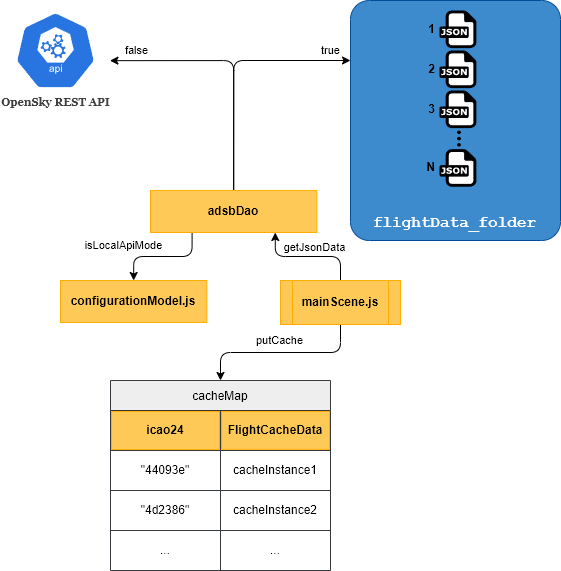
\includegraphics[width=10cm, keepaspectratio]{img/adsbDao.png}
  \caption{Diagrama del objeto de acceso a datos \textsc{ADS-B} (\texttt{DAO}).}
  \label{fig:dao}
\end{figure}

\subsection{Consulta y almacenamiento de datos a la carpeta caché}
\label{subsec:obtencionCache}
Para asegurar el correcto funcionamiento del componente de acceso a los datos mencionado en la sección anterior \ref{subsec:dao}, es necesario contar con la implementación de una pieza responsable del almacenamiento de los datos en una carpeta de caché local. Así posteriormente, el \texttt{\gls{DAO}} puede consultar esta carpeta en caso de que esté configurado en el modo local.
Este componente está implementado en \textsc{JavaScript} y se ejecuta en el entorno de \textsc{Node.js}. Su función principal es cargar previamente la configuración de un escenario específico, que incluye parámetros como el rectángulo geodésico para la obtención de datos y el intervalo de tiempo en el que se debe establecer el temporizador para realizar una petición a la \textsc{API} en cada evento. Además, este componente se encarga de almacenar el resultado de cada petición en un archivo dentro de la carpeta de caché, como se muestra en la figura \ref{fig:saveApiData}.
\begin{figure}[h]
  \centering
  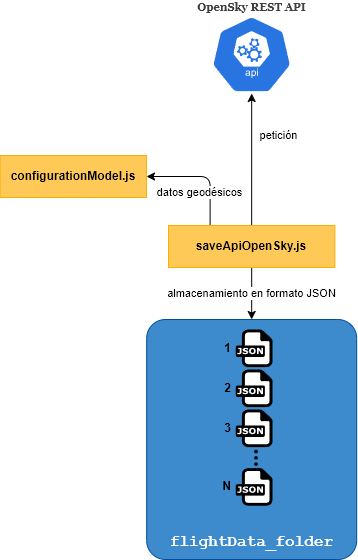
\includegraphics[width=9cm, keepaspectratio]{img/almacenamientoCache.drawio.png}
  \caption{Diagrama de consulta y almacenamiento de datos ADS-B en caché.}
  \label{fig:saveApiData}
\end{figure}
\begin{figure}[h]
  \centering
  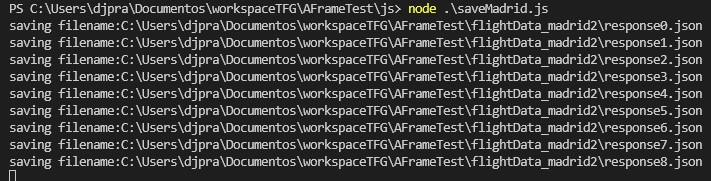
\includegraphics[width=9cm, keepaspectratio]{img/captura_datos_madrid.jpg}
  \caption{Ejecución con Node.js del almacenamiento de datos ADS-B en caché.}
  \label{fig:capturaDatosCache}
\end{figure}

Como podemos apreciar en la figura \ref{fig:capturaDatosCache} , en cada petición almacenamos en la carpeta local que usaremos de cache, un fichero \textsc{\gls{JSON}} con los vectores de posición de los vuelos en ese instante temporal.
Estos ficheros podrán ser leídos por el \texttt{DAO}, el componte anteriormente descrito en la sección \ref{subsec:dao}.
\clearpage
\section{Gestión de la interfaz de usuario}
\label{sec:gui}
En esta sección, vamos a examinar las soluciones y componentes implementados para la interacción del usuario con la aplicación, tanto en el modo de escritorio como en el modo de realidad virtual. En el modo de realidad virtual, se hace uso de gafas y mandos como las gafas \textsc{Oculus VR} para manipular las entidades en el entorno tridimensional.

El objetivo principal de todos los componentes desarrollados en esta aplicación es proporcionar al usuario la capacidad de consultar toda la información presente en la escena y visualizarla de una manera que sea equivalente a las posiciones reales de las entidades en el mundo real, pero al mismo tiempo, que sea manejable por el usuario. Esto significa que, aunque en el mundo real no podemos ver con claridad una entidad que represente un avión situado a 60 km de distancia, la aplicación tiene como objetivo seguir permitiendo el acceso a todas las entidades del escenario, independientemente de su ubicación en relación al usuario.
\subsection{Entidades en ampliación al alejarse}
\label{subsec:hover-scale}
Uno de los desafíos encontrados en la usabilidad de la aplicación se refiere a la selección de aviones para visualizar sus datos. Dado que los aviones en la realidad se encuentran a distancias significativas en términos de altura y dimensiones del escenario, sin aplicar técnicas para visualizar objetos distantes, sería imposible seleccionarlos y visualizarlos correctamente.

Para abordar este problema, se ha optado por una solución que sacrifica un poco de realismo dentro del escenario. Cuando un objeto supera cierto umbral de distancia, se aplica un proceso de ampliación que simula que el tamaño del símbolo del avión se mantiene más o menos constante. Con esta solución, facilitamos al usuario la capacidad de seleccionar aviones distantes. Puedes observar las capturas de pantalla que ilustran la escena con el componente de ampliación y sin el en las figuras \ref{fig:con-hover} y \ref{fig:sin-hover}.
\begin{figure}[h]
	\begin{align*}
		\text{{Factor de Ampliacición}} = \left(\frac{{\text{{distancia}} - \text{{distancia umbral}}}}{{\text{{divisor ampliación}}}}\right) + 1\\
	\end{align*}
	\caption{Calculo del factor de ampliación en función de la distancia.}
	\label{formula:ampliación}
\end{figure}
\begin{figure}[h]
  \begin{minipage}[t]{0.5\linewidth}
    \centering
    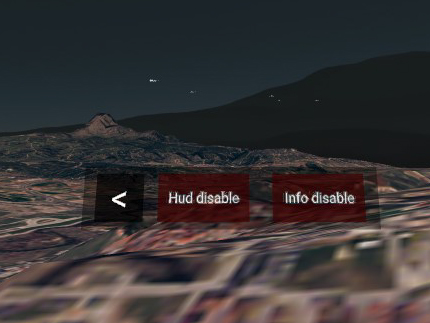
\includegraphics[width=7.5cm, keepaspectratio]{img/sin_hover.jpg}
    \caption{Aviones sin ampliación.}
    \label{fig:sin-hover}
  \end{minipage}%
  \begin{minipage}[t]{0.5\linewidth}
    \centering
    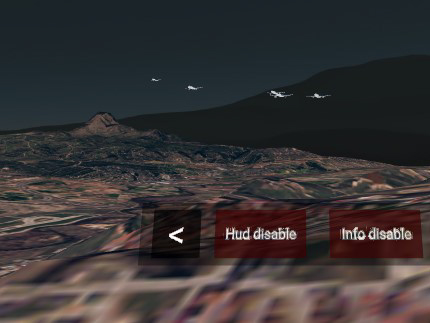
\includegraphics[width=7.5cm, keepaspectratio]{img/con_hover.jpg}
    \caption{Componente de ampliación.}
    \label{fig:con-hover}    
  \end{minipage}
\end{figure}
El componente se agrega a cada entidad que representa un vuelo y calcula la distancia entre la cámara principal y la entidad. Si la distancia supera un umbral configurado, se aplica un escalado a la entidad en cada repintado. La fórmula utilizada para el escalado se muestra en la figura \ref{formula:ampliación}. Esta fórmula calcula un factor de ampliación en función de la distancia, donde se asegura que el factor sea 1 en el umbral, lo que significa que no se realiza ningún escalado. A medida que la distancia aumenta, el factor se incrementa linealmente, y se puede ajustar el incremento mediante un factor divisor configurable. 
Todos estos parámetros, como el divisor del factor de ampliación y la distancia a partir de la cual se comienza a aplicar el escalado, son configurables, lo que brinda al usuario la capacidad de ajustar la visualización de los tamaños en diferentes distancias según sus preferencias.

\subsection{Componente de información contextual interactiva}
\label{subsec:tooltip}
En esta sección, describiremos el componente encargado de mostrar los metadatos de las entidades geoespaciales presentes en el escenario. Dado que el objetivo de la aplicación es visualizar información de entidades georeferenciadas, resulta interesante desarrollar un componente que inserte texto sobre las entidades del escenario que contengan metadatos.

Como se explicó anteriormente en la sección \ref{subsec:buildingGeometry}, al procesar la información de la capa de edificios extraída de los datos de \textsc{OpenStreetMap}, tenemos la capacidad de extraer los metadatos asociados a cada edificio generado. 
Por lo tanto, se ha creado un componente al cual se le puede proporcionar un texto como argumento y tiene la responsabilidad de generar un texto que siempre mire hacia la cámara y se posicione sobre la entidad correspondiente. 
Este texto solo es visible cuando el ratón o el \emph{raycaster} están posicionados sobre la entidad. Además, el componente genera un material de color rojizo para indicar el elemento seleccionado del cual se muestra la información. De esta manera, podemos visualizar los metadatos de edificios, como se muestra en la figura \ref{fig:tooltip}.

\begin{figure}[h]
  \centering
  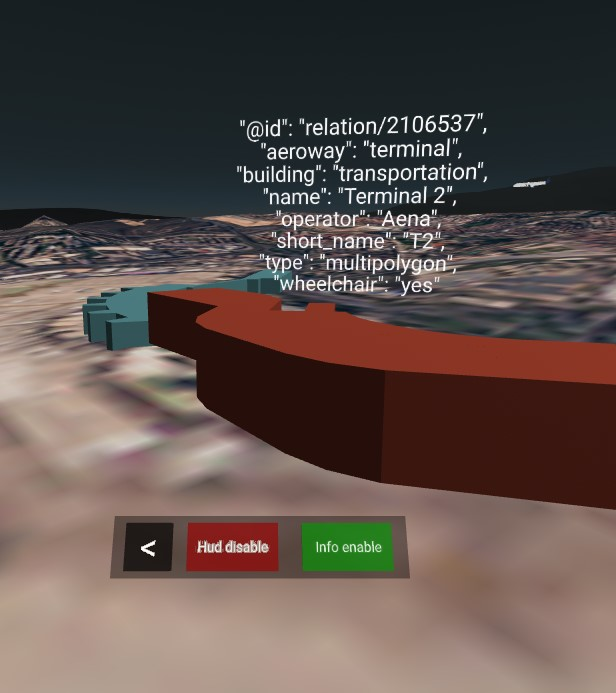
\includegraphics[width=8cm, keepaspectratio]{img/tooltip.jpg}
  \caption{Componente información contextual mostrando metadatos de la terminal.}
  \label{fig:tooltip}
\end{figure}
Como veremos más adelante, este componente tiene la capacidad de ser activado o desactivado mediante eventos enviados a través de la barra de herramientas (vease la sección \ref{subsec:toolbar3d}), la cual está presente como una interfaz de usuario en la cámara principal. Esto brinda al usuario la flexibilidad de controlar la visualización de los metadatos según sus necesidades y preferencias.

\subsection{Componente barra de herramientas de la interfaz de usuario}
\label{subsec:toolbar3d}
En esta sección, exploraremos el componente que acompaña al usuario y permite habilitar o deshabilitar funcionalidades. La barra de herramientas es una entidad 3D que se despliega como un \textsc{\gls{HUD}} \emph{(Head-Up Display)} en forma de pantalla frontal de visualización. Proporciona al usuario una interfaz para interactuar con las diversas funcionalidades de la aplicación.

Dado que nos encontramos en un entorno 3D, hemos implementado la barra de herramientas como un componente 3D dentro de la escena, anclado a la cámara principal. Sin embargo, nos hemos enfrentado al desafío de que esta barra puede resultar molesta al bloquear parte de la vista del usuario. Para solucionar este problema, hemos diseñado el componente de manera que pueda plegarse y arrastrarse, brindando al usuario la capacidad de colocarlo en una posición menos intrusiva y ocupando un espacio mínimo en la pantalla.
En la figura~\ref{fig:toolbarDesplegada} podemos ver la barra de herramientas en su tamaño desplegado mientras que en la figura~\ref{fig:toolbarPlegada} se aprecia el poco espacio que ocupa una vez la plegamos.
\begin{figure}[h]
  \begin{minipage}[t]{0.5\linewidth}
    \centering
    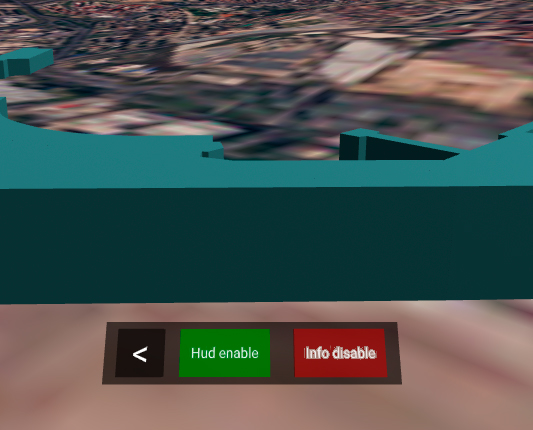
\includegraphics[width=7cm, keepaspectratio]{img/toolbarAbierta.jpg}
    \caption{Barra de herramientas desplegada.}
    \label{fig:toolbarDesplegada}
  \end{minipage}%
  \begin{minipage}[t]{0.5\linewidth}
    \centering
    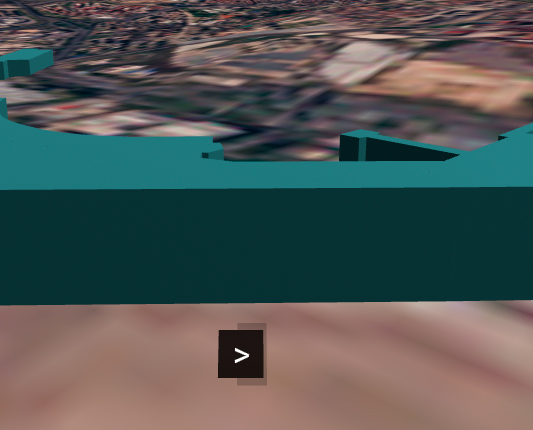
\includegraphics[width=7cm, keepaspectratio]{img/toolbarPlegada.jpg}
    \caption{Barra de herramientas plegada.}
    \label{fig:toolbarPlegada}    
  \end{minipage}
\end{figure}
\\La solución técnica implementada consiste en la creación de un componente que se configura dentro de la jerarquía de la cámara principal. Durante la inicialización de este componente, se agregan geometrías cuadradas de \textsc{A-Frame} de tipo \emph{a-plane} a la cámara principal para formar tanto el panel como los botones conmutables. 
Esto se puede observar en la figura que muestra la disposición de los componentes en la barra de herramientas (\ref{fig:toolbarComposition}).
\begin{figure}[h]
	\centering
	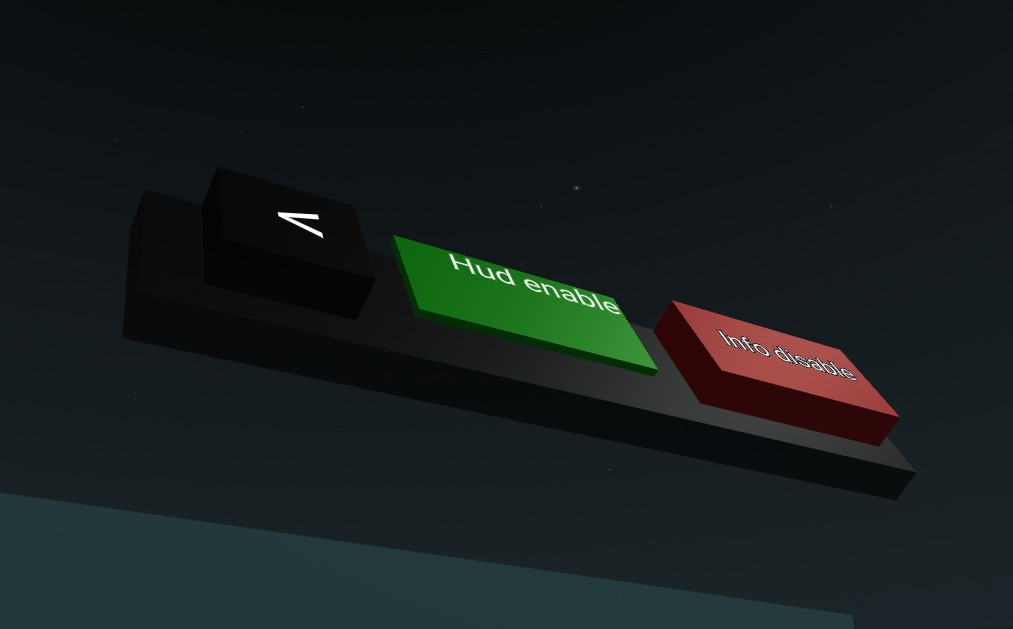
\includegraphics[width=8cm, keepaspectratio]{img/toolbarElementos.jpg}
	\caption{Maquetación del componente barra de herramientas.}
	\label{fig:toolbarComposition}
\end{figure}
La barra de herramientas está representada por un plano principal con transparencia, mientras que los botones se representan mediante tres planos adicionales con texto superpuesto. Estas geometrías planas tienen añadidos controladores de eventos para permitir la interacción con el usuario.\\
\begin{figure}[h]
	\centering
	\begin{minted}[fontsize=\scriptsize, frame=single, numberblanklines=false,breaklines]{javascript}
		createToolbarButton: function (id,width, height, text,texSize, position, toogle, enableFunction, disableFunction, enableColor, disableColor, enableText, disableText)
	\end{minted}
	\caption{función que genera los botón dentro de la barra de herramientas.
		\label{codigo:crearBoton}
	}
\end{figure}
Cada botón se crea mediante una función interna (ver Código \ref{codigo:crearBoton}) que recibe varios argumentos. Estos argumentos incluyen un identificador único utilizado para hacer referencia al botón en el contexto del \textsc{\gls{DOM}}, las dimensiones de la entidad que determinan su ancho y alto, el texto, la posición dentro de la barra de herramientas, si el botón es conmutable o no, la acción a ejecutar cuando el botón está activado y la acción a ejecutar cuando el botón está desactivado.
Además, se pueden especificar propiedades visuales para el botón cuando está en estado activado y cuando está en estado desactivado, como el color y el texto correspondiente. Esta configuración flexible y modular hace que nuestra barra de herramientas sea altamente reutilizable para otros proyectos y fácilmente extensible para añadir más funcionalidades dentro de la aplicación.
En la sección \ref{subsec:guiaBarra3d} mostramos un ejemplo de como reutilizar la barra de herramientas con mas detalles sobre la función que acabaos de describir.
Nuestra aplicación, haciendo uso del método anteriormente descrito nuestro componente barra de herramientas crea dos botones conmutables que permiten habilitar la funcionalidad de selección de aviones y visualizar su información a través de un panel \textsc{\gls{HUD}} que contiene acciones adicionales. Además, hemos incluido un botón que activa y desactiva la funcionalidad de texto contextual, como se describe en la sección anterior \ref{subsec:tooltip}.
\subsubsection{Animación de la barra de herramientas}
\label{subsec:animationToolbar}
Para lograr la funcionalidad de plegado, se han implementado animaciones que actúan sobre la escala y opacidad de los componentes de la barra de herramientas. Cuando el usuario presiona el botón de plegado, la barra de herramientas oculta los botones mediante una animación que los desvanece gradualmente a través de la opacidad. Luego, la barra de herramientas se comprime horizontalmente, lo que también afecta al botón de plegado, haciendo que se comprima en tamaño.
Para contrarrestar esta compresión, se realiza una animación inversa en el botón de plegado, expandiéndolo horizontalmente y restaurándolo a su tamaño original. Esto crea un efecto visual que contrarresta la compresión causada por el plegado de la barra de herramientas tal y como aclaramos en el diagrama \ref{fig:animationPlegado}.
\begin{figure}[h]
  \centering
  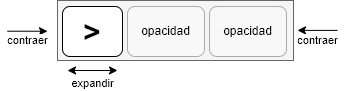
\includegraphics[width=7cm, keepaspectratio]{img/plegadoToolbar.drawio.png}
  \caption{Animaciónes para plegar la barra de herramientas.}
  \label{fig:animationPlegado}
\end{figure}
\subsection{Componente pantalla frontal de visualización (HUD)}
\label{subsec:hud}
El elemento \textsc{\gls{HUD}} es esencial en nuestra aplicación, ya que proporciona al usuario la visualización de datos de los aviones, así como funcionalidades adicionales relacionadas con los aviones seleccionados.
\begin{figure}[h]
  \centering
  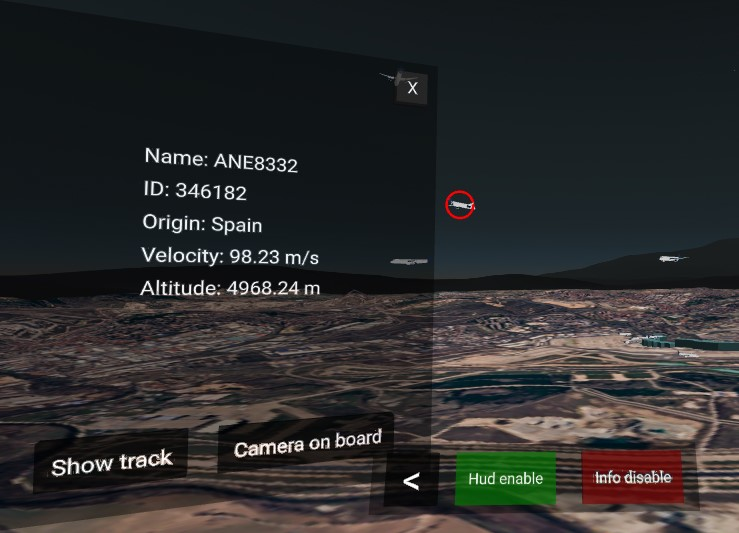
\includegraphics[width=8cm, keepaspectratio]{img/hud.jpg}
  \caption{Componente \textsc{HUD} con avión seleccionado.}
  \label{fig:hud}
\end{figure}

Uno de los principales objetivos de nuestra aplicación es permitir al usuario ver la información de los aviones en tiempo real o en diferido. Cuando habilitamos la funcionalidad del \textsc{\gls{HUD}} en la barra de herramientas, le brindamos al usuario la capacidad de seleccionar un avión y desplegar un panel informativo. Este panel contiene una serie de datos obtenidos a través de metadatos \textsc{ADS-B}, y se actualiza mediante eventos en cada consulta a la \textsc{API}.
En resumen, al activar la funcionalidad del \textsc{\gls{HUD}} en nuestra barra de herramientas, permitimos al usuario seleccionar aviones y ver información actualizada de los mismos, como la altura y velocidad, basada en metadatos \textsc{ADS-B} obtenidos a través de consultas a la \textsc{API}.
En la figura \ref{fig:hud}, podemos observar que cuando seleccionamos un avión, se agrega una entidad en forma de anillo que rodea al avión y siempre está orientada hacia la cámara. Esta entidad se desplaza junto con el avión y permite al usuario realizar un seguimiento visual del avión seleccionado. Además, proporcionamos al usuario dos acciones adicionales relacionadas con el avión seleccionado.

La primera acción consiste en visualizar el recorrido del avión en el escenario. Como se muestra en la figura \ref{fig:showTrack}, cuando un avión está seleccionado, se muestra un botón que habilita una línea azul que representa el trayecto que ha seguido el avión desde que ingresó al escenario hasta el momento actual. Esta línea muestra todas las posiciones que la entidad del avión ha ocupado durante su presencia en el escenario.

La segunda funcionalidad que ofrece el panel \textsc{\gls{HUD}} es la capacidad de visualizar una cámara de a bordo a través del panel. Esto brinda al usuario la experiencia de visualizar lo mismo que pueden ver los pasajeros del vuelo. La cámara de a bordo se proyecta en una pantalla que se despliega con una animación justo frente al panel \textsc{\gls{HUD}}, como se muestra en la figura \ref{fig:cameraOnBoard}.\\
\begin{figure}[h]
	\centering
	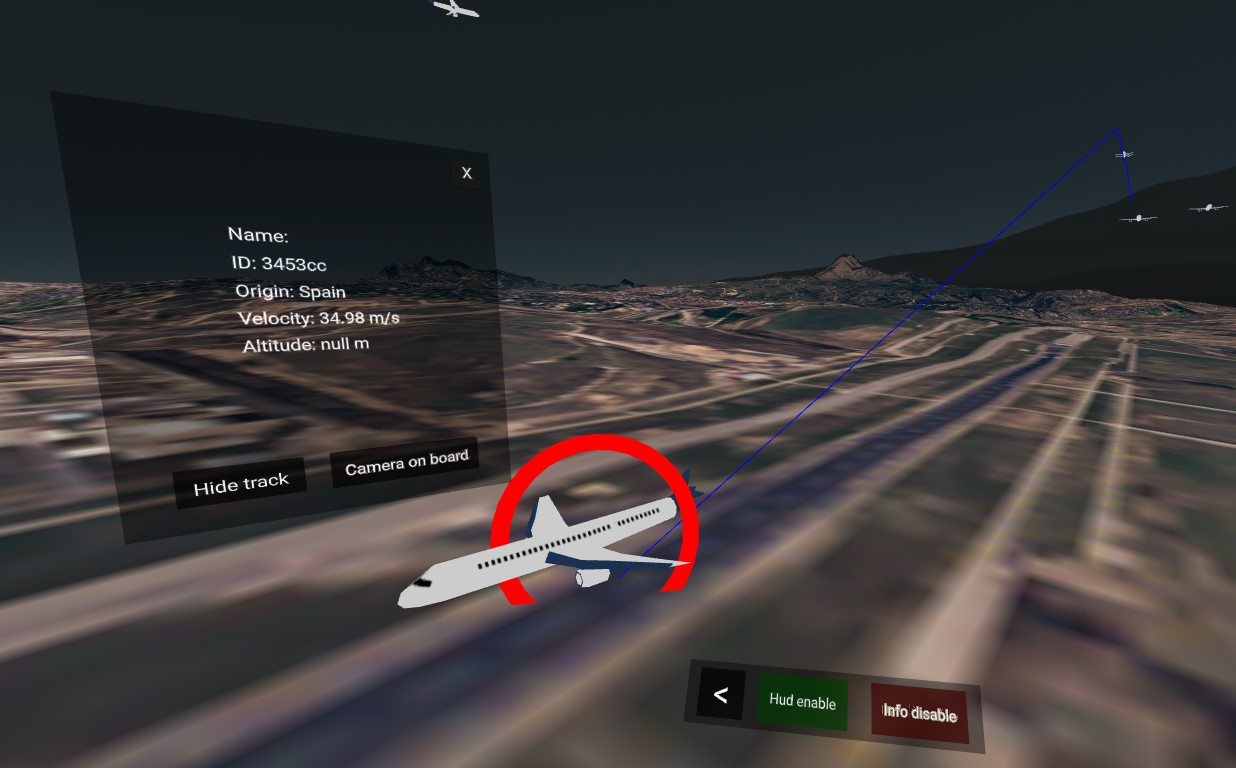
\includegraphics[width=8cm, keepaspectratio]{img/show_track.jpg}
	\caption{Trayecto del avión en el escenario.}
	\label{fig:showTrack}
\end{figure}
\begin{figure}[h]
  \centering
  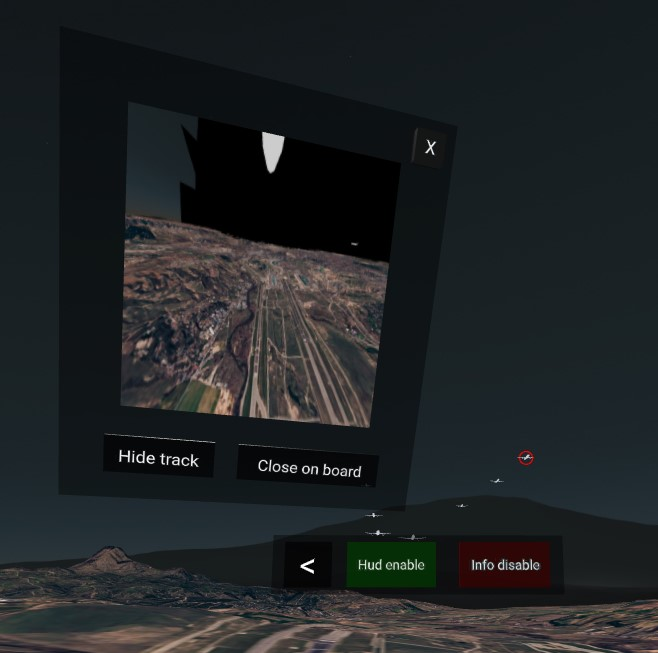
\includegraphics[width=8cm, keepaspectratio]{img/cameraOnBoard.jpg}
  \caption{Visualización de la cámara de a bordo sobre el HUD.}
  \label{fig:cameraOnBoard}
\end{figure}
\subsection{Desplazamiento de la barra de herramientas y pantalla frontal de visualización (HUD)}
\label{subsec:customDraggable}
Como mencionamos anteriormente, es de vital importancia brindar al usuario principal la capacidad de desplazar los componentes \textsc{\gls{HUD}} de nuestra aplicación. Por lo tanto, en esta sección abordaremos el componente que nos permite arrastrar y mover nuestros componentes \textsc{\gls{HUD}} a cualquier parte de nuestra área visual.
Tanto el componente pantalla frontal de visualización \ref{subsec:hud} como el componente barra de herramientas \ref{subsec:toolbar3d} configuran en su entidad principal el componente detallado en esta sección llamado \emph{custom-draggable} que será responsable de proporcionar al usuario usuario principal la capacidad de desplazar las entidades \textsc{HUD} donde no le moleste.

Implementar esta funcionalidad requirió mucho tiempo y esfuerzo, probando diversas estrategias e incluso explorando bibliotecas como \emph{A-frame-super-hands}\footnote{\url{https://github.com/c-frame/aframe-super-hands-component}}, aunque sin éxito. Esto se debe a que nuestro caso difiere significativamente de las aplicaciones convencionales.
El componente \emph{super-hands} está diseñado para agarrar y mover componentes que se encuentran en una posición absoluta, pero no está preparado para componentes que se encuentran en una posición relativa dentro de la estructura del esqueleto del usuario principal. Esta es la principal razón por la que no fue posible reutilizar ningún componente de las bibliotecas probadas, y se tuvo que desarrollar un componente propio. En este proceso, se encontró una solución ingeniosa para calcular la posición de manera eficiente, adoptando una estrategia diferente a cómo lo hacen las bibliotecas mencionadas. 
Además, se invirtieron muchas horas de investigación para garantizar que el componente fuera compatible tanto con gafas de realidad virtual como con un ratón convencional.\\
\begin{figure}[H]
  \begin{minipage}[b]{0.58\linewidth}
    En el archivo \emph{custom-draggable.js}, se ha creado un componente que permite arrastrar entidades que están contenidas dentro de la cámara principal. Es importante mencionar que en \textsc{A-frame}, cuando agregamos una entidad con geometría dentro de otra entidad, la posición de la entidad será relativa a su entidad padre. Nuestras entidades \textsc{\gls{HUD}} se basan en este concepto, por lo tanto, tanto la barra de herramientas descrita en la sección \ref{subsec:toolbar3d} como nuestra pantalla frontal de visualización descrita en la sección \ref{subsec:hud}, son entidades secundarias del esqueleto principal que representa al usuario (\emph{rig}) tal y como podemos ver en la figura \ref{fig:jerarquiaEntidadesRig}.
  \end{minipage}%
  \hfill
  \begin{minipage}[b]{0.4\linewidth}
    \centering
    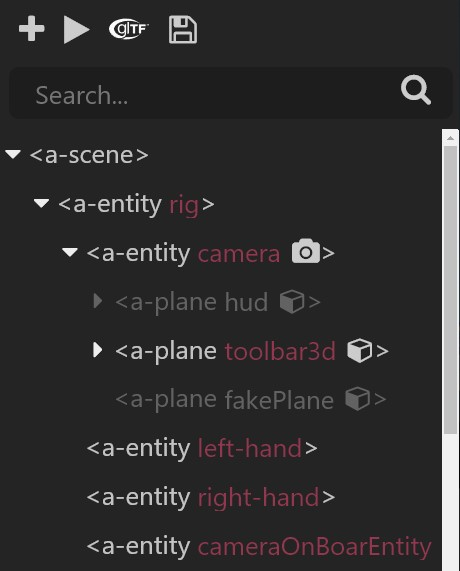
\includegraphics[width=6cm, keepaspectratio]{img/jerarquiaRig.jpg}
    \caption{Jerarquía de entidades.}
    \label{fig:jerarquiaEntidadesRig}    
  \end{minipage}
\end{figure}
Para permitir que los componentes que viajan con la cámara principal puedan ser arrastrados, vamos a aclarar el proceso. En primer lugar, es importante tener en cuenta que la complejidad radica en garantizar que el elemento se mueva siempre en el mismo plano, sin cambios en la profundidad, solo en las coordenadas horizontales y verticales.
Además, cuando arrastramos el componente con el ratón o el mando de las gafas de realidad virtual, es fundamental que siga el movimiento realizado para dar la sensación de arrastre.
Después de explorar diversas estrategias, llegamos a la conclusión de que la técnica más sencilla y eficiente es utilizar un \emph{\gls{raycaster}}. Un componente \emph{raycaster} es una herramienta fundamental en entornos \textsc{3D} que permite realizar intersecciones y detecciones de colisiones en la escena. Su funcionamiento se basa en el trazado de un rayo desde un origen en una dirección determinada. Cuando el rayo colisiona con las entidades envía eventos a los que los componentes pueden suscribirse.\\
\begin{figure}[h]
	\centering
	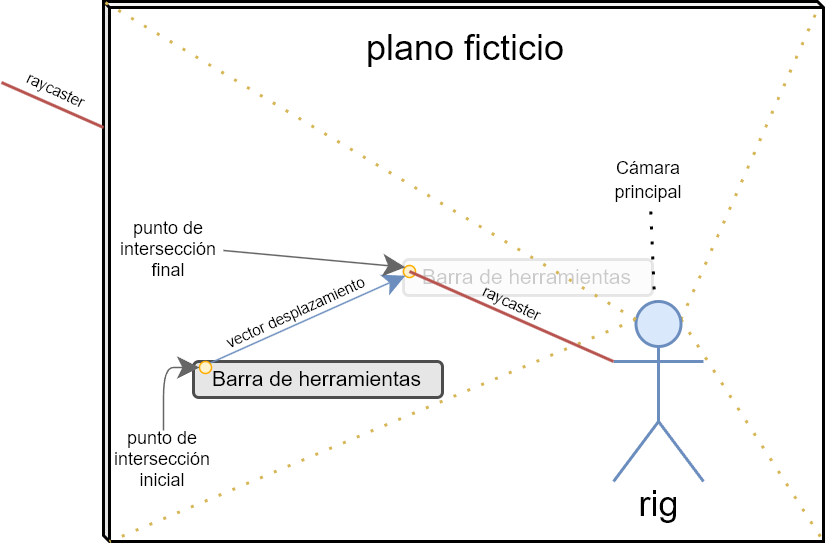
\includegraphics[width=10cm, keepaspectratio]{img/custom-draggable.png}
	\caption{Cálculo del vector desplazamiento de arrastre de entidades.}
	\label{fig:raycaster}
\end{figure}
Cuando recibimos el evento de presionar el botón para arrastrar en la entidad, guardamos el componente \emph{raycaster} que generó dicho evento, dentro de la instancia para recuperarlo en los eventos posteriores. 
También registramos la posición de intersección entre el \emph{raycaster} y el elemento \textsc{\gls{HUD}} y hacemos transparente la entidad para dar la sensación de que la tenemos agarrada. Después, cambiamos al estado de \texttt{presionado} y creamos una entidad plana ficticia e invisible que colocamos justo frente a la cámara principal, a la misma distancia que el elemento \textsc{\gls{HUD}} tal y como vemos en la figura\ref{fig:raycaster}. A partir de este punto, mientras estemos en el estado de "presionado" (es decir, arrastrando), en cada evento de la función \texttt{tick}, calculamos la intersección entre el plano ficticio y el \emph{raycaster} que generó el evento de agarre. A partir de esta intersección, determinamos el desplazamiento realizado por el controlador, que es un vector que contiene los incrementos de las coordenadas horizontales y verticales. Luego, convertimos este vector en uno relativo a la cámara y lo sumamos al vector de posición del elemento agarrado. De esta manera, logramos arrastrar y mover cualquier entidad que esté dentro de la jerarquía de la cámara en el plano deseado.
Finalmente, cuando soltamos el botón del mando o el ratón, cambiamos al estado de  \texttt{no presionado} para fijar la posición de la entidad y evitar que siga siendo desplazada en cada evento de la función \texttt{tick}.

Es importante destacar que todas las entidades \textsc{\gls{HUD}} contienen el componente \emph{look-at}\footnote{\url{https://github.com/supermedium/superframe/tree/master/components/look-at/}} de \textsc{A-Frame}, el cual garantiza que siempre estén orientadas hacia la cámara.
\subsection{Componente trayecto realizado por un vuelo}
\label{subsec:track}
El componente \emph{track}, contenido en el archivo \emph{track.js}, es un componente que se suscribe a los eventos del objeto \texttt{\gls{DTO}} \emph{FlightCacheData} descrito en el apartado \ref{subsec:datosCacheVuelo} y del panel \textsc{\gls{HUD}} descrito en el apartado \ref{subsec:hud}.
Es responsable de dibujar una línea que muestra el trayecto del avión en el escenario en caso de que el botón conmutable del \textsc{\gls{HUD}} que activa la funcionalidad del vuelo seleccionado esté habilitado. Este componente solo escucha eventos de su vuelo, por lo tanto, solo usará el \emph{tag} correspondiente al identificador de vuelo, escuchando eventos de los siguientes prefijos a través de eventos en el escenario:
\begin{itemize}
	\item \textbf{\emph{flightCacheData\_push\_}}: Evento recibido por el objeto \emph{FlightCacheData} para actualizar la lista de puntos que componen la línea.
	\item \textbf{\emph{flightCacheData\_show\_}}: Evento recibido por el panel \emph{HUD} emitido por el botón que activa la funcionalidad.
	\item \textbf{\emph{flightCacheData\_hide\_}}: Evento recibido al desactivarse el botón conmutable presente en el \emph{HUD}, que desactiva la funcionalidad.
	\item \textbf{\emph{flightCacheData\_clear\_}}: Evento emitido cuando el vuelo desaparece del escenario para borrar el elemento de la escena.
\end{itemize}
El dibujado del trayecto se realizará mediante la creación de una línea de \textsc{THREE.js} mediante un \emph{buffer} de puntos.
\chapter{Conclusiones}
\label{chap:conclusiones}
\section{Consecución de objetivos}
\label{sec:consecucion-objetivos}

Se ha desarrollado una plataforma de herramientas para la construcción de escenarios que brinda al usuario una experiencia más inmersiva en comparación con otras aplicaciones bidimensionales similares. He recreado parte de la funcionalidad ofrecida por las aplicaciones y servicios web de visualización de datos aeronáuticos, como se menciona en la sección \ref{sec:tecnosimilares}, pero en un entorno tridimensional mediante la implementación de un ecosistema de componentes que permite al usuario visualizar datos interactuando con el escenario aprovechando las tecnologías de realidad virtual.

He creado un conjunto de componentes que permiten ser reutilizados para otras aplicaciones de manera sencilla y he documentado como se pueden reutlizar, proporcionando una licencia para su reutilización o modificiación , se pretende que todos los avances de este proyecto puedan servir para futuras aplicaciones en otros proyecto, como es el ejemplo de todos los avances en la interfaz de usuario que pueden ser de gran utilidad independientenmente de la aplicación que se requiera realizar.

He creado dos escenarios que representan el entorno que rodea a los aeropuertos de \emph{Adolfo Suárez} Madrid y el aeropuerto de \emph{Châlons-Vatry} en Francia. Esto ha sido posible gracias a la creación de una plataforma sólida que permite reproducir escenarios que representen aviones y entidades georeferenciadas en cualquier parte del mundo y en las dimensiones necesarias. Esta plataforma proporciona una base sólida que se puede ampliar fácilmente en términos de funcionalidad.

Este ecosistema de componentes implementados en el prototipo, no se limita únicamente a aplicaciones de datos aéreos, sino que puede ser utilizado para cualquier tipo de aplicación \gls{gis}, brindando un escenario donde se puede consultar información georeferenciada. 
Por ejemplo, podría ser utilizado para la consulta de una red eléctrica por parte de una compañía que necesite visualizar entidades como acometidas, postes, cables de alta tensión, centros de transformación, entre otros, todo en un entorno tridimensional que permite consultar metadatos sobre una entidad seleccionada.
Esto proporciona una herramienta de gran valor añadido a un técnico, permitiendo visualizar donde se encuentra una avería o como planificar una obra para una ampliación de la red.

En resumen, esta plataforma es adecuada para cualquier tipo de aplicación de Sistemas de Información Geográfica que requiera visualizar entidades geoespaciales.

A nivel personal, ha sido una experiencia muy gratificante avanzar en cada iteración del proyecto y aprender nuevas bibliotecas y tecnologías que enriquecen mi conocimiento profesional. Cada obstáculo superado durante el desarrollo del proyecto ha representado una lección aprendida, la cual seguramente será de gran utilidad en mi futuro profesional.
\section{Aplicación de lo aprendido}
\label{sec:aplicacion}
\subsection{A través de la titulación}
\begin{itemize}
	\item \textbf{Fundamentos de la Programación}: Esta asignatura sentó las bases fundamentales de la programación, proporcionándome los conocimientos necesarios para desenvolverme en cualquier lenguaje de programación. Aprendí las herramientas principales utilizadas para implementar la lógica de negocio en diversos lenguajes de programación.
	\item \textbf{Aplicaciones Telemáticas}: Durante esta asignatura, adquirí experiencia en el desarrollo de aplicaciones del lado del \emph{Front-End}, utilizando lenguajes como \emph{JavaScript} y familiarizándome con el paradigma de la programación funcional. Además, amplié mis conocimientos en el desarrollo de componentes orientados a eventos, donde la lógica se encuentra desacoplada y la comunicación se realiza a través de eventos en el \emph{\gls{DOM}}.
	\item \textbf{Prácticas Académicas Externas}: Realicé mis prácticas en la empresa Indra, donde trabajé en un software de sistemas de información geográfica. Esta experiencia fue fundamental para mi desarrollo en el proyecto actual, especialmente en el aspecto \gls{geoespacial}. Adquirí conocimientos sobre proyecciones, datums y transformaciones necesarias para el manejo de ficheros binarios de alturas, donde una matriz define un espacio georeferenciado.
\end{itemize}
\subsection{De forma autodidacta}
\begin{itemize}
	\item \textbf{\emph{A-Frame}}: Durante el proceso de desarrollo, he adquirido conocimientos a través de la documentación de \textsc{A-Frame} \cite{aframedocs}. Esta documentación me ha permitido aprender a crear una amplia variedad de componentes y estrategias relacionadas con la solución de problemas típicos en programación de entornos tridimensionales.
	\item \textbf{\emph{Three.js}}: He adquirido conocimientos de forma autodidacta sobre cómo extruir geometrías complejas para la creación de edificios utilizando la librería \textsc{Three.js}.
	\item \textbf{\emph{Google Earth Engine}}: Con el fin de lograr escenarios más realistas, he tenido que investigar y aprender a utilizar por mi cuenta la \textsc{API} proporcionada por \textsc{Google} para obtener imágenes satelitales georreferenciadas. Estas imágenes me han permitido obtener texturas realistas para el terreno de mi aplicación.
	\item \textbf{\emph{Oculus Quest}}: He tenido que aprender a utilizar dispositivos de realidad virtual y adaptarlos a \textsc{A-Frame} para integrar los controladores en la aplicación. Esto ha permitido que el usuario pueda utilizar sus manos para interactuar con las entidades que representan la interfaz gráfica, como agarrar objetos y realizar acciones dentro de la aplicación.
	\item \textbf{\emph{OpenSky}}: He aprendido de forma autodidacta a utilizar la \textsc{API} de \textsc{OpenSky} mediante peticiones \textsc{REST} y a interpretar todos sus metadatos.
	\item \textbf{\emph{Node JS}}: He aprendido a utilizar \emph{npm} y \textsc{Node.js} para crear procesos por lotes que me permiten descargar datos de las \textsc{API} de \textsc{OpenSky} y almacenarlos en una caché local.
	\item \textbf{\emph{Overpass-api}}: Aprendí de manera autodidacta a utilizar las sentencias principales para consultar y obtener datos en los servidores de \textsc{OpenStreetMap}. Además, aprendí a descargar y convertir los datos para poder utilizarlos dentro del prototipo.
	\item \textbf{\emph{Leaflet}}: He aprendido a utilizar una librería para proyectar coordenadas y posteriormente realizar transformaciones afines, lo que me ha permitido realizar conversiones entre sistemas de referencia en el entorno 3D y sistemas geoespaciales.
	\item \textbf{\emph{Entorno de programación JavaScript}}: He aprendido a instalar y configurar un entorno de desarrollo utilizando el editor de código \textsc{VSCode} y un servidor local. Esto me ha permitido depurar el código \textsc{JavaScript} en tiempo de ejecución, lo que facilita la solución de errores y proporciona una plataforma sólida para el desarrollo.
	\item \textbf{\emph{\LaTeX}}: He aprendido a documentar utilizando \LaTeX y a instalar todos los plugins y complementos necesarios para la creación de una memoria técnica.
	\item \textbf{\emph{Draw.io}}: He aprendido a utilizar \emph{draw.io}\footnote{\url{https://app.diagrams.net/}} para crear diagramas que ayuden a los lectores de mi memoria a comprender mejor el contenido.
\end{itemize}
\section{Trabajos futuros}
\label{sec:trabajos_futuros}
El desarrollo de una aplicación es un proceso continuo, ya que siempre existen aspectos que se pueden mejorar y nuevas funcionalidades que se pueden añadir. Por esta razón, a continuación enumeraremos una serie de mejoras y nuevas funcionalidades que podrían aplicarse al prototipo en el futuro.

Estas mejoras y funcionalidades se han dividido en dos secciones según su complejidad. Los evolutivos complejos son tareas que requieren una estimación de tiempo prolongado o el desarrollo de varios componentes, mientras que los evolutivos sencillos son tareas simples que aportan un gran valor al proyecto con un costo temporal reducido. Cabe destacar que el prototipo está preparado para recibir modificaciones de manera sencilla.
\subsection{Evolutivos sencillos}
\begin{enumerate}
	\item Lectura de varios ficheros de edificios, daría mas versatilidad a la carga de edificios, siendo posible guardar varios ficheros por cada consulta, y que el software cargue todos los ficheros presentes en la carpeta configurada, de esta manera podemos dividir las entidades geoespaciales clasificandolas por tipo y comenzar a añadir incluso datos que no sean solo edificios.
	\item Añadir un conmutable a la barra de herramientas que active la funcionalidad de mostrar en un \textsc{HUD} las coordenadas geodésicas en las que se encuentra el usuario.
	\item Añadir un botón conmutable en la barra de herramientas que desactive el componente gestor de altura de la cámara permitiendo volar al usuario para visualizar otra perspectiva diferente del escenario.
	\item Realizar un componente que limite al usuario poder desplazarse fuera del escenario.
	\item Añadir un botón conmutable en la barra de herramientas que desactive el componente que amplifica los aviones con la distancia para tener una visualización más real cuando el usuario lo requiera.
	\item Una funcionalidad adicional de alto valor añadido sería la inclusión de una interfaz gráfica que permita al usuario ingresar un identificador de vuelo y seleccionar el avión correspondiente en la escena. Esto brindaría al usuario la capacidad de consultar información sobre los vuelos directamente desde la visualización 3D.
	\item Se puede implementar fácilmente que el gestor de terreno lea un archivo \textsc{JSON} que permita configurar entidades mediante una posición en el sistema de coordenadas \textsc{WGS84}, un texto informativo y un archivo \emph{gltf} que represente el modelo de esa entidad. De esta manera, se pueden cargar y añadir modelos \textsc{3D} de edificios importantes o monumentos al terreno añadiendo más realismo. Esto permite que el usuario configure de manera sencilla dichas entidades sobre el terreno y además proporcione información adicional cuando son seleccionadas por el usuario.
\end{enumerate}
\subsection{Evolutivos complejos}
\begin{enumerate}
		\item Se ha detectado que en escenarios grandes con velocidades de desplazamiento lentas ayudaría mucho añadir un conmutable a la barra de herramientas que despliegue un panel con el mapa visto desde arriba y nos permita seleccionar un punto del escenario donde desplazar al usuario de un salto.
		\item Usar estimaciones con las marcas de tiempo de los vectores de posición de \textsc{OpenSky} para hacer estimaciones reales de si las muestras nuevas.
		Si la nueva muestra tiene un intervalo temporal más pequeño que el utilizado por la aplicación, la posición mostrada reflejará un desplazamiento menor al real, lo que dará la sensación de que el avión se frena y luego acelera repentinamente en la siguiente muestra. En ese caso, podemos utilizar la información de la velocidad para descartar la posición y realizar una estimación basada en el trayecto y la velocidad del avión.
		\item Una mejora interesante sería habilitar la navegación entre escenarios directamente desde la aplicación. Sería muy útil comenzar la escena con una vista panorámica aérea en una escala amplia, similar a lo que hacen aplicaciones como \emph{FlightRadar24} ó \emph{Plane Finder}. Podríamos superponer entidades rectangulares transparentes que representen las áreas de los escenarios disponibles. Cuando el usuario pase el ratón por encima de una de estas entidades, podría seleccionarla y dirigirse a la aplicación correspondiente de ese escenario, manteniendo la misma marca temporal si se está visualizando la aplicación en el modo datos cacheados. Esta funcionalidad proporcionaría una manera atractiva y global de visualizar todos los escenarios disponibles para ejecutar.
\end{enumerate}


% Las siguientes dos instrucciones es todo lo que necesitas
% para incluir las citas en la memoria
\nocite{*}
\bibliographystyle{abbrv}
\bibliography{memoria}
% memoria.bib es el nombre del fichero que contiene
% las referencias bibliográficas. Abre ese fichero y mira el formato que tiene,
% que se conoce como BibTeX. Hay muchos sitios que exportan referencias en
% formato BibTeX. Prueba a buscar en http://scholar.google.com por referencias
% y verás que lo puedes hacer de manera sencilla.
% Más información: 
% http://texblog.org/2014/04/22/using-google-scholar-to-download-bibtex-citations/

\printglossaries
\newglossaryentry{3D}
{
	name=3D,
	description={
		Se refiere a la representación tridimensional de objetos o entornos en un espacio virtual. En el contexto de gráficos y visualización, el término 3D se utiliza para describir la capacidad de representar objetos con altura, anchura y profundidad, añadiendo así una dimensión adicional a la imagen o escena.
	}
}
\newglossaryentry{API}
{
	name=API,
	description={
		Siglas de ''Application Programming Interface'' (Interfaz de Programación de Aplicaciones). Se refiere a un conjunto de reglas y protocolos que permiten la comunicación y la interacción entre diferentes software o componentes de un sistema. Una API define las formas en que los programas pueden solicitar servicios o funcionalidades de otro software y cómo pueden intercambiar datos entre sí
	}
}
\newglossaryentry{framework}
{
	name=Framework,
	description={
		Conjunto estructurado de herramientas, bibliotecas, componentes y estándares que proporciona una base para el desarrollo de software
	}
}
\newglossaryentry{OpenGL}
{
	name=OpenGL,
	description={Una API de gráficos en 2D y 3D de código abierto, que proporciona una interfaz estándar para interactuar con la GPU. Es una de las librerías de gráficos 3D más utilizadas en la industria de desarrollo de aplicaciones y juegos.}
}
\newglossaryentry{GPU}
{
	name=GPU,
	description={"Graphics Processing Unit" (Unidad de Procesamiento Gráfico). Se trata de el componente de computación diseñado para realizar tareas relacionadas con la renderización para la visualización de gráficos en tiempo real en una computadora.}
}

\newglossaryentry{HUD}
{
	name={HUD},
	description={Siglas de "Head-Up Display" (Pantalla de visualización frontal). Se refiere a una tecnología de visualización que proyecta información directamente en el campo de visión del usuario. El HUD permite al usuario ver información relevante independientemente de la dirección donde mire la cámara.}
}
\newglossaryentry{raster}
{
	name=Raster,
	description={
		Un raster es una representación de una imagen o datos espaciales en forma de una cuadrícula de píxeles o celdas. Cada píxel o celda contiene un valor que representa una propiedad o atributo específico. Los datos raster son comúnmente utilizados en sistemas de información geográfica (GIS) para representar información geoespacial, como mapas y fotografías aéreas.
	}
}
\newglossaryentry{gis}
{
	name=GIS,
	description={
		Un GIS (Sistema de Información Geográfica), también conocido como SIG en español, es un sistema diseñado para recopilar, almacenar, analizar y visualizar datos geoespaciales. 
	}
}
\newglossaryentry{oaci}{
	name=OACI,
	description={Organización de Aviación Civil Internacional}
}
\newglossaryentry{crowdsourcing}{
	name={Crowdsourcing},
	description={El crowdsourcing es un modelo de colaboración en línea que utiliza una comunidad en línea para obtener recursos. Se basa en la idea de que un grupo diverso de individuos puede generar soluciones innovadoras o realizar tareas complejas más eficientemente que una sola persona o una organización tradicional.}
}
\newglossaryentry{1090ES}{
	name={1090ES},
	description={El 1090ES es un estándar de comunicaciones utilizado en la aviación. Se refiere a una forma de transmisión de datos basada en el modo de transpondedor de vigilancia dependiente automática (ADS-B) en la banda de 1090 MHz.}
}
\newglossaryentry{UAT}{
	name={UAT},
	description={UAT (Universal Access Transceiver) es un sistema de comunicaciones utilizado en la aviación para la transmisión de datos basada en el modo de transpondedor de vigilancia dependiente automática (ADS-B) en la banda de frecuencia de 978 MHz. A diferencia del 1090ES, que opera en la banda de 1090 MHz.}
}
\newglossaryentry{SSR}{
	name={SSR},
	description={SSR (Secondary Surveillance Radar) es un sistema de radar secundario utilizado en la aviación para el seguimiento y la identificación de aeronaves. A diferencia del radar primario que detecta objetos por la señal reflejada, el SSR utiliza transpondedores en las aeronaves para transmitir una respuesta electrónica a las solicitudes del radar.}
}
\newglossaryentry{modo S}{
	name={Modo S},
	description={El modo S es un protocolo de comunicación utilizado en la aviación para la transmisión de información entre aeronaves y controladores de tráfico aéreo.}
}
\newglossaryentry{DOM}{
	name={DOM},
	description={El DOM (Document Object Model) es una representación estructurada y jerárquica de un documento HTML o XML.}
}
\newglossaryentry{ECMA}{
	name={ECMA},
	description={ECMA (European Computer Manufacturers Association) es una organización internacional de estándares técnicos.ECMA es conocida por su trabajo en la estandarización de lenguajes de programación, como JavaScript (ECMAScript).}
}
\newglossaryentry{WebGL}{
	name={WebGL},
	description={WebGL es una API de gráficos en 3D basada en JavaScript. Permite la renderización de gráficos interactivos en tiempo real en navegadores web compatibles sin necesidad de complementos adicionales.}
}
\newglossaryentry{renderización}{
	name={Renderización},
	description={La renderización es el proceso de generar una representación visual a partir de datos en bruto o de una descripción digital. En el contexto de los gráficos por computadora, la renderización implica convertir datos de geometría y atributos en una imagen o animación final.}
}
\newglossaryentry{hardware}{
	name={Hardware},
	description={El hardware se refiere a los componentes físicos y tangibles de un sistema informático. Incluye dispositivos como la unidad central de procesamiento (CPU), la memoria, el disco duro, la tarjeta gráfica, el monitor, el teclado, el mouse y otros periféricos.}
}
\newglossaryentry{npm}{
	name={npm},
	description={npm (Node Package Manager) es el administrador de paquetes predeterminado para Node.js, una plataforma de desarrollo de aplicaciones basada en JavaScript.}
}
\newglossaryentry{JSON}{
	name={JSON},
	description={JSON (JavaScript Object Notation) es un formato de intercambio de datos ligero y legible por humanos. Se basa en una estructura de pares clave-valor y es ampliamente utilizado para transmitir datos entre aplicaciones web.}
}
\newglossaryentry{raycaster}{
	name={Raycaster},
	description={Un raycaster es un algoritmo utilizado en gráficos por computadora para determinar la intersección entre un rayo y un objeto en una escena tridimensional. El rayo se origina en un punto específico (como la posición de la cámara) y se proyecta en una dirección determinada.}
}
\newglossaryentry{geoespacial}{
	name={Geoespacial},
	description={El término geoespacial se refiere a la integración de datos geográficos y espaciales en sistemas de información.}
}
\newglossaryentry{centroide}{
	name={Centroide},
	description={En matemáticas y geometría, el centroide es un punto que representa el centro de masa o centro de gravedad de un objeto o una figura geométrica.}
}
\newglossaryentry{DTO}{
	name={DTO},
	description={DTO (Data Transfer Object) es un patrón de diseño utilizado en el desarrollo de software para transferir datos entre diferentes capas o componentes de una aplicación.}
}
\newglossaryentry{DAO}{
	name={DAO},
	description={DAO (Data Access Object) es un patrón de diseño utilizado en el desarrollo de software para abstraer y encapsular la lógica de acceso a una fuente de datos, como una base de datos o un servicio web.}
}





\end{document}

